\documentclass{article}
\usepackage{physics}
\usepackage{graphicx}
\usepackage{caption}
\usepackage{amsmath}
\usepackage{authblk}
\usepackage{amsfonts}
\usepackage{esint}
\usepackage{mathtools}
\usepackage{amsthm}
\theoremstyle{definition}
\newtheorem{defn}{Definition}[section]
\newtheorem{prop}{Proposition}[section]
\newtheorem{rmk}{Remark}[section]
\newtheorem{thm}{Theorem}[section]
\newtheorem{exmp}{Example}[section]
\newtheorem{prob}{Problem}[section]
\newtheorem{sln}{Solution}[section]
\newtheorem*{prob*}{Problem}
\newtheorem{exer}{Exercise}[section]
\newtheorem*{exer*}{Exercise}
\newtheorem*{sln*}{Solution}
\usepackage{empheq}
\usepackage{hyperref}
\usepackage{tensor}
\usepackage{xcolor}
\hypersetup{
	colorlinks,
	linkcolor={black!50!black},
	citecolor={blue!50!black},
	urlcolor={blue!80!black}
}
\newcommand{\p}{\partial}
\newcommand{\R}{\mathbb{R}}
\newcommand{\C}{\mathbb{C}}
\newcommand{\lag}{\mathcal{L}}
\newcommand{\I}{\mathcal{I}}
\newcommand{\K}{\mathcal{K}}
\newcommand{\F}{\mathcal{F}}
\newcommand{\w}{\omega}
\newcommand{\lam}{\lambda}
\newcommand{\al}{\alpha}
\newcommand{\be}{\beta}
\newcommand{\x}{\xi}

\newcommand{\f}[2]{\frac{#1}{#2}}

\newcommand{\ift}{\infty}

\newcommand{\lp}{\left(}
\newcommand{\rp}{\right)}

\newcommand{\lb}{\left[}
\newcommand{\rb}{\right]}

\newcommand{\lc}{\left\{}
\newcommand{\rc}{\right\}}









\usepackage{subfig}
\usepackage{listings}
\captionsetup[lstlisting]{margin=0cm,format=hang,font=small,format=plain,labelfont={bf,up},textfont={it}}
\renewcommand*{\lstlistingname}{Code \textcolor{violet}{\textsl{Mathematica}}}
\definecolor{gris245}{RGB}{245,245,245}
\definecolor{olive}{RGB}{50,140,50}
\definecolor{brun}{RGB}{175,100,80}
\lstset{
	tabsize=4,
	frame=single,
	language=mathematica,
	basicstyle=\scriptsize\ttfamily,
	keywordstyle=\color{black},
	backgroundcolor=\color{gris245},
	commentstyle=\color{gray},
	showstringspaces=false,
	emph={
		r1,
		r2,
		epsilon,epsilon_,
		Newton,Newton_
	},emphstyle={\color{olive}},
	emph={[2]
		L,
		CouleurCourbe,
		PotentielEffectif,
		IdCourbe,
		Courbe
	},emphstyle={[2]\color{blue}},
	emph={[3]r,r_,n,n_},emphstyle={[3]\color{magenta}}
}


\begin{document}
\begin{titlepage}\centering
 \clearpage
 \title{\textsc{\bf{PARTIAL\\ DIFFERENTIAL EQUATIONS}}\\\smallskip A Quick Guide\\}
 \author{\bigskip Huan Q. Bui}
  \affil{Colby College\\$\,$\\ PHYSICS \& MATHEMATICS\\ Statistics \\$\,$\\Class of 2021\\}
 \date{\today}
 \maketitle
 \thispagestyle{empty}
\end{titlepage}

\subsection*{Preface}
\addcontentsline{toc}{subsection}{Preface}

Greetings,\\

\textit{Partial Differential Equations: A Quick Guide} is based on my lecture notes from MA411: Topics in Differential Equations - Partial Differential Equations with professor Evan Randles at Colby. The contents are somewhat based on Farlow's \textit{Partial Differential Equations for Scientists and Engineers}.\\	

Enjoy!

\newpage
\tableofcontents
\newpage

\section{Overview and Classification}

%\date{Feb 6, 2019}


\subsection{What in the world is a PDE?}
We shall begin with what PDEs are. 
\begin{defn}
	A partial differential equation (PDE) is an equation relating a function of several variables $\psi(t,\vec{x})$ to its partial derivatives: $\partial_{x_1}\psi$, $\partial^2_{x_1x_2}\psi$, etc.\\
	
	A note on notation:
	\begin{align*}
	\frac{\partial^2 \psi}{\partial x_1\,\partial x_2} \equiv \partial^2_{x_1x_2}\psi \equiv \partial_{x_1}\partial_{x_2}\psi.
	\end{align*}
\end{defn}

\subsection{Some notable examples}
Let us look at a couple of famous PDEs:
\begin{exmp}
	\textbf{Laplace Equation:}
	\begin{align*}
	\Delta \psi = \nabla^2\psi = \frac{\partial^2 \psi}{\partial x^2} + \frac{\partial^2 \psi}{\partial y^2} + \frac{\partial^2 \psi}{\partial z^2} = 0.
	\end{align*}
\end{exmp}

\begin{exmp}
	\textbf{Poisson's Equation:}
	\begin{align*}
	\Delta \psi = \nabla^2 \psi = F(x,y,z)
	\end{align*}
\end{exmp}

We take note of the \textbf{Laplacian} or the \textbf{Laplacian operator}:
\begin{align*}
\boxed{\Delta \psi \equiv \nabla^2 \psi = \frac{\partial^2 \psi}{\partial x^2} + \frac{\partial^2 \psi}{\partial y^2} + \frac{\partial^2 \psi}{\partial z^2}}
\end{align*}
The Laplacian operator takes a function $\psi$ linearly to another function $\nabla^2 \psi$. The Laplacian is one of the most important objects in mathematics, as it touches probability theory, potential theory, partial differential equations, mathematical physics, harmonic analysis, number theory, etc.\\

Another note on notation: the symbols $\Delta$ and $\nabla^2$ will be used interchangeably in this text. The $\nabla^2$ represents the divergence of the gradient.\\

Let us look at some more examples to see the ubiquity of the Laplacian in PDEs:
\begin{exmp}
	\textbf{The heat equation:}
	\begin{align*}
	\frac{\partial \psi}{\partial t} = \nabla^2 \psi.
	\end{align*}
	The heat equation describes heat transfer over time. But there is also a connection between the heat equation and probability theory. In particular, the Gaussian function:
	\begin{align*}
	\frac{1}{\sqrt{4\pi t}}e^{-\frac{x^2}{4t}}
	\end{align*}
	solves the heat equation.
\end{exmp}

\begin{exmp}
	\textbf{The wave equation:}
	\begin{align*}
	\frac{\partial^2 \psi}{\partial t^2} = \nabla^2 \psi.
	\end{align*}
	The wave equation describes physical vibrations. The second $t$-derivative in the equation is strongly correlated to Newton's second law of motion.
\end{exmp}

\begin{exmp}
	\textbf{The Schr\"{o}dinger equation:}
	\begin{align*}
	i\hbar \frac{\partial \psi}{\partial t} = -\frac{\hbar^2}{2m}\nabla^2\psi + V(t,\vec{x})\psi.
	\end{align*}
	One can hardly talk about PDEs without mentioning the Schr\"{o}dinger equation. There is a strong resemblance between the Schr\"{o}dinger equation and the wave equation. Of course, this is no coincidence, as the Schr\"{o}dinger equation is postulated based on a description of a harmonic oscillator.  
\end{exmp}

Our next example does not include the Laplacian operator. 

\begin{exmp}
	\textbf{The telegraphic equation:}
	\begin{align*}
	\frac{\partial^2 \psi}{\partial t^2} = \frac{\partial^2 \psi}{\partial x^2} + \alpha \frac{\partial \psi}{\partial t} + \beta \psi.
	\end{align*}
	The telegraphic equation describes the transfer of information. 
\end{exmp}

\subsection{Vocabulary}
\begin{itemize}
	\item The function $\psi$ appearing in a given PDE is called the ``dependent variable.''
	\item The variables $t,x_1,x_2,\dots$ are called ``independent variables.''
\end{itemize}

\subsection{Our goals}
Our goal is, given a PDE, to find a sufficiently differentiable function which satisfies it that is subject to \textbf{boundary} and \textbf{initial} conditions. 

\subsection{Our plan}
Here are the key concepts we will explore in this text:
\begin{itemize}
	\item Modeling: Formulate same physical problem in terms of PDEs.
	\item Learn how to solve (some) PDEs, subjection to initial conditions and boundary conditions. This means we will be looking at ideas like:
	\begin{itemize}
		\item Separation of variables, in order to reduce a PDE into a system of ODEs.
		\item Integral transforms, in order to reduce the number of independent variables.
		\item Change of coordinates, in order to change a complicated PDE into another one which is easier to solve.
		\item Eigenfunction expansion, which generally goes under the Sturm-Liouville theory.
		\item Numerical methods, as most PDEs cannot be solved analytically. 
	\end{itemize}
\end{itemize}

\subsection{Classification}
\begin{itemize}
	\item The order of a PDE is the highest order of partial derivatives appearing (non-trivially) in the PDE.
	\begin{exmp}
		\begin{align*}
		\frac{\partial \psi}{\partial t} = \nabla^2\psi
		\end{align*}
		is a second-order PDE.
	\end{exmp}
	\begin{exmp}
		\begin{align*}
		\frac{\partial \psi}{\partial t} = \partial^4_x\psi
		\end{align*}
		- the biharmonic heat equation, is a fourth-order PDE.
	\end{exmp}
	\item Linearity: A PDE is linear if the function $\psi$ and its derivatives appear in a linear way.
	\begin{exmp}
		All second-order linear PDEs in 2 variables are of the form:
		\begin{align*}
		\boxed{A\frac{\partial^2 \psi}{\partial x^2} + B\frac{\partial^2 \psi}{\partial x\,\partial y} + C\frac{\partial^2 \psi}{\partial y^2} + D\frac{\partial \psi}{\partial x} + E\frac{\partial \psi}{\partial y} + F\psi = G}
		\end{align*}
	\end{exmp}
\end{itemize}

% Feb 08, 2019

Note: define
\begin{align*}
L[\psi](x,y) = A\frac{\partial^2 \psi}{\partial x^2} + B\frac{\partial^2 \psi}{\partial x\,\partial y} + C\frac{\partial^2 \psi}{\partial y^2} + D\frac{\partial \psi}{\partial x} + E\frac{\partial \psi}{\partial y} + F\psi
\end{align*}
then we get
\begin{align*}
L[u] = G.
\end{align*}
We get a linear map $L:\psi\rightarrow L[\psi]$. So, for $\gamma, \sigma \in \mathbb{R}$
\begin{align*}
L[\gamma u+ \sigma v)] = \gamma L[u] + \sigma L[v].
\end{align*}
This observation justifies the moniker ``linear.'' Next, we say that $L[\psi] = G$ is \textbf{homogeneous} if $G = 0$. The equation is \textbf{inhomogeneous} if $G(x,y)\neq 0$ for some $x,y$.\\

If $A,B,C,D,E,F$ are constants, then $L[\psi] = G$ is said to be a \textbf{constant-coefficient} equation. Otherwise (at least one of $A,B,C,D,E,F$ is a function of $x,y$ in some non-trivial way), it is said to have \textbf{variable coefficients}. 

\begin{exmp}
	Classify: $u_t = \sin t u_{xx}$.\\
	
	It is a linear PDE, $A = \sin t$, $B=C=D=F=0$, $E=-1$, $G=0$, variable coefficient, and homogeneous. 
\end{exmp}
\begin{exmp}
	Classify: $u_{xx} -\sin u = 0$.\\
	
	Not linear.
\end{exmp}

\begin{exmp}
	Classify: $xu_x - yu_y = 0$.\\
	
	First-order homogeneous linear PDE with variable coefficients. 
\end{exmp}

Note: Linear PDEs are quite well understood. Notable mathematicians who established theories of linear PDEs: Ehenpres(?), Hille, Browder, Soboher, Nash, Nierenburd, Friedmann, Schwartz, Hormander (Fields, 1962), Gardiy.\\

Note: Constant coefficient equations are \textbf{much easier} to solve than variable coefficient equations, because Fourier analysis makes a lot of the constant coefficient problems easy.\\

Note: Non-linear equations are really hard, and there is no general theory. Each type of non-linear problem demands its own special techniques (well, if they exist at all). 

\subsection{Types of second order linear PDE}
\textbf{Parabolic:} $L[\psi] = G$ is said to be parabolic if $B^2 - 4AC = 0$ ($A,B,C$ don't have to be constant coefficients - so the PDE can be parabolic in some region and not elsewhere). 
\begin{exmp}
	The heat equation
	\begin{align*}
	u_t = u_{xx}
	\end{align*}
	is a parabolic equation, because $A=1, E=-1, B=C=0$. 
\end{exmp}

\textbf{Elliptic:} $L[\psi] = G$ is elliptic if $B^2 - 4AC < 0$.
\begin{exmp}
	Laplace's equation
	\begin{align*}
	\delta u = u_{xx} + u_{yy} = 0
	\end{align*}
	is elliptic, because $A=C=1, B=0$.
\end{exmp}

\textbf{Hyperbolic: } if $B^2 - 4AC > 0$.
\begin{exmp}
	The wave equation:\begin{align*}
	u_{tt} = u_{xx}
	\end{align*}
	is hyperbolic, because $B=0, A=1, C=-1$.
\end{exmp}

\newpage

\subsection{Lesson 1: Selected Problems \& Solutions}
\begin{prob*}[\textbf{3}]
	If $u_1(x,t)$ and $u_2(x,t)$ satisfy $L[u] = G$, then is it true that the sum satisfies it? If yes, show.
	\begin{sln*}[\textbf{3}]
		Yes. We have established, in class, that if we define $L : u \rightarrow L[u]$ where  
		\begin{align*}
		L[u] = Au_{xx} + Bu_{xt} + Cu_{tt} + Du_x + Eu_t + Fu = G,
		\end{align*}
		then $L[u]$ is a linear map, which can be readily shown:
		\begin{align*}
		L[\mu u_1 + \nu u_2 ] &= \mu(Au_{1xx} + Bu_{1xt} + Cu_{1tt} + Du_{1x} + Eu_{1t} + Fu_1) \\
		&\text{ }\,\,\,\,\,\,\,+\nu(Au_{2xx} + Bu_{2xt} + Cu_{2tt} + Du_{2x} + Eu_{2t} + Fu_2)\\
		&= \mu L[u_1] + \nu L[u_2].
		\end{align*}
		So, the sum of $u_1$ and $u_2$ also satisfies $L[u] = G$.
	\end{sln*}
\end{prob*}

\begin{prob*}[\textbf{4}]
	Probably the easier of al PDEs to solve is the equation
	\begin{align*}
	\frac{\partial u(x,y)}{\partial x} = 0.
	\end{align*}
	Can you solve this equation? Find all functions $u(x,y)$ that satisfy it.
	\begin{sln*}[\textbf{4}]
		The PDE suggests that $u$ does not depend on $x$. This means that $u(x,y)$ is just some function of $y$, i.e. $u(x,y) = \tilde{u}(y)$. 
	\end{sln*}
\end{prob*}

\begin{prob*}[\textbf{5}]
	What about the PDE
	\begin{align*}
	\frac{\partial^2 u(x,y)}{\partial x\,\partial y} = 0?
	\end{align*}
	Can you find all solutions $u(x,y)$ to this equation? How many are there? How does this compare with an ODE like
	\begin{align*}
	\frac{d^2 y}{d x^2} = 0
	\end{align*}
	insofar as the number of solutions is concerned?
	\begin{sln*}[\textbf{5}]
		This PDE is a first-order, linear, homogeneous PDE with $B = 1, A=C=D=E=F=0$. Since $B^2 - 4AC = 1 > 0$, the PDE is \textbf{hyperbolic}. The PDE suggests that $u_y$ has no $x$-dependence. From the previous problem, we know that $u_y = f'(y)$. Taking the antiderivative with respect to $y$, we get
		\begin{align*}
		\boxed{u(x,y) = \int f'(y)\,dy = f(y) + g(x)}.
		\end{align*} 
		Since the variables $x,y$ are exchangeable (by the equality of mixed partials), following the same argument starting with $u_x$ gives the same form for $u(x,y)$.\\
		
		\noindent The ODE $D^2[y] = y''(x) = 0$ is a second-order, linear, homogeneous ODE. We know that the solution space has dimension of 2:
		\begin{align*}
		\ker(D^2) = \span \{ 1, x \}.
		\end{align*} 
		So while there are infinitely many solutions, only \textbf{two} linearly independent solutions are sufficient to generate all solutions. Whereas there are infinitely many linearly independent solutions to the PDE. We can simply generate a new (linearly independent from $f(y) + g(x)$) solution by multiplying $f(y)$ by $y$ or $g(x)$ by $x$. 
	\end{sln*}
\end{prob*}

\newpage


\section{Diffusion-type problems (parabolic equations): A study of the heat equation}
\subsection{An experiment}
We consider a copper rod of length $L$, which allows heat to transfer along the rod, but is insulated in such a way that heat does not transfer laterally across/out of the rod. 
\begin{figure}[h!]
	\centering
	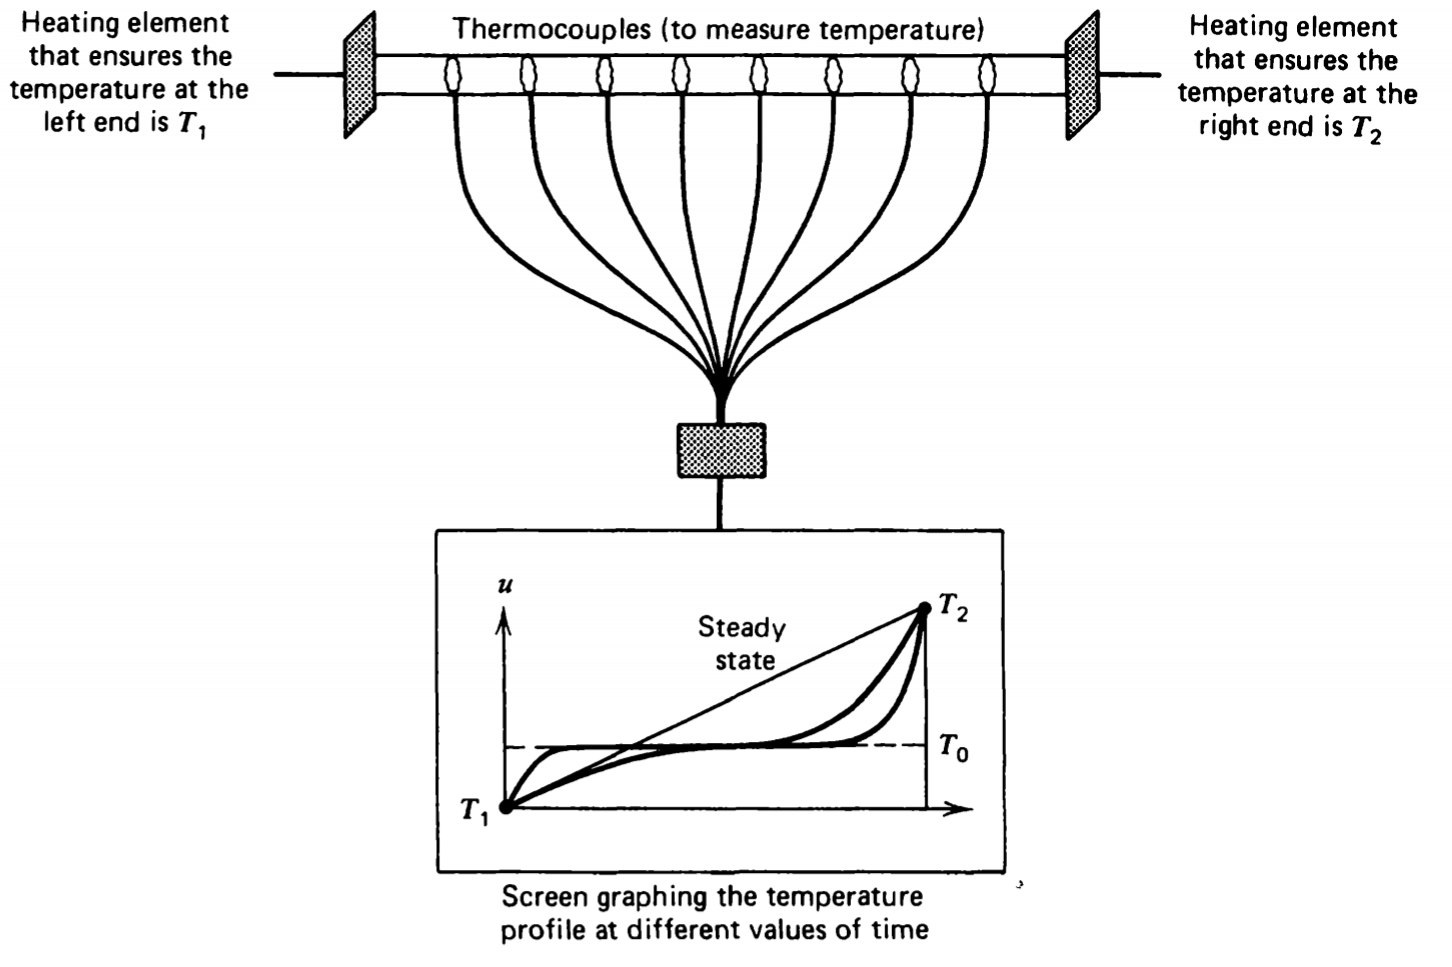
\includegraphics[scale=0.5]{copper.png}
\end{figure}

At time $t=0$, the temperature in the rod is known.
\begin{align*}
u(0,x) = T_0
\end{align*}
The ends of the rod are placed in thermal baths which hold their temperatures fixed. So, at $x=0$, $u(t,0) = T_1$ and at $x=L$, $u(t,L) = T_2$ for all $t>0$.
\subsection{The Mathematical Model}
This behavior is modeled by the heat equation. 
\begin{align*}
u_t = \alpha^2 u_{xx},
\end{align*}
where $\alpha \in \mathbb{R}$, determined by the thermo-character of the rod. $u_t$ is the rate of change of temperature in time, and $u_{xx}$ is the concavity profile in space. \\

Some justification for the heat equation: we look at the spatial difference quotient. For small change in $x$, $\Delta x$:
\begin{align*}
u_{xx} &\approx \frac{u_x(t,x+\Delta x) - u_x(t,x)}{\Delta x}\\
&\approx \frac{(u(t,x+\Delta x) - u(t,x))/\Delta x - (u(t,x)-u(t,x-\Delta x))/\Delta x}{\Delta x}\\
&\approx \frac{1}{\Delta x^2}(u(t,x+\Delta x) + u(t,x-\Delta x) - 2u(t,x))\\
&\approx \frac{2}{\Delta x^2}\left(\frac{u(t,x+\Delta x) + u(t,x-\Delta x)}{2} - u(t,x) \right)
\end{align*}
So, $u_{xx} \propto$ the difference between the average temperatures among neighboring points and the temperature at $x$. 
\begin{figure}[h!]
	\centering
	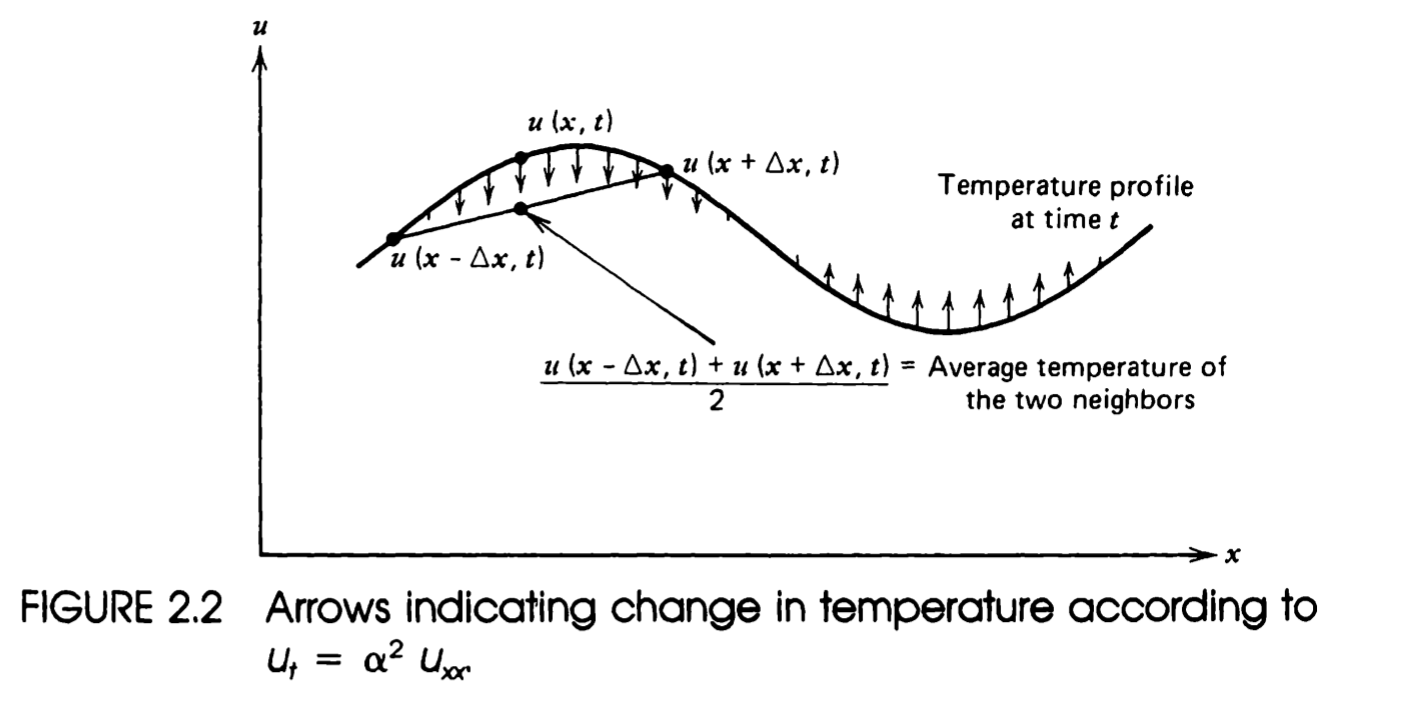
\includegraphics[scale=0.5]{copper1.png}
\end{figure}

Assume that $u_t = \alpha^2 u_{xx}$, then if $u_{xx} < 0$, then $u_t < 0$, i.e. temperature decreases in time. If $u_{xx} > 0$, then $u_t > 0$, i.e. temperature increases in time. If $u_{xx} = 0$, the temperature stays fixed. 

% Feb 11, 2019
\subsection{Boundary Conditions}
In contrast to ODEs, PDE have different types of constraints which are combined with the PDE to form well-posed problems, where ``well-posed'' means that a unique solution exists. Our conditions are often (and will almost always) be physically motivated. \\

Let us revisit the heat equation. 
\begin{align*}
u_t = \alpha^2 u_{xx}, t> 0, 0\leq x\leq L.
\end{align*}
The temperatures at the ends $x=0$ and $x=L$ are fixed $T_1$ and $T_2$ by the thermal baths, so the boundary conditions are
\begin{align*}
BCs = \begin{cases*}
u(0,t) = T_1\\
u(L,t) = T_2
\end{cases*}
\forall t > 0.
\end{align*} 
Here ``boundary'' refers to the boundary of $[0,L]$.
\subsection{Initial Conditions}
Our problem also involves evolution in time, we have an initial condition of the form
\begin{align*}
u(x,0) = T_0 \text{ or } u(x,0) = u_0(x) \forall x \in [0,L]
\end{align*}
where $T_0$ is the initial constant temperature of the rod and $u_0(x)$ is the initial temperature which is allowed to vary (some spatial distribution). All together, we form an initial boundary value problem, an IBVP of the form
\begin{align*}
\begin{cases*}
u_t = \alpha^2 u_{xx}, t>0,x\in[0,L]\\
u(0,t) = T_1, \forall t > 0\\
u(L,t) = T_2,\forall t > 0\\
u(x,0) = T_0, \forall x\in[0,L]
\end{cases*} 
\end{align*}
\subsection{A Couple of Variants}
\subsubsection{Lateral Heat Loss}
This allows for heat to be transferred laterally into the rod according to Newton's law of cooling. So the new heat equation is
\begin{align*}
u_t = \alpha^2 u_{xx} -\beta(u - u_0), \beta > 0
\end{align*}
where $u_0$ is the outside temperature.
\subsubsection{Internal Heat Source}
If, by some non-diffusive heat source, heat is added into the rod at $(t,x)$, the equation is
\begin{align*}
u_t = \alpha^2 u_{xx} + f(x,t)
\end{align*}
where $f(x,t)$ is the heat added to the rod, internally. This PDE is \textit{inhomogeneous}.
\subsubsection{Diffusion-convection Equation}
\begin{align*}
u_t = \alpha^2 u_{xx} - vu_x
\end{align*}
If $u$ describes the amount (not heat) pollutant, then the term $-vu_x$ describes the flow of additional pollutant introduced by the moving particles. 
\subsubsection{Variable-coefficients case}
When the thermal make up of the rod (its thermal character) is allowed to vary according to a variable diffusivity coefficient, i.e. $\alpha \rightarrow \alpha(x)$, then the relevant heat equation is
\begin{align*}
u_t = \alpha^2(x)u_{xx}.
\end{align*}
So, let's say
\begin{align*}
\alpha(x) = 
\begin{cases*}
\alpha_{Copper}, x\in[0,L/2]\\
\alpha_{Bronze}, x\in[L/2,L]
\end{cases*}
\end{align*}
\newpage
\section{Other types of Boundary Conditions}
\subsection{Type 1}
Let's revisit the original heat equation: $u_t = \alpha^2 u_{xx}$. If we force the rod ends to have time-dependent temperatures: $g_1(t)$ and $g_2(t)$ at $x=0$ and $x=L$ respectively, then our boundary conditions are
\begin{align*}
BCs = 
\begin{cases*}
u(0,t) = g_1(t)\\
u(L,t) = g_2(t)
\end{cases*}
\forall t > 0.
\end{align*} 
If instead we're studying the heat flow on a circular plate, i.e., where $u = u(t,t,\theta)$, and the heat EQ is 
\begin{align*}
u_t = \alpha^2 \nabla^2 u = \alpha^2\left( u_{rr} + \frac{1}{r}u_r + \frac{1}{r^2}u_{\theta\theta} \right).
\end{align*}
Here, the boundary conditions look like $u(t,r_0,\theta) = g(t,\theta)$, i.e. we force the disk to have temperature $g(t,\theta)$ along the boundary.
\subsection{Type 2 (more realistic)}
We take into account heat transfer to rod ends via thermal bath. Suppose that our rod is placed in bath (liquid) at each end of temperature $g_1(t)$ and $g_2(t)$ respectively. 
\begin{figure}[h!]
	\centering
	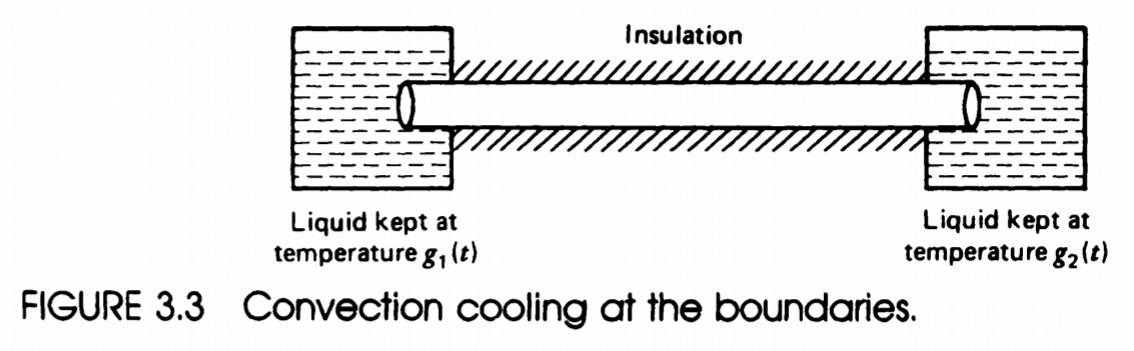
\includegraphics[scale=0.7]{type2.png}
\end{figure}

In view of Newton's law of cooling, the heat flux at a rod end is $h(u(t,0) - g_(1))$ at $x=0$ and $h(u(t,L)-g_2(t))$ at $x=L$, and $h$ is some constant. Next, we introduce Fourier's law of heat flux (empirical):
\begin{align*}
\frac{\p u}{\p n} = k \times\text{Heat flux}
\end{align*}
where $n$ is the \textit{inward normal} direction to the boundary, and $k\in\R$. At $x=0$:
\begin{align*}
\begin{cases*}
\frac{\p u}{\p n} = u_x(t,0) = kh(u(t,0)-g_1(t)), x=0\\
\frac{\p u}{\p n} = -u_x(t,L) = kh(u(t,L)-g_2(t)), x=L
\end{cases*}.
\end{align*}
So, the BC for Type 2 is the following
\begin{align*}
\begin{cases*}
u_x(t,0) = kh(u(t,0) - g_1(t))\\
u_2(t,L) = -kh(u(t,L) - g_2(t))
\end{cases*}
\end{align*}
The 2-D plate analogue is the following. We require (since $r$ is outward)
\begin{align*}
-\frac{\p u}{\p r} = -kh(u(t,r_0,\theta) - g(t,\theta))
\end{align*}
where $g(t,\theta)$ is the temperature of the bath surrounding the plate. 


\subsection{Type 3: Flux specified - including isolated boundaries} 
The rod ends are insulated, i.e., no heat flows in or out of the rod ends. So the boundary conditions are
\begin{align*}
u_x(0,t) = u_x(L,t) = 0 \forall 0 < t < \infty.
\end{align*}
In two variables (a disk), the analogous BC is
\begin{align*}
u_r(t,r_0,\theta) = 0 \forall 0 < t < \infty, 0\leq \theta \leq 2\pi.
\end{align*}
\subsection{Type 4: Mixed}
We can mix BCs. Suppose that one end of the rod has zero flux condition (type 3) and the other end is submerged in a liquid (type 2).

\begin{figure}[h!]
	\centering
	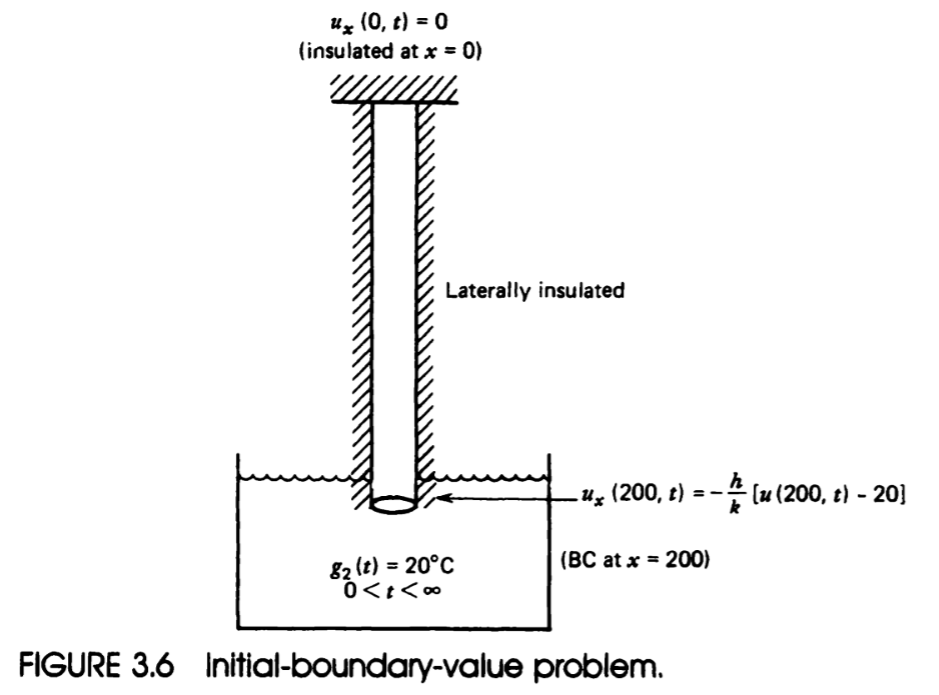
\includegraphics[scale=0.7]{type4.png}
\end{figure}

So, the IBVP is
\begin{align*}
\begin{cases*}
u_t = \alpha^2 u_xx\\
u_x(t,L) = 0\\
u_x(t,0) = -\lambda(u(t) - g_1(t)) \forall t > 0\\
u(0,x) = u_0(x) \forall 0\leq x \leq L
\end{cases*}
\end{align*}
\newpage
\section{Derivation of the Heat Equation}
\begin{figure}[h!]
	\centering
	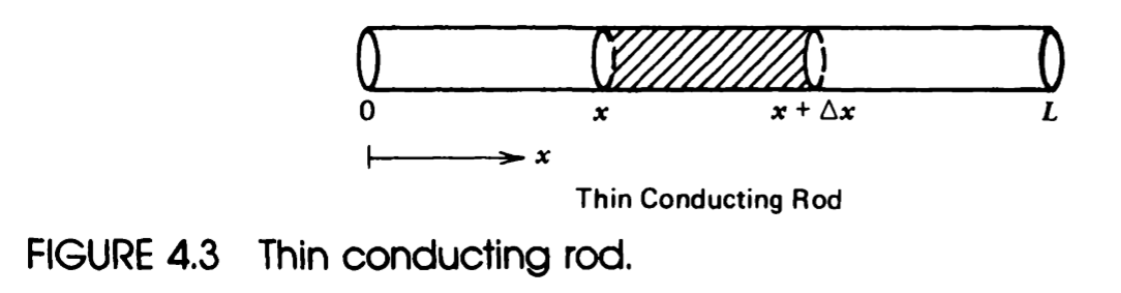
\includegraphics[scale=0.3]{heat.png}
\end{figure}
Main idea: Conservation of (Heat) Energy. Assumptions:
\begin{enumerate}
	\item The rod is a thermally homogeneous material 
	\item The temperature is constant across all cross-sections
	\item The rod is laterally insulated (no heat loss laterally)
\end{enumerate}
Using conservation of energy, we have the following: the change in thermal energy in the cross section $x$ to $x+\Delta x$ should be equal to the flux of the heat through the ``ends'' at $x$ and $x+\Delta x$ plus any external heat produced by some source (e.g. heat element). Some physical constants:
\begin{enumerate}
	\item $C$: thermal capacity of the rod
	\item $\rho$: density of the material of the rod
	\item $A$: area of cross section
	\item $k$: thermal conductivity
\end{enumerate}
Total heat inside is
\begin{align*}
\int_{x}^{\Delta x + x}c\rho A u(s,t)\,ds.
\end{align*}
The flux through the ends is
\begin{align*}
kA(u_x(x+\Delta x,t) - u_x(x, t)).
\end{align*}
The external energy is
\begin{align*}
A\int_x^{x+\Delta x}f(t,s)\,ds
\end{align*}
where $f(t,s)$ is the energy added at time $t$ and $x\leq s \leq x+\Delta x$. All together
\begin{align*}
\frac{d}{dt}\int_{x}^{\Delta x + x}c\rho A u(s,t)\,ds = kA(u_x(x+\Delta x,t) - u_x(x, t)) + A\int_x^{x+\Delta x}f(t,s)\,ds.
\end{align*}
Assuming that $u$ is nice enough, that
\begin{align*}
\frac{d}{dt}\int_{x}^{\Delta x + x}c\rho A u(s,t)\,ds = \int_{x}^{\Delta x + x}c\rho A u_t(s,t)\,ds.
\end{align*}
Also, the MVT for integrals says that if $G$ is continuous on the interval $[a,b]$ then $\exists c\in[a,b]$ such that
\begin{align*}
\int_a^b G(s)\,ds = G(c)(b-a).
\end{align*}
Therefore $\exists \chi \in [x,\Delta x]$ such that
\begin{align*}
\int_{x}^{\Delta x + x}c\rho A u_t(s,t)\,ds = c\rho A u_t(t,\chi)\Delta x
\end{align*}
and $\exists \eta \in [x,\Delta x]$ such that
\begin{align*}
A\int_x^{x+\Delta x}f(t,s)\,ds = Af(t,\eta)\Delta x.
\end{align*}
Combining all of these gives $\forall t > 0, \exists \chi,\eta \in [x,\Delta x]$ such that
\begin{align*}
c\rho Au_t(t,\chi)\Delta x &= kA(u_x(t,x+\Delta x) - u_x(t,x)) + Af(t,\eta)\Delta x\\
u_t(t,\chi) &= \frac{k}{\rho c}\frac{u_x(t,x+\Delta x) - u_x(t,x)}{\Delta x} + \frac{1}{c\rho}f(t,\eta).
\end{align*}
As $\Delta x \rightarrow 0$, $\eta,\chi \rightarrow x$
\begin{align*}
u_t(t,x) &= \frac{k}{\rho c}u_{xx}(x,t) + \frac{1}{c\rho}f(t,x)\\
u_t(t,x) &= \frac{k}{\rho c}u_{xx}(x,t) + F(t,x)\\
u_t(t,x) &= \alpha^2 u_{xx}(x,t) + F(t,x),
\end{align*}
where
\begin{align*}
\alpha^2 &= \frac{k}{\rho c}\\
F(t,x) &= \frac{1}{c\rho}f(t,x).
\end{align*}
\newpage
\section{Separation of Variables - First method of solution}
Main idea: If the IBVP is posed on a rectangle, e.g. $t>0,x\in[0,L]$, and the PDE is linear, it is often the case that this method reduces the PDE into ODEs. 
\subsection{Example: The heat equation}
\begin{align*}
u_t = \alpha^2 u_{xx}, t>0, x\in[0,1]
\end{align*}
We shall accompany this with so-called linear homogeneous BCs:
\begin{align*}
\alpha u(t,0) + \beta u_x(t,0) = 0\\
\gamma u(t,1) + \delta u_x(t,1) = 0.
\end{align*}
In fact, we specify further to assume
\begin{align*}
u(t,0)=0=u(t,1)\forall t > 0.
\end{align*}
We make an ansatz that solutions are of the form
\begin{align*}
u(t,x) = T(t)X(x).
\end{align*}
(Maybe not solutions but builidng blocks of solutions). Plug into the PDE, we get
\begin{align*}
u_t(t,x) = T'(t)X(x) = \alpha^2\p_x^2(u(t,x)) = \alpha^2 T(t)X''(x). 
\end{align*}
Separating variables gives
\begin{align*}
\frac{T'(t)}{\alpha^2 T(t)} = \frac{X''(x)}{X(x)} \forall t>0, x\in[0,1].
\end{align*} 
For this equation to hold for all independent $t$ and $x$, we must have that 
\begin{align*}
\frac{T'(t)}{\alpha^2 T(t)} = \frac{X''(x)}{X(x)} = \text{Const} \forall t>0, x\in[0,1].
\end{align*}
This immediately gives two ODEs connected by a constant $k$:
\begin{align*}
\begin{cases}
T(t) = \alpha^2 k T(t)\\
X''(x) = kX(x)
\end{cases}.
\end{align*}
By solving these equations, we hope to learn something aboaut $k$. The solution to the first solution is obvious:
\begin{align*}
K(t) = Ae^{\alpha^2 kt} \forall t > 0. 
\end{align*}
For physically reasonable solutions, we expect that the limit as $t\to \infty$ of $u(t,x) = 0$ and so, $T(t)\not\to\infty$ as $t\to\infty$, this forces $k<0$. Thus, we write $k=-\lambda^2$, $\lambda\in\R$, and denote
\begin{align*}
u_\lambda(t,x) = T(t)X(x) = X(x)Ae^{-\alpha^2\lambda^2t}.
\end{align*}
Next, the spatial ODE gives
\begin{align*}
X''(x) + \lambda^2 X(x) = 0.
\end{align*}
A general solution for this equation is
\begin{align*}
X(x) = A\sin(\lambda x) + B\cos(\lambda x).
\end{align*}
By absorbing multiplcative constants
\begin{align*}
u_\lambda(t,x) = e^{-\alpha^2\lambda^2 t}\left(A\sin(\lambda x) + B\cos(\lambda x) \right).
\end{align*}
Though we still don't know what $\lambda$ is, let us force this solution to satisfy the boundary conditions to learn more. Since the boundary conditions require that $u(t,0)=0=u(t,1)$, we require that
\begin{align*}
\begin{cases}
B=0\\
\lambda = \pm n\pi
\end{cases}
\end{align*}
where $n\in \mathbb{N}$, for non-trivial solutions (where $A\neq 0$). Thus, with separation of variables, we find that
\begin{align*}
u_n(t,x) = A_ne^{-(n\alpha\pi)^2}\sin(n\pi x).
\end{align*}
This is a solution for any $n\in \mathbb{N}$ and $A_n\in\R$. Just to be sure that we haven't made an error, we can readily verify this solution. This is left as an exercise to the reader. \\

Note that we still have some ``degrees of freedom'' - $A_n$ and $n$. So, we have established the existence of \textit{many} solutions, for each $n\in\mathbb{N}$ and $A_n\in\R$. Now, we make use of the principle of superposition to generate more solutions. The principle of superposition (works for linear DEs) says that all convergent sums of solutions are solutions. More generally, for any collection $\{A_n \} \subseteq\R$,
\begin{align*}
u(t,x) = \sum_{n=1}^\infty A_n e^{-(n\pi\alpha)^2}\sin(n\pi x)
\end{align*}
is also a solution. But divergence could be a problem here. It might be that $u(t,x)$ fails to exist, or differentiation might not work. But worry not, since the presence of the term $e^{-(n\pi\alpha)^2}$ makes this series always converge. And so, we have that for any sequence $\{ A_n\}$, $u(t,x)$ defined in this way solves the DE $u_t = \alpha^2 u_{xx}$ and satisfies the boundary conditions $u(t,0)=0=u(t,1)$. The problem of satisfying the initial condition $u(0,x) = u_0$ becomes one of finding the ``right'' constants $A_n$ so that 
\begin{align*}
u(0,x) = \sum_{n=1}^\infty A_n\sin(n\pi x) = u_0(x).
\end{align*} 

% feb 18, 2019} 
The term on the left hand side is called the trigonometric series. The question now becomes whether it is possible to find the sequence $\{ A_n\} \subseteq \R$ so that
\begin{align*}
u(0,x) = \sum_{n=1}^\infty A_n \sin (n \pi x) = u_0(x).
\end{align*}
Another question would be which function $u_0(x)$ can be expanded as a trigonometric series as above.

\begin{exmp}
	Consider
	\begin{align*}
	u_0(x) = \frac{1}{2}\sin(2\pi x) + \frac{1}{50}\sin(201\pi x).
	\end{align*}
	We see that
	\begin{align*}
	A_n = 0, A_2 = \frac{1}{2}, A_{201} = \frac{1}{50} \forall n\neq 2,201.
	\end{align*}
\end{exmp}

\begin{exmp}
	What about
	\begin{align*}
	u_0(x) = \begin{cases}
	x, 0\leq x < \frac{1}{2}\\
	1-x, \frac{1}{2} < x \leq 1
	\end{cases}
	\end{align*}
	or
	\begin{align*}
	u_0(x) = 1?
	\end{align*}
\end{exmp}


It's clear that we must have that $u_0(0) = u_1(1) = 0$, otherwise this cannot be done. To treat otherwise, one needs a cosine term. But what if $u_0(0) = u_0(1) = 0$, but $u_0(x)$ is very bad? Suppose that this can be done. Using the property that 
\begin{align*}
\int_{0}^1 \sin(n\pi x)\sin(m\pi x) = \frac{1}{2}\delta^m_n,
\end{align*}
we use \textbf{Fourier's trick}: multiply both sides of the $u_0(x)$ expansion by $\sin(m \pi x)$ and integrate:
\begin{align*}
\int^1_0 u_0(x)\sin(m \pi x) &= \sum_{n=1}^\infty\int_{0}^1A_n\sin(n\pi x)\sin(m \pi x)\,dx\\
&= \sum_{n=1}^\infty A_m\frac{1}{2}\delta^m_n.
\end{align*}
So this gives
\begin{align*}
A_m = 2\int^1_0 u_0(x)\sin(m\pi x)\,dx \forall m\in \mathbb{N}.
\end{align*}
This gives a prescription for finding the sequence $\{A_m \}$ so that the expansion works. So, we might ask, given a function $u_0(x)$ with value 0 at $x=0,1$ and define
\begin{align*}
A_m = 2\int^1_0 u_0(x)\sin(m\pi x)\,dx\,\,\, \forall m\in \mathbb{N},
\end{align*}
when does 
\begin{align*}
u_0(x) = \sum^\infty_{n=1}A_n \sin(n\pi x)?
\end{align*}
Usually, this works perfectly, but around 1802, the mathematician DuBois Reymond found an example for which the \textbf{Fourier series} does not hold. The exact class of such functions was determined explicitly in 1962 by UCLA professor L. Carelson. The answer is $L^2[0,1]$ - square integrable functions. \\

\begin{exmp}
	Now, let's find $A_n$ so that 
	\begin{align*}
	u_0(x) = \begin{cases}
	x, 0\leq x < \frac{1}{2}\\
	1-x, \frac{1}{2} < x \leq 1
	\end{cases}.
	\end{align*}
	Well,
	\begin{align*}
	A_n &= 2\int_{0}^1 u_0(x)\sin(n\pi x)\,dx = 2\int_{0}^\frac{1}{2} x\sin(n\pi x)\,dx + 2\int_{\frac{1}{2}}^1 (1-x)\sin(n\pi x)\,dx\\
	&= 2\int_{0}^\frac{1}{2} x\sin(n\pi x)\,dx - 2\int_\frac{1}{2}^1 +  x\sin(n\pi x)\,dx + 2\int_{\frac{1}{2}}^1 \sin(n\pi x)\,dx
	\end{align*}
	Integration by parts...
	\begin{align*}
	\int x\sin(kx)\,dx = \frac{-1}{k}x\cos(kx) - \int \frac{-\cos(kx)}{k}\,dx = \frac{1}{k^2}\sin(kx) - \frac{x\cos(kx)}{k}.
	\end{align*}
	So
	\begin{align*}
	2\left( \frac{1}{(n\pi)^2}\sin(n\pi x) - \frac{x}{\pi n}\cos(n\pi x)
	 \right)\bigg\vert^{1/2}_0
	 = \frac{2}{(n\pi)^2}\sin\left( \frac{n\pi}{2}\right)  - \frac{1}{n\pi}\cos\left( \frac{n\pi}{2}\right).
	\end{align*}
	\begin{align*}
	2\int_{\frac{1}{2}}^1 (1-x)\sin(n\pi x)\,dx = 
	\frac{2}{n\pi}\left( \cos\left(\frac{n\pi}{2} \right)  - \cos(n\pi)\right).
	\end{align*}
	\begin{align*}
	2\int_\frac{1}{2}^1 x\sin(n\pi x)\,dx = \frac{2}{n\pi}\cos(n\pi) - \frac{2}{(n\pi)^2}\sin\left( \frac{n\pi}{2} \right) + \frac{1}{n\pi}\cos\left(\frac{n\pi}{2} \right).
	\end{align*}
	So, all together,
	\begin{align*}
	A_n = \frac{4}{(n\pi)^2}\sin\left( \frac{n\pi}{2}\right).
	\end{align*}
	So our series is
	\begin{align*}
	u_0(x) = \sum_{n=1}^\infty \frac{4}{(n\pi)^2}\sin\left( \frac{n\pi}{2}\right) \sin(n\pi x)
	\end{align*}
	This converges nicely. 
\end{exmp}

Recap: to solve our IVBP, we defines 
\begin{align*}
A_n = 2\int_{0}^1 u_0(x)\sin(n\pi x)\,dx, \,\,\, n\in \mathbb{N}
\end{align*}
and then (provided that things converge nicely)
\begin{align*}
u(t,x) = \sum_{n=1}^\infty A_n e^{-(\alpha \pi n)^2 t}\sin(n\pi x)
\end{align*}
is \textbf{the} solution. More generally, on the interval $[0,L]$ for the same IVBP with $u(t,0) = u(t,L) = 0$ and $u(0,x) = u_0(x), x\in[0,L]$, then the solution is given by
\begin{align*}
u(t,x) = \sum_{n=1}^\infty A_n e^{-(\alpha \pi n/L)^2 t}\sin\left(\frac{n\pi x}{L}\right)
\end{align*}
where 
\begin{align*}
A_n = \frac{2}{L}\int_{0}^1 u_0(x)\sin\left(\frac{n\pi x}{L}\right)\,dx, \,\,\, n\in \mathbb{N}.
\end{align*}
One more note: as $t\to \infty$, the solution is dominated lower order terms
\begin{align*}
u(t,x)\approx A_1 e^{-(\alpha \pi/L)^2 t}\sin\left(\frac{\pi x}{L}\right).
\end{align*}





\newpage
\section{Transforming Nonhomogeneous Boundary Conditions into Homogeneous ones }

\subsection{Inhomogeneous BCs to Homogeneous Ones}

Question: how can we solve inhomogeneous BCS? Given $k_1,k_2\in\R$ and $u_0(x)$, can we solve
\begin{align*}
\begin{cases}
u_t = \alpha^2u_{xx}\\
u(t,0) = k_1\\
u(t,L) = k_2\\
u(0,x) = u_0(x)
\end{cases}
\end{align*}

Idea: in the steady-state, we expecet that $u_t = 0$, so $u(x,t) \to u(x) = Cx+D$. So, the steady state is
\begin{align*}
S(t,x) = k_1\left( 1 - \frac{x}{L} \right) + k_2\left(\frac{x}{L} \right).
\end{align*}
To solve the problem, we assume 
\begin{align*}
u(t,x) = S(t,x) + U(t,x)
\end{align*}
where $S(t,x)$ is the steady-state solution, and $U(t,x)$ is the transient solution. Let's plug $u = S+U$ into our problem to learn something about $U$. First, 

\begin{align*}
u_t = S_t + U_t &= \alpha^2 (S_{xx} + U_{xx})\\
U_t &= \alpha^2 U_{xx}.
\end{align*}
Using the BCs in out IBVP,
\begin{align*}
k_1 = u(t,0) = S(t,0) + U(t,0) = k_1 + U(t,0).
\end{align*}
So
\begin{align*}
U(t,0) = 0.
\end{align*}
And similarly,
\begin{align*}
U(t,L) = 0.
\end{align*}
Finally, 
\begin{align*}
u_0(x) = u(0,x) = S(0,x) + U(0,x)
\end{align*}
and hence
\begin{align*}
U(0,x) = u_0(x) - S(0,x).
\end{align*}
So, summary: $u(t,x)$ satisfies the IBVP $\iff$ 
\begin{align*}
u(t,x)=S(t,x)+U(t,x) = k_1\left( 1 - \frac{x}{L} \right) + k_2\left(\frac{x}{L} \right) + U(t,x)
\end{align*}
where $U(t,x)$ solves the auxiliary IBVP:


\begin{align*}
\begin{cases}
U_t = \alpha^2U_{xx}\,\,\,\, t>0,0<x<L\\
U(t,0) = 0\,\,\, t> 0\\
U(t,L) = 0\\
U(0,x) = u_0(x) - S(0,x)\,\,\,\,\, x\in[0,L]
\end{cases},
\end{align*}
which we know how to solve using separation of variables and Fourier series. 

\subsection{Time Varying BCs into Zero BCs}
\begin{align*}
\begin{cases}
u_t = \alpha^2u_{xx}\,\,\,\,, t>0,0<x<L\\
\alpha_1 u(t,0) + \beta_1 u_x(t,0) = g_1(t)\\
\alpha_2 u(t,L) + \beta_2 u_x(t,L) = g_2(t)\\
u(0,x) = u_0(x)\,\,\,\,\,, x\in[0,L]
\end{cases},
\end{align*}
where $\alpha_1,\alpha_2,\beta_1,\beta_2,g_1(t),g_2(t),u_0(x)$ are all known. To solve this, we push forwardour idea of steady-state-ish and transient solutions. We assume that 
\begin{align*}
u(t,x)= S(t,x) + U(t,x)
\end{align*}
where
\begin{align*}
S(t,x) = A(t)\left( 1 - \frac{x}{L}\right) + B(t)\frac{x}{L}
\end{align*}
Can we find $A(t)$ and $B(t)$ in terms of $\alpha_1,\alpha_2,\beta_1,\beta_2,g_1(t),g_2(t),u_0(x)$? We want to choose $S(t,x)$ so that it absorbs all of the \textit{complicated} nature of the BCs for $u(t,x)$. So, we can make $S$ satisfy $u's$ BCs. 
\begin{align*}
S(t,0)&= A(t)\\
S_x(t,0) &= \frac{B(t) - A(t)}{L}  = S_x(t,L)\\
S(t,L) &= B(t).
\end{align*}
So we have
\begin{align*}
\alpha_1 S(t,0) + \beta_1 S_x(t,0) &= g_1(t)\\
\alpha_1 A(t) + \frac{\beta_1(B(t) - A(t))}{L} &= g_1(t)
\end{align*}
and
\begin{align*}
\alpha_2 S(t,L) = \beta_2 S_x(t,L) &= g_2(t)\\
\alpha_2 B(t) + \frac{\beta_2(B(t) - A(t))}{L} &= g_2(t).
\end{align*}
Rewriting gives
\begin{align*}
\Gamma\begin{pmatrix}
A(t)\\B(t)
\end{pmatrix} = 
\begin{pmatrix}
\alpha_1 - \frac{\beta_1}{L} & \frac{\beta_1}{L}\\
- \frac{\beta_2}{L} & \alpha_2  + \frac{\beta_2}{L}
\end{pmatrix}
\begin{pmatrix}
A(t)\\B(t)
\end{pmatrix}
=
\begin{pmatrix}
g_1(t)\\g_2(t)
\end{pmatrix}
\end{align*}
So
\begin{align*}
\begin{pmatrix}
A(t)\\B(t)
\end{pmatrix} = \Gamma^{-1}\begin{pmatrix}
g_1(t)\\g_2(t)
\end{pmatrix}=
\begin{pmatrix}
\rho_{11}(t)&\rho_{12}(t)\\
\rho_{21}(t) & \rho_{22}(t)
\end{pmatrix}
\begin{pmatrix}
g_1(t)\\g_2(t)
\end{pmatrix}
\end{align*}
Of course, this requires $\Gamma$ to be invertible, i.e, 
\begin{align*}
\det(\Gamma) = \left(\alpha_1 - \frac{\beta_1}{L}\right)\left(\alpha_2  + \frac{\beta_2}{L}\right) +  \frac{\beta_1}{L}\frac{\beta_2}{L} = \alpha_1 \alpha_2 + \frac{\alpha_1\beta_2}{L} - \frac{\alpha_2\beta_1}{L}\neq 0.
\end{align*}
Assuming this is true
\begin{align*}
S(t,x) = (\rho_{11}g_1(t) + \rho_{12}g_2(t))\left(1 - \frac{x}{L} \right) + (\rho_{21}g_1(t) + \rho_{22}g_2(t))\frac{x}{L}
\end{align*}
Now, let us see what this implies for $U$. 
\begin{align*}
u_t = S_t + U_t = U_t = \alpha^2(S_{xx} +  U_{xx}) = \alpha^2 U_{xx}.
\end{align*}
So, once again
\begin{align*}
U_t = \alpha^2 U_{xx} - S_t.
\end{align*}
Also, by an easy calculation, we have that $u$ satisfying the inhomogeneous BCs implies
\begin{align*}
U(t,0) = U(t,L) = 0.
\end{align*}
And further, that
\begin{align*}
U(0,x)= u_0 - S(0,x)
\end{align*}
is just a linear function of $x$. So, by setting 
\begin{align*}
S(t,x)= (\rho_{11}g_1(t) + \rho_{12}g_2(t))\left(1 - \frac{x}{L} \right) + (\rho_{21}g_1(t) + \rho_{22}g_2(t))\frac{x}{L},
\end{align*}
we see that
\begin{align*}
u(t,x) = U(t,x) + S(t,x)
\end{align*}
satisfies a IBVP where the heat equation is homogeneous, but the BCs are very complicated compared to the new inhomogeneous heat IBVP. 
\begin{align*}
\begin{cases}
U_t = \alpha^2 U_{xx} - S_t\\
U_x(L,t) = 0\\
U(t,L) = 0\\
U(0,x) = u_0(x) - S(0,x)
\end{cases}.
\end{align*}
Moral: problems with complicated BCs can often be transformed into equivalent problems with simple BCs at the cost of making the PDE more complicated. \\

Question: Under what conditions on the first IBVP is our new IBVP homogeneous? The answer is that a sufficient condition is for $g_1$, $g_2$ to be constant. In this realm, $S(t,x) = S(x)$ nad is thus a ``real'' steady-state solution.

\newpage

\section{Solving more complicated problems directly: An invitation to Strum-Liouville theory}

Consider the following IBVP:
\begin{align*}
\begin{cases}
u_t = \alpha^2 u_{xx}\\
u(t,0) = 0\\
u_x(t,1) + hu(t,1) = 0\\
u(0,x) = u_0(x) 
\end{cases}.
\end{align*}
We can solve this using separation of variables. First, we seek product solutions of the form:
\begin{align*}
u(t,x) = T(t)X(x).
\end{align*}
By asking that $u_t = \alpha^2 u_{xx}$, we obtained 
\begin{align*}
\frac{T'(t)}{\alpha^2 T(t)} = \frac{X''(x)}{X(x)} = \mu
\end{align*}
where $\mu$ is a constant. What are the possibilities for $\mu$?\\

\subsection{$\mu > 0$}
If $\mu>0$, we obtain
\begin{align*}
u(t,x) = Ae^{\alpha^2 \mu t}X(x).
\end{align*}
But as $e^{\alpha^2 \mu t} \to \infty$ as $t\to\infty$, we reject this solution on physical grounds. \\
\subsection{$\mu=0$}
If $\mu = 0$, then $T'(t) = X''(x) = 0$, so
\begin{align*}
u(t,x) = Ax+b.
\end{align*}

To satisfy the BCs in this case:
\begin{align*}
u(t,0) = 0 = A\times 0 + b.
\end{align*}
So, $b=0$. Next,
\begin{align*}
u_x(t,1) + hu(t,1) = 0.
\end{align*}
So, $A+hA = 0$, so $A=0$. This is just the trivial solution.

\subsection{$\mu <0$}
Let $\mu=\lambda^2$, then we have
\begin{align*}
T(t) = Ae^{-(\alpha \lambda)^2t}
\end{align*}
and
\begin{align*}
X(x) = A\sin(\lambda x) + B\cos(\lambda x).
\end{align*}
So,
\begin{align*}
u(t,x) = e^{-(\lambda\alpha)^2t}\left( A\sin(\lambda x) + B\cos(\lambda x) \right).
\end{align*}
We let this subject to BCs:
\begin{align*}
u(t,0) = e^{-(\lambda\alpha)^2t}\left( A\sin(\lambda\times 0) + B\cos(\lambda \times 0) \right) = 0.
\end{align*}
So, $B=0$. Thus our product solution looks like
\begin{align*}
u(t,x) = Ae^{-(\lambda\alpha)^2t}\sin(\lambda x).
\end{align*}
The other BC gives
\begin{align*}
0=u(t,1)+hu_x(t,1)=Ae^{-(\lambda\alpha)^2t}\left( \lambda\cos(\lambda) + h\sin(\lambda) \right).
\end{align*}
So,
\begin{align*}
\tan\lambda - \frac{-\lambda}{h}.
\end{align*}

So, admissible $\lambda$'s here are solution to this equation, which is not as simple as $\pi n$, like we have found before. Now, note that $\lambda$ is this equation cannot be found explicitly. Solutions are just intersections on the following plot:
\begin{figure}[h!]
	\centering
	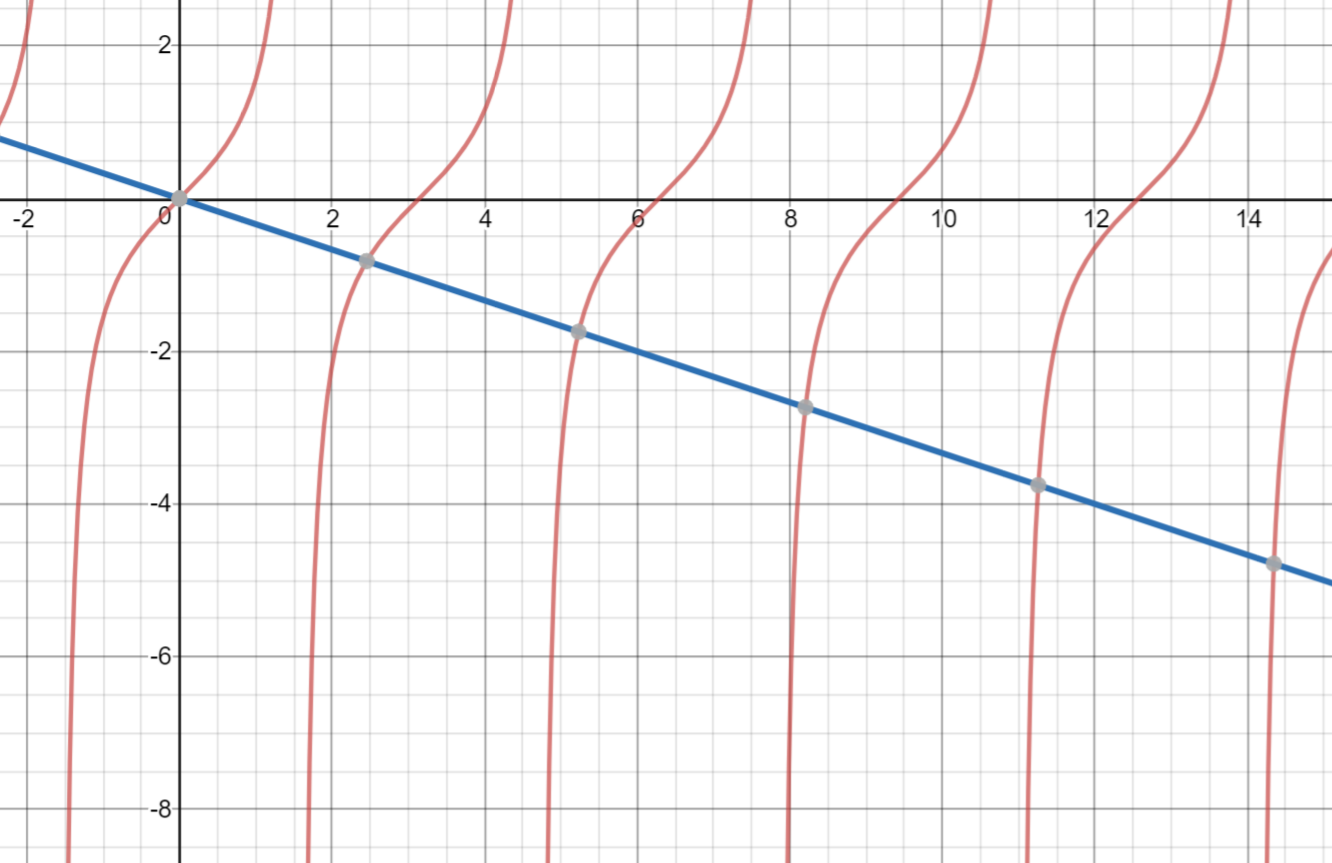
\includegraphics[scale=0.6]{tan.png}
\end{figure}

We see that
\begin{align*}
\frac{\pi}{2} < \lambda_1 < \pi < \lambda_2 < 2pi < \lambda_3 < 3\pi.
\end{align*}
We call these $\lambda_n$'s eigenvalues associated with the boundary value problem
\begin{align}
\begin{cases}
X'' + \lambda^2 X = 0\\
X(0) = 0\\
X'(1) + hX(1) = 0
\end{cases}.
\end{align}
The solutions, $\sin(\lambda_n x)$ are associated eigenfunction. So, with separation of variables, we obtain
\begin{align*}
u_n(x,t) = A_n e^{-(\lambda_n\alpha)^2t}\sin(\lambda_n x)
\end{align*}
which solve the IBVP. Once again, we have that
\begin{align*}
u(t,x) = \sum_{n=1}^{\infty} A_n e^{-(\lambda_n\alpha)^2t}\sin(\lambda_n x)
\end{align*}
which we want to also satisfy the IC, which is 
\begin{align*}
u(0,x) = u_0(x).
\end{align*}
We invoke Fourier's trick to find $A_n's$:
\begin{align*}
\int_{0}^1 u_0(x)\sin(\lambda_m x)\,dx &= \int_{0}^1 \sin(\lambda_m x)\sum_{n=1}^{\infty} A_n e^{-(\lambda_n\alpha)^2t}\sin(\lambda_n x)\,dx\\
&= \sum_{n=1}^\infty A_n\int_{0}^1 \sin(\lambda_m x)\sin(\lambda_n x)\,dx\\
&= A_m \left( \frac{1}{2} - \frac{\sin(2\lambda_m x)}{4\lambda_m} \right).
\end{align*}
So
\begin{align*}
\int_{0}^1 u_0(x)\sin(\lambda_m x) \,dx &= A_m \frac{1}{2\lambda_m}\left( \lambda_m - \sin(\lambda_m x)\cos(\lambda_m x) \right)
\end{align*}
and so
\begin{align*}
A_m = \frac{2\lambda_m}{\lambda_m - \sin(\lambda_m x)\cos(\lambda_m x)}\int_{0}^1 u_0(x)\sin(\lambda_m x) \,dx.
\end{align*}

\noindent Summary: Recall the IBVP:
\begin{align*}
\begin{cases}
u_t = \alpha^2 u_{xx}\\
u(t,0) = 0\\
u_x(t,1) + hu(t,1) = 0\\
u(0,x) = u_0(x) 
\end{cases}.
\end{align*}
In trying to solve it, we have found
\begin{align*}
u(t,x) \sum_{n=1}^{\infty}A_n e^{-(\alpha \lambda)^2t}\sin(\lambda_n x)
\end{align*}
to be a solution with
\begin{align*}
A_m = \frac{2\lambda_m}{\lambda_m - \sin(\lambda_m x)\cos(\lambda_m x)}\int_{0}^1 u_0(x)\sin(\lambda_m x) \,dx.
\end{align*}
where $\lambda_n$ is the n$^{th}$ positive solution to 
\begin{align*}
\frac{-\lambda}{n}= \tan(\lambda)
\end{align*}
Question: In our finding of $A_n$, we swept a detail under the rug. It was \textbf{orthogonality}. We assumed the fact that for all $n,m$
\begin{align*}
\int^1_0 \sin(\lambda_m x)\sin(\lambda_n x)\,dx = 0,\,\,\,\,\,\,\text{ if } m\neq n.
\end{align*}
This would be obvious if $\lambda_n = n\pi$. But it is not the case here. We will look at this in the next section.
\newpage
\section{ODE Boundary Value Problems - a look at the Sturm-Liouville theory}
(reference: Boyce-DiPrima, Chapter 11).\\


Motivating example:
\begin{align*}
\begin{cases}
ODE: y'' + \lambda y = 0\\
BC: y(0) = y(1) = 0, 0\leq x\leq 1.
\end{cases}.
\end{align*}
We ask: does solving this BVP require anything about $\lambda$? Is it possible to find non-zero solutions to this problem for arbitrary $\lambda$? We can try...\\

If $\lambda = 0$, then $y(x) = Ax+B$. By subjecting to the BCs, we get $A=B=0$. So, not every $\lambda$ gives a non-trivial solution. This $\lambda$ does not admit non-zero solutions. This is in stark contrast to IVP which can be solved for any non-zero $\lambda$.\\

If $\lambda < 0$, we get the same issue (can check that there are no non-zero solutions for $\lambda< 0$. \\

If $\lambda > 0$, then $y(x) = C_1 \sin(\sqrt{\lambda} x ) + C_2 \cos(\sqrt{\lambda} x)$. Subject to boundary conditions, we have $C_2 = 0$ and
\begin{align*}
C_1 = \sin(\sqrt{\lambda} x).
\end{align*}
For non-trivial solutions,
\begin{align*}
\sqrt{\lambda}=n\pi.
\end{align*}
Or for $n=1,2,3,\dots$
\begin{align*}
\lambda_n = n^2 \pi^2.
\end{align*}

The moral: Not every $\lambda$ works. So we ask: Given a linear ODE and linear homogeneous BCs, which $\lambda$ (if any) will work?\\

\begin{defn}
	\textbf{General theory:} Consider the ODE
	\begin{align*}
	(p(x)y')' - q(x)y + \lambda r(x)y = 0,
	\end{align*}
	where we will let $p,q,r \in C^0([0,1])$. Moreover, $p(x) \in C^1([0,1])$. Finally, $p(x),r(x) > 0$ for all $x\in[0,1]$. Also, consider the linear homogeneous BCs:
	\begin{align*}
	a_1y(0) + b_1y'(0) &= 0\\
	a_2y(1) + b_2y'(1) &= 0.
	\end{align*}
	
	If, for some fixed $\lambda$, the ODE and the BCs have a non-zero solution $\phi(x)$, we say that $\lambda$ is an \textbf{eigenvalue} for the BVP, and $\phi(x)$ is an \textbf{eigenfunction} corresponding to $\lambda$. \\
	
	An eigenvalue $\lambda$ corresponding to the BVP is said to be simple if it does not have two linearly independent eigenfunctions $\phi_1, \phi_2$. 
	\qed
\end{defn}

\begin{rmk}
	$\,$\\
	\begin{enumerate}
		\item We will write 
		\begin{align*}
		L[y] = -(p(x)y')' + q(x)y,
		\end{align*}
		which is a second-order linear operator. Then the ODE becomes:
		\begin{align*}
		L[y] = \lambda r(x)y.
		\end{align*}
		For this reason, we see the ``eigen'' terminology arises. 
	\end{enumerate}
\end{rmk}

Given our ODE, the theory of ODE gives, for fixed $\lambda$, two linearly independent solutions of the form $y_1 = y_1(x,\lambda), y_2 = y_2(x,\lambda)$, and so all solutions to the ODE is of the form
\begin{align*}
y(x) = C_1 y_1(x,\lambda) + C_2y_2(x,\lambda).
\end{align*}
Question: can we find a condition on $\lambda$ so that $y$ above is a non-zero solution satisfying the BCs? Sure we can. Let us subject $y$ to the BCs. We have
\begin{align*}
0 = a_1y(0) + b_1 y'(0) =& a_1(C_1y_1(0,\lambda) + C_2y_2(0,\lambda)) + b_1(C_1y'_1(0,\lambda) + C_2y'_2(0,\lambda))\\
&= C_1(a_1y_1(0,\lambda) + b_1y'_1(0,\lambda)) + C_2(a_1y_2(0,\lambda) + b_1y'_2(0,\lambda)).
\end{align*}
Similarly, 
\begin{align*}
0 = C_1(a_2y_1(1,\lambda) + b_2y'_1(1,\lambda)) + C_2(a_2y_2(1,\lambda) + b_2y'_2(1,\lambda)).
\end{align*}
As a matrix equation,
\begin{align*}
A\begin{pmatrix}
C_1\\C_2
\end{pmatrix}=
\begin{pmatrix}
0\\0
\end{pmatrix}=
\begin{pmatrix}
a_1y_1(0,\lambda) + b_1y'_1(0,\lambda) & a_1y_2(0,\lambda) + b_1 y'_2(0,\lambda)\\
a_2y_1(1,\lambda) + b_2y'_1(1,\lambda) & a_2y_2(1,\lambda) + b_2y'_2(1,\lambda)
\end{pmatrix}
\begin{pmatrix}
C_1\\C_2
\end{pmatrix}.
\end{align*}
To get non-trivial solution, we require that $\ker(A)\neq \{ 0\}$, i.e., $\det(A) = 0$. This gives a necessary and sufficient condition on $\lambda$, since $a_i,b_i$ and the solutions are known, that is
\begin{align*}
\boxed{\det(A)=0}
\end{align*}

% Feb 27, 2019 % 

Recall that $$ L[y] = -(p(x)y')' + q(x)y.$$ So the ODE is $$ L[y] = \lambda r(x) y.$$ 

\begin{prop}
	\textbf{Lagrange's Identity:} For any $u,v \in \mathbb{C}^2([0,1])$, the following identity holds:
	\begin{align*}
	\int^1_0 (uL[v] - vL[u])\,dx = p(x)\left( u'(x)v(x) - u(x)v'(x) \right)\bigg\vert^1_0.
	\end{align*}
	Intuitively, this is essentially an integration by parts formula for the operator $L$.
	
	
	\begin{proof}
		We have
		\begin{align*}
		u(x)L[v](x) - v(x)L[u](x) &= u(x)(-(p(x)v')' + q(x)v) - v(x)(-(p(x)u')' + q(x)u)\\
		&= -u(x)(p(x)v'(x))' + u(x)q(x)v(x)\\ &\hspace{0.5cm}+ v(x)(p(x)u(x))' - q(x)v(x)u(x)\\
		&= -u(x)(p(x)v'(x))' + v(x)(p(x)u(x))'.
		\end{align*}
		So the integral becomes
		\begin{align*}
		\int^1_0 (uL[v] - vL[u])\,dx &= \int^1_0 -u(x)(p(x)v'(x))' + v(x)(p(x)u(x))'\,dx\\
		&= \int^1_0 -u(x)(p(x)v'(x))' \,dx    + \int^1_0 v(x)(p(x)u(x))' \,dx\\
		&= -u(x)(p(x)v'(x))\bigg\vert^1_0 - \int^1_0 -u'(x)p(x)v'(x)\,dx\\ &\hspace{0.5cm}+v(x)(p(x)u'(x))\bigg\vert^1_0 - \int^1_0 v'(x)(p(x)u'(x))\,dx\\
		&= p(x)\left(v(x)u'(x) - u(x)v'(x)\right)\bigg\vert^1_0.
		\end{align*}
	\end{proof}
\end{prop}

\textbf{Corollary:} If $u,v$ are eigenfunctions for the BVP then
\begin{align*}
\int_0^1 (uL[v] - vL[u])\,dx = 0.
\end{align*}
\begin{proof}
	Recall the boundary conditions: 
	\begin{align*}
	a_1u(0) + b_1u'(0) &= 0\\
	a_1v(0) + b_1v'(0) &= 0\\
	a_2u(1) + b_2u'(1) &= 0\\
	a_2v(1) + b_2v'(1) &= 0
	\end{align*}
	Assume that $b_1,b_2\neq 0$. For $\phi = v$ or $u$,
	\begin{align*}
	\phi'(0) &= \frac{-a_1}{b_1}\phi(0)\\
	\phi'(0) &= \frac{-a_2}{b_2}\phi(1).
	\end{align*}
	So
	\begin{align*}
	\int_0^1 (uL[v] - vL[u])\,dx &= p(x)\left(v(x)u'(x) - u(x)v'(x)\right)\bigg\vert^1_0\\
	&= p(1)\left(v(1)u'(1) - u(1)v'(1)\right) - p(0)\left(v(0)u'(0) - u(0)v'(0)\right)\\
	&=\dots\\
	&= 0.
	\end{align*}
\end{proof}


	\textbf{Theorem: All eigenvalues associated with the Sturm-Liouville problem are real.}  
\begin{proof}
	Let $\lambda = u + iv$ and $\phi =U + iV$ are an eigenvalue-eigenfunction pair associated with the BVP. Then
	\begin{align*}
	L[\phi] = \lambda r(x)\phi.
	\end{align*}
	Conjugating and noting that $p,q,r$ are real give	
	\begin{align*}
	L[\phi]^* &= (\lambda r(x)\phi)^*\\
	&= ((-p(x)\phi'(x))' + q(x)\phi(x))^*\\
	&= (-p(x)\phi^{*'})' + q(x)\phi^*\\
	&= L[\phi^*].
	\end{align*}
	This gives
	\begin{align*}
	L[\phi^*] = \lambda^* r(x)\phi^*.
	\end{align*}
	This says that $\lambda^*$ is an eigenvalue too, which takes $\phi^*$ as an eigenfunction. So, $(\lambda^*,\phi^*)$ and $(\lambda,\phi)$ are two eigenvalue-eigenfunction pairs. By the corollary:
	\begin{align*}
	0 &= \int_{0}^1 (\phi L[\phi^*] - \phi^* L[\phi])\,dx\\
	&= \int^1_0 (\lambda^* -\lambda)r(x)\vert \phi(x)\vert^2\,dx
	\end{align*}
	Since $r(x) > 0$ for all $x$, and $\phi$ is non-zero, 
	\begin{align*}
	\vert \phi(x)\vert^2 > 0
	\end{align*}
	for some non-trivial interval in $[0,1]$. So
	\begin{align*}
	(\lambda^* -\lambda)\int^1_0 r(x)\vert \phi(x)\vert^2\,dx > 0.
	\end{align*}
	And so 
	\begin{align*}
	\lambda^* = \lambda,
	\end{align*}
	i.e., $\lambda \in \mathbb{R}$.
\end{proof}



	\textbf{Theorem: ORTHOGONALITY - Sweeping under the carpet:} Let $\lambda_1$ and $\lambda_2$ be distinct eigenvalues with eigenfunctions $\phi_1$ and $\phi_2$. Then 
	\begin{align*}
	\int^1_0 r(x)\phi_1(x)\phi_2(x)\,dx = 0.
	\end{align*} 
	\begin{proof}
		We have, by the corollary, that
		\begin{align*}
		0 &= \int^1_0 (\phi_1L[\phi_2] - \phi_2L[\phi_1])\,dx\\
		&= \int_{0}^1 r(x)\phi_1\lambda_2\phi_2 - \phi_2\lambda_1r(x)\phi_1\,dx\\
		&= (\lambda_2 - \lambda_1)\int^1_0 r(x)\phi_1\phi_2\,dx.
		\end{align*}
		Since the eigenvalues are distinct, the integral must be zero.
	\end{proof}
%Mar 1, 2019%
So, if $\phi_1$ and $\phi_2$ were eigenfunctions corresponding to distinct eigenvalues $\lambda_1, \lambda_2$ then $\phi_1$ and $\phi_2$ are orthogonal in the sense given by the theorem. \\

But how do we know $\phi$'s exist?\\

\textbf{Theorem:} Given a Sturm-Liouville problem, there exist eigenvalues and eigenfunctions. The collection of eigenvalues forms an infinite sequence $\{\lambda_n\}$ for which $\lambda_1<\lambda_2 <\dots$ and $\lambda_n\to \infty$ as $n\to\infty$, Further, each eigenvalue is simple. (Note: this has to do with the spectral theorem).\\

The final result is another important theorem. But first we define a few things. 
\begin{defn}
	An eigenfunction for the Sturm-Liouville problem is said to be normalized if 
	\begin{align*}
	\int^1_0 \phi^2 r(x)\,dx = 1.
	\end{align*}
\end{defn}

\begin{defn}
	In view of the Sturm-Liouville problem, a function $f$ is admissible with respect to the S-L problem if it is continuous, piecewise differentiable on $[0,1]$ and 
	\begin{enumerate}
		\item If $b_1 = 0$ then $f(0) = 0$.
		\item If $b_2 = 0$ then $f(1) = 0$.
	\end{enumerate}
\end{defn}

\textbf{Theorem: Completeness.} Let $\{ \phi_n\}$ be the sequence of normalized eigenfunctions to the S-L problem. 
\begin{enumerate}
	\item If $f$ is admissible with respect to the S-L problem, then $f(x)$ can be expressed as
	\begin{align*}
	\sum_{i=1}^\infty a_i \phi_i(x)\,dx
	\end{align*}
	where
	\begin{align*}
	a_i = \int^1_0 f(x)\phi_i(x)r(x)\,dx.
	\end{align*}
	and $f(x)$ converges pointwise. 
\end{enumerate}


\begin{exmp}
	Consider a S-L problem:
	\begin{align*}
	&u'' + \lambda u = 0\\
	&\begin{cases}
	u(0)=0\,\,\,\, (a_1=1,b_1=0)\\
	u(1) = 0\,\,\, (a_2=1, b_2=0)
	\end{cases}
	\end{align*}
	We found that
	\begin{align*}
	\lambda_n = (n\pi)^2
	\end{align*}
	with the eigenfunctions being $\{\sqrt{2} \sin(n\pi x) \}$. The theorem says if $f$ is a continuous, piecewise differentiable functions on the interval $[0,1]$vwith $f(0) = 0 = f(1)$, then 
	\begin{align*}
	f(x) = \sum^\infty_{n=1}a_n\left(\sqrt{2}\sin(n\pi x)\right)\,\,\,\, (\text{Fourier series})
	\end{align*}
	where 
	\begin{align*}
	a_n = \int^1_0 f(x)\left(\sqrt{2}\sin(n\pi x) \right)\,dx
	\end{align*}
\end{exmp}

Observe that for the S-L problem we have the linear operator $L : u \to L[u]$:
\begin{align*}
L[u] = -(p(x)u')' + q(x)u.
\end{align*}
$L$ is a linear operator initially defined on $C^2([0,1])$ (twice-differentiable functions on) and $L : C^2([0,1])\to C^0([0,1])$. So, given boundary conditions for the problem of the form 
\begin{align*}
&a_1u(0) + b_1u'(0) = 0\\
&a_2u(1) + b_2u'(1) = 0,
\end{align*}
any twice differentiable functions $u,v$ which satisfy the boundary conditions have the following property that 
\begin{align*}
\int^1_0 uL[v] - vL[u]\,dx = 0.
\end{align*}
If, say
\begin{align*}
\langle f,g \rangle = \int^1_0 f(x)g(x)\,dx
\end{align*}
then 
\begin{align*}
\langle u,L[v]\rangle = \langle L[u],v\rangle.
\end{align*}
Such an operator $L$ is said to be (formally) self-adjoint. 

















%Mar 4 2019%
\newpage
\section{Transforming Hard Equations into Easier Ones}
In this section we will learn how to solve the IBVP of a laterally-heat-losing rod.
\begin{align*}
&u_t = \alpha^2 u_{xx} - \beta u\\
&\begin{cases}
u(t,0) = 0 = u(t,1)\\u(0,x) = u_0(x)
\end{cases}
\end{align*}
Ansatz: we will assume (so that the $\beta$ term goes away)
\begin{align*}
u(t,x) = e^{-\beta t}w(t,x).
\end{align*}
Can we convert an equation for $u$ into an easier equation for $w$. Plug in, we get:
\begin{align*}
- \beta e^{\beta t}w(t,x) + e^{-\beta t}w_t(t,x) = \alpha^2 e^{-\beta t}w''(t,x) - \beta e^{-\beta t}w(t,x).
\end{align*}
This gives a nice equation for $w$:
\begin{align*}
w_t = \alpha^2 w_{xx}.
\end{align*}
A moment's thougt shows that all of these steps are reversible. This means that $w$ solves $w_t = \alpha^2 w_{xx} \iff$ $u$ solves $u_t = \alpha^2 u - \beta u$.\\

The boundary and initial conditions are exactly the same. In fact, $u$ satisfies the BCs and ICs $\iff$ $w$ satisfies the same ones:
\begin{align*}
\begin{cases}
w(t,0) = 0 = w(t,1)\\
w(0,x) = u(0,x) = u_0(x).
\end{cases}
\end{align*}
So, we wish to solve the following problem:
\begin{align*}
&w_t = \alpha^2 w_{xx}\\
&\begin{cases}
w(t,0) = 0 = w(t,1)\\w(0,x) = u_0(x)
\end{cases}.
\end{align*}
The solution is of course
\begin{align*}
w(t,x) = \sum^\infty_{i=1}a_n e^{-(n\pi \alpha)^2t}\sin(n\pi x)
\end{align*}
where 
\begin{align*}
a_n = 2\int^1_0 u_0(x)\sin(n\pi x)\,dx.
\end{align*}
So
\begin{align*}
u(t,x) &= e^{-\beta x}w(t,x)\\ &= e^{-\beta t}\sum^\infty_{i=1}a_n e^{-(n\pi \alpha)^2t}\sin(n\pi x)\\
&= \sum^\infty_{i=1}a_n e^{-[(n\pi \alpha)^2 + \beta] t}\sin(n\pi x).
\end{align*}
Since $\beta>0$, $u(t,x)\to 0$ faster than if $\beta = 0$. 

\newpage

\section{Solving Nonhomogeneous PDEs (Eigenfunction Expansion)}
In all we've done, we haven't yet attack an inhomogeneous heat equation. Let's set out to solve the problem 
\begin{align*}
&u_t = \alpha^2 u_{xx} + f(t,x)\\
&\begin{cases}
u(t,0) = 0\\
u(t,1) = 0
\end{cases}
u(0,x) = u_0(x).
\end{align*}
The method we shall follow will also solve the more general problem 
\begin{align*}
&u_t = \alpha^2 u_{xx} + f(t,x)\\
&\begin{cases}
a_1u(t,0) + b_1u_x(t,0) = 0\\
a_2u(t,1) + b_2u_x(t,1) = 0
\end{cases}
u(0,x) = u_0(x).
\end{align*}
The question is: Can we write the solution as a series of products:
\begin{align*}
u(t,x) = \sum^\infty_{n=0}T_n(t)X_n(x)?
\end{align*}
Recall that we've expanded things via Fourier series (generally to deal with $u_0$) or general eigenfunction expansions from the Sturm-Liouville theory. So, can we also expand $f(t,x)$ in this way?\\

%Mar 6. 2019%
Consider the (easy) inhomogeneous problem. 
\begin{align*}
&u_t = \alpha^2 u_{xx} + f(t,x)\\
&\begin{cases}
u(t,0) = 0\\
u(t,1) = 0
\end{cases}
u(0,x) = u_0(x).
\end{align*}
We will solve with via eigenfunction expansion...
\begin{enumerate}
	\item Decompose $f$ into pieces so that
	\begin{align*}
	f(t,x) = \sum^\infty_{n=1}f_n(t)X_n(x)
	\end{align*}
	where $X_n$'s arise by solving the associated homogeneous problem:
	\begin{align*}
	&u_t = \alpha^2 u_{xx}\\
	&\begin{cases}
	u(t,0) = 0\\
	u(t,1) = 0
	\end{cases}
	u(0,x) = u_0(x).
	\end{align*}
	To this end, we write the solution
	\begin{align*}
	u(t,x) = \sum^\infty_{n=1}T_n(t)X_n(x)
	\end{align*}
	where $X_n$'s solve the Strum-Liouville problem:
	\begin{align*}
	&X'' - \alpha^2 X_{xx} = 0\\
	&\begin{cases}
	X(0) = 0\\
	X(1) = 0
	\end{cases}
	\end{align*}
	For this particular problem, 
	\begin{align*}
	X_n(x) = \sin(n\pi x).
	\end{align*}
	With the assumption that the function $X \to f(t,x)$ is admissible in the Sturm-Liouville sense for all $t$, the result from $S-L$ theory gives that 
	\begin{align*}
	f(t,x) = \sum_{n=1}^\infty f_n(t)X_n(x),
	\end{align*}
	where
	\begin{align*}
	f_n(t) = 2\int^1_0 f(t,x)\sin(n\pi x)\,dx.
	\end{align*}
	
	
	
	
	\item Subject
	\begin{align*}
	u(t,x) = \sum^\infty_{n=1}T_n(t)X_n(x)
	\end{align*}
	to the IBVP, where
	\begin{align*}
	f(t,x) = \sum_{n=1}^\infty f_n(t)X_n(x),
	\end{align*}
	and
	\begin{align*}
	X_n(x) = \sin(n\pi x),
	\end{align*}
	we get
	\begin{align*}
	u_t(t,x) = \sum^\infty_{n=1}\dot{T}_n(t)\sin(n\pi x),
	\end{align*}
	and
	\begin{align*}
	u_{xx}(t,x) = \sum^{\infty}_{n=1}-(n\pi)^2T_n(t)\sin(n\pi x).
	\end{align*}
	Into the IBVP, $u_t = \alpha^2 u_{xx}$
	\begin{align*}
	\sum^\infty_{n=1}\dot{T}_n(t)\sin(n\pi x) = \alpha^2 \sum^{\infty}_{n=1}-(n\pi)^2T_n(t)\sin(n\pi x) + \sum_{n=1}^\infty f_n(t)\sin(n\pi x),
	\end{align*}
	or equivalently,
	\begin{align*}
	\sum^\infty_{n=1}\left[\dot{T}_n(t) + (\alpha n\pi)^2T_n(t)\right]\sin(n\pi x) = \sum_{n=1}^\infty f_n(t)\sin(n\pi x).
	\end{align*}
	This yields ODEs of the form:
	\begin{align*}
	\dot{T}_n(t) + (\alpha n\pi)^2T_n(t) = f_n(t),\hspace{0.5cm}n=1,2,3,\dots
	\end{align*}
	to which the solution is of the form
	\begin{align*}
	T_n(t) = e^{-(\alpha n\pi)^2t}\int_0^t f_n(s) e^{(\alpha n \pi)^2s} \,ds + T_n(0)e^{-(\alpha n \pi)^2t}. 
	\end{align*}
	Note, for
	\begin{align*}
	u(0,x) = \int^\infty_{n=1} T_n(0)\sin(n\pi x) = u_0(x),
	\end{align*}
	which means the choice of the Fourier Sine coefficients
	\begin{align*}
	T_n(0) = 2\int^1_0 u_0(x)\sin(n\pi x)\,dx, \hspace{0.5cm}n=1,2,3,\dots
	\end{align*}
	does the trick. Thus, the original IBVP is satisfied $^{(?)}$ with
	\begin{align*}
	u(t,x) = \sum^\infty_{n=1} \left(e^{-(\alpha n\pi)^2t}\int_0^t f_n(s) e^{(\alpha n \pi)^2s} \,ds + T_n(0)e^{-(\alpha n \pi)^2t}\right)\sin(n\pi x),
	\end{align*}
	where
	\begin{align*}
	&T_n(0) = 2\int^1_0 u_0(x)\sin(n\pi x)\,dx, \hspace{0.5cm}n=1,2,3,\dots\\
	&f_n(t) = 2\int^1_0 f(t,x)\sin(n\pi x)\,dx, \hspace{0.5cm}n=1,2,3,\dots
	\end{align*}
	We write this as
	\begin{align*}
	u(t,x) = \sum^\infty_{n=1} \left(e^{-(\alpha n\pi)^2t}\int_0^t f_n(s) e^{(\alpha n \pi)^2s} \,ds \right)\sin(n\pi x) + \sum^\infty_{n=1}T_n(0)e^{-(n\pi \alpha)^2t}\sin(n\pi x),
	\end{align*}
	where the first term is the steady-state solution, and the second term is the transient solution, because in the second term, as $t\to \infty$ it goes to zero. Let's check that this works. 
	\begin{enumerate}
		\item Note that $u(t,0) = u(t,1) = 0.$
		\item And
		\begin{align*}
		u(0,x) = 0 + \sum^\infty_{n=1}T_n(0)e^{-(n\pi \alpha)^2t}\sin(n\pi x) = u_0(x),
		\end{align*}
		which is true by design.
		\item We can also check that it solves the PDE, but we won't...
	\end{enumerate}
	
\end{enumerate}

\begin{exmp}
	\begin{align*}
	\begin{cases}
	u_t = u_{xx} + x - x^2\\
	u(t,0) = u(t,1) = 0\\
	u(0,x) = u_0(x) = \sin(\pi x).
	\end{cases}
	\end{align*}
	\begin{sln*}
		Here, $f(t,x) = x - x^2$. So
		\begin{align*}
		f_n(t) &= 2\int^1_0 (x-x^2)\sin(n\pi x)\,dx\\
		&= 2\left( (x-x^2)\frac{\cos(n\pi x)}{-n\pi}\bigg\vert^1_0 - \int^1_0(1-2x)\frac{\cos(n\pi x)}{-n\pi}\,dx \right)\\
		&= 0 + \frac{2}{n\pi}\int^1_0 (1-2x)\cos(n\pi x)\,dx\\
		&= \frac{2}{n\pi}\left( (1-2x)\frac{\sin(n\pi x)}{n\pi}\bigg\vert^1_0 - \frac{2}{n\pi}\int^1_0(-2)\frac{\sin(n\pi x)}{n\pi}\,dx \right)\\
		&= \frac{4}{(n\pi)^2}\int^1_0 \sin(n\pi x)\,dx\\
		&= \frac{4}{(n\pi)^3}(-\cos(n\pi x))\bigg\vert^1_0\\
		&= \frac{4}{(n\pi)^3}(1-(-1)^n).
		\end{align*}
		Also,
		\begin{align*}
		T_n(0) = \int^1_0u_0(x)\sin(n\pi x)\,dx,
		\end{align*}
		but since $u_0(x) = \sin(\pi x)$,
		\begin{align*}
		T_n(0) = \delta^1_n.
		\end{align*}
		Now,
		\begin{align*}
		\int_0^t f_n(s) e^{( n \pi)^2s} \,ds &= \int_0^t \frac{4}{(n\pi)^3}(1-(-1))^n e^{( n \pi)^2s} \,ds\\
		&= \frac{4}{(n\pi)^5}(1-(-1)^n)\left(e^{(n\pi)^2t} - 1\right).
		\end{align*}
		All together...
		\begin{align*}
		u(t,x) &= \sum^\infty_{n=1} \left(e^{-( n\pi)^2t}\left(\frac{4}{(n\pi)^5}(1-(-1)^n)\left(e^{(n\pi)^2t} - 1\right) \right)\right)\sin(n\pi x) + e^{-(\pi )^2t}\sin(\pi x).
		\end{align*}
	\end{sln*}
\end{exmp}

%Mar 8, 2019%
Physically, what does this solution say? First, we have a diffusion term. But not only that, we have $u_t \sim x-x^2$, i.e., we're adding heat to the middle of the rod and allowing this heat to diffuse. We can also approximate the solution to get
\begin{align*}
u(t,x) &= \sum^\infty_{n=1} \left(e^{-( n\pi)^2t}\left(\frac{4}{(n\pi)^5}(1-(-1)^n)\left(e^{(n\pi)^2t} - 1\right) \right)\right)\sin(n\pi x) + e^{-(\pi )^2t}\sin(\pi x)\\
&\approx \frac{8}{\pi^5}\sin(\pi x) + \left(1 - \frac{8}{\pi^5}\right)e^{-\pi^2 t}\sin(\pi x).
\end{align*}
So this makes sense, because the temperature distribution is $\sin(\pi x)$ scaled down by some number. 



\newpage


\section{Integral Transformation}
An integral transformation/operator is a map taking a function $f$ to another function $F = \I[f]$ by the rule:
\begin{align*}
\boxed{\I[f](s) = \int^B_A \K(s,t)f(t)\,dt}
\end{align*}
where $\K(s,t)$ is called an \textbf{integral kernel}.\\

\begin{prop}
	Integral operators are linear (when taken to be defined on some appropriate vector space of functions). 
	\begin{proof}\textit{-ish}\\
		
		Let $f,g$ be given. Then
		\begin{align*}
		\I[\alpha f+ \beta g](s) &= \int^B_A \K(s,t)\left(\alpha f(t) + \beta g(t)\right)\,dt\\
		&= \alpha \int^B_A \K(s,t)f(t)\,dt + \beta \int^B_A \K(s,t)g(t)\,dt\\
		&= \alpha\I[f](s) + \beta\I[g](s).
		\end{align*}
	\end{proof}
\end{prop}

\textbf{Note}: The study of integral transformations is a main focus of functional analysis. \\

\textbf{Note}: We can think of this as moving between spaces: momentum and position. \\

In many cases, an integral transformation $\I$ will have an inverse, denoted $\I^{-1}$, so that, in particular, if $F(s) = \I[f](s)$ then $f(t) = \I^{-1}[F](t)$, i.e.,
\begin{align*}
\I^{-1}\circ \I = \text{Identity}.
\end{align*}
For us, presently, we will work with integral transformations to take difficult PDEs and transform them into simple PDEs which are easier to solve . Taking the solution to the easier PDE and applying the inverse transformation will yield the solution to the harder PDE.\\

Idea: Hard PDE $\to$ Easier PDE $\to$ Solution to easy PDE $\to$ Solution to hard PDE.\\

\textbf{Note}: there's some resemblance between this and ``change of basis.''\\

\subsection{Some common transformations}


\subsubsection{The Fourier Transform}

Works with $f:\R \to \mathbb{C}$.


\begin{align*}
\F[t](\xi) = \hat{f}(\xi) = \frac{1}{\sqrt{2\pi}}\int^\infty_{-\infty} e^{-ix\xi}f(x)\,dx = F(\xi).
\end{align*}
The inverse looks almost exactly the same:
\begin{align*}
\F^{-1}[F](x) = \frac{1}{\sqrt{2\pi}}\int^\infty_{-\infty} e^{ix\xi}F(\xi)\,d\xi = f(x).
\end{align*}
This yields (in the vector space $L^2(\R)$)
\begin{align*}
\F^{-1}\circ \F = \text{Identity}.
\end{align*}

\textbf{Disadvantage}: complex-valued things\\

\textbf{Advantage}: almost always works, and takes differentiation to polynomial multiplication.\\

\textbf{Note}: $\F$ is a unitary operator.

\subsubsection{The Fourier Sine Transform}

\begin{align*}
\F_s[f](w) = \frac{2}{\pi}\int^\infty_{0}\sin(wt)f(t)\,dt.
\end{align*}
The inverse is
\begin{align*}
\F^{-1}_s[F](t) = \int_{0}^\infty\sin(wt)F(w)\,dw.
\end{align*}

\subsubsection{The Fourier Cosine Transform}

\begin{align*}
\F_c[f](w) = \frac{2}{\pi}\int^\infty_{0}\cos(wt)f(t)\,dt.
\end{align*}
The inverse is
\begin{align*}
\F^{-1}_c[F](t) = \int_{0}^\infty\cos(wt)F(w)\,dw.
\end{align*}

\subsubsection{The Discrete/Finite Fourier Transform (Fourier Series)}

Given a function $f : [0,L] \to \R$ or $\mathbb{C}$, the finite Fourier transform

\begin{align*}
\F[f](n) = \hat{f}(n) = a_n = \frac{1}{L}\int^L_0 f(x)e^{-2\pi inx/L}\,dx.
\end{align*}
The inverse is
\begin{align*}
\F^{-1}(n) = \F^{-1}[\hat{f}(n)] = \sum^\infty_{n=-\infty} a_n e^{2\pi inx/L}. 
\end{align*}

\textbf{Property:}
\begin{align*}
f(x) = \sum^\infty_{n=-\infty} \hat{f}(n)e^{inx} = \F^{-1}\circ \F[f].
\end{align*} 

\subsubsection{The Analogous Sine Transform}


\begin{align*}
\F_s[f](n) = a_n = \frac{2}{L}\int^L_0 f(x)\sin\left(\frac{\pi nx}{L}\right)\,dx.
\end{align*}
The inverse is
\begin{align*}
\F^{-1}_s[a_n](x) = \sum^\infty_{n=1}a_n \sin\left(\frac{n\pi x}{L}\right).
\end{align*}

\textbf{Disadvantage:} Half-range expansions...

\subsubsection{The Laplace Transform}

\textbf{Note:} the Laplace transform is analogous to the Moment Generating Function in Probability theory. 

\begin{align*}
\lag[f](s) = \int^\infty_0 e^{-st}f(t)\,dt.
\end{align*}
The (difficult) inverse is
\begin{align*}
\lag^{-1}[F](t) = \frac{1}{2\pi i} \int^{C+i\infty}_{C-i\infty}F(s)e^{st}\,ds,
\end{align*}
which is a complex contour integral.\\



% Mar 11, 2019 %

\subsection{The Fourier Series}
We had:
\begin{align*}
\F_s[f](\omega) = \frac{2}{\pi}\int^1_0 f(x)\sin(\omega x)\,dx\\
\F_c[f](\omega) = \frac{2}{\pi}\int^1_0 f(x)\cos(\omega x)\,dx\\
\F[f](\xi) = \frac{1}{\sqrt{2\pi}}\int^\infty_{-\infty}f(x)e^{-ix\xi}\,dx.
\end{align*}

\begin{prop} Some identities:
	\begin{enumerate}
		\item $\F_s[f'] = -\omega \F_c[f]$\\
		\item $\F_s[f''] = \frac{2}{\pi}\omega f(0) - \omega^2 \F_s[f]$\\
		\item $\F_c[f'] = \frac{-2}{\pi}f(0) + \omega\F_s[f]$\\
		\item $\F_c[f''] = \frac{-2}{\pi}f'(0) - \omega^2 \F_c[f]$.\\
		\item $\F[f'](\xi) = i\xi \F[f] $\\
		\item $F[f''](\xi) = -\xi^2\F[f](\xi)$
	\end{enumerate}
\end{prop}


\begin{rmk}
	In our alternative notation, this says
	\begin{align*}
	\hat{f'}(\xi) = i\xi \hat{f}(\xi).
	\end{align*}
	We notice that the $\hat{\,}$ map converts differentiation to polynomial multiplication.\\
\end{rmk}


\begin{proof}[Proof of propositions 5,6]
	\begin{enumerate}
		\item Proof of 5.: The supposition that $f,f'$ have existent Fourier Transforms, i.e.,
	\begin{align*}
	\int^\infty_{-\infty}f(x)e^{-ix\xi}\,dx, \int^\infty_{-\infty}f'(x)e^{-ix\xi}\,dx
	\end{align*}
	exist for all $\xi$, requires in particular, that
	\begin{align*}
	\lim_{t\to\pm\infty} f(x) = \lim_{t\to\pm\infty} f'(x) = 0.
	\end{align*}
	So, interpreting these as improper Riemann integrals:
	\begin{align*}
	\F[f'](\xi) &= \frac{1}{\sqrt{2\pi}}\int^\infty_{-\infty}f'(x)e^{-ix\xi}\,dx\\
	&= \frac{1}{\sqrt{2\pi}}\lim_{t\to\infty}\int^t_{-t}f'(x)e^{-ix\xi}\,dx\\
	&= \frac{1}{\sqrt{2\pi}}\lim_{t\to\infty}\left( f(x)e^{-ix\xi}\bigg\vert_{-t}^t - \int^t_{-t}f(x)(-i\xi)e^{-ix\xi}\,dx  \right)\\
	&= \frac{1}{\sqrt{2\pi}}\lim_{t\to\infty}\left( f(t)e^{0it\xi} - f(-t)e^{it\xi} -i\xi\int^t_{-t}f(x)e^{-ix\xi}\,dx \right)\\
	&= i\xi \F[f](\xi).
	\end{align*}
	
	\item Proof of 6.: 
	\begin{align*}
	\F[f'](\xi) &= i\xi\F[f'](s)\\
	&= (i\xi)^2\F[f](\xi)\\
	&= -\xi^2 \F[f](\xi).
	\end{align*}
	
	\end{enumerate}
\end{proof}


There's a \textbf{full version} of the Fourier transform that we won't discuss here.\\


Rather, let us use the $\F_s$ transform to solve half-infinite rod heat equation:
\begin{align*}
\begin{cases}
u_t = \alpha^2 u_{xx}, \hspace{0.5cm}0 < x < \infty, t> 0\\
u(t,0) = A, \hspace{0.5cm} t> 0\\
u(0,x) = 0, \hspace{0.5cm} x\geq 0.
\end{cases}
\end{align*}
We start with $u_t = \alpha^2 u_{xx}$. Let's compute the Fourier Sine transform in the variable $x$ (this is sometimes called the \textbf{Partial Fourier Transform}):
\begin{align*}
\F[u_t(t,x)](\omega) &= \frac{2}{\pi}\int^\infty_0 u_t(t,x)\sin(\omega x)\,dx\\
&= \frac{2}{\pi}\frac{\p}{\p t}\left(\int^\infty_0 u(t,x)\sin(\omega x)\,dx  \right)\\
&= \frac{\p}{\p t}\F_s[u(t,x)](\omega).
\end{align*}
We shall call
\begin{align*}
U(t,\omega) = \F_s[u(t,x)](\omega).
\end{align*}
So,
\begin{align*}
\F_s[u_t(t,x)](\omega) = \frac{\p U}{\p t}.
\end{align*}
On the other hand,
\begin{align*}
\F_s[u_{xx}](\omega) &= \frac{2}{\pi}\int^\infty_0 u_{xx}\sin(\omega x)\,dx\\
&= \frac{2}{\pi}\omega u(t,0) - \omega^2 \F_s[u(t,x)](\omega).
\end{align*}
But $u(t,0) = A$ by the boundary condition, so
\begin{align*}
\F_s[u_{xx}](\omega) &= \frac{2A}{\pi}\omega - U(t,\omega).
\end{align*}
Subject to $u_t = \alpha^2 u_{xx}$, we claim:
\begin{align*}
\frac{\p U}{\p t} = \alpha^2\left( \frac{2A\omega}{\pi} - \omega^2U(t,\omega) \right),
\end{align*}
or equivalently,
\begin{align*}
\frac{\p U}{\p t} + \alpha^2\omega^2 U = \frac{2A\omega^2\alpha^2}{\pi}, 
\end{align*}
which is nothing but a linear ODE. Now, can we get an initial condition for this ODE? Yes! Since $u(0,x) = 0$ for all $x$,
\begin{align*}
U(0, \omega) = \F_s[u(0,x)](\omega) = \F_s[0](\omega) = 0.
\end{align*}
Thus, we have transformed an initial condition for our PDE in $u$ into an initial condition in $U$. We get an IVP:
\begin{align*}
\begin{cases}
\frac{\p U}{\p t} + \alpha^2\omega^2 U = \frac{2A\omega^2\alpha^2}{\pi}\\
U(0,\omega) = 0,
\end{cases}
\end{align*}
whose solution is
\begin{align*}
U(t,\omega) = e^{-\omega^2\alpha^2t}\int^t_0\frac{2A}{\pi}\omega^2\alpha^2e^{\omega^2\alpha^2s}\,ds.
\end{align*}
So,
\begin{align*}
U(t,\omega) = \frac{2A}{\pi}\left(1 - e^{-\omega^2\alpha^2 t}\right).
\end{align*}
So, then
\begin{align*}
u(t,x) = \F_s^{-1}[U(t,\omega)] &= \F_s^{-1}\left[ \frac{2A}{\pi}\left(1 - e^{-\omega^2\alpha^2 t}\right) \right](x)\\
&= A\times \text{erfc}\left(\frac{x}{2\alpha\sqrt{t}}\right),
\end{align*}
where 
\begin{align*}
\text{erfc}(y) = \frac{2}{\sqrt{\pi}}\int^\infty_y e^{-t^2}\,dt.
\end{align*}


% Mar 13, 2019%



\subsection{From the Fourier Series to the Fourier Transform}
First, let us find the connection between cosine-sine version of Fourier Series and $\sum () e^{inx}$. Here is a fact: if $f$ is a periodic of period $2L$ and ``nice,'' then
\begin{align*}
f(x) = \frac{a_0}{2} + \sum^\infty_{n=1}a_n\cos\left(\frac{n\pi x}{L}\right) + \sum^\infty_{n=1}b_n\sin\left(\frac{n\pi x}{L}\right) 
\end{align*}
where
\begin{align*}
a_n = \frac{1}{L}\int^L_{-L}f(x)\cos\left(\frac{n\pi x}{L}\right)\,dx
\end{align*}
and
\begin{align*}
b_n = \frac{1}{L}\int^L_{-L}f(x)\sin\left(\frac{n\pi x}{L}\right)\,dx
\end{align*}
for $n=0,1,2,\dots$. We note that ``nice'' is just piecewise differentiable, or weaker, $f \in L^2([0,L])$. \\

We want to connect this with the complex representation of Fourier Series:
\begin{align*}
f(x) = \sum_{n\in \mathbb{Z}} C_n e^{inx\pi/L},
\end{align*}
where 
\begin{align*}
C_n = \frac{1}{2L}\int^L_{-L}f(x)e^{-in\pi x/L}\,dx.
\end{align*}
Recall the Euler's identity:
\begin{align*}
&e^{i\theta} = \cos\theta + i\sin\theta\\
&e^{-\theta} = \cos\theta - i\sin\theta.
\end{align*}
So,
\begin{align*}
C_n &= \frac{1}{2L}\int^L_{-L}f(x)\cos\frac{n\pi x}{L}\,dx - i\frac{1}{2L}\int^L_{-L}f(x)\sin\frac{n\pi x}{L}\,dx\\
&= \frac{a_n - ib_n}{2},\hspace{0.5cm}n=0,1,2,3,\dots
\end{align*}
For $n=-m$, $m=0,1,2,3,\dots$ then
\begin{align*}
C_{-m} = C_n &= \frac{1}{2L}\int^L_{-L}f(x)e^{im\pi x/L}\,dx\\
&= \frac{1}{2L}\int^L_{-L}f(x)\cos\frac{m\pi x}{L}\,dx + i\frac{1}{2L}\int^L_{-L}f(x)\sin\frac{m\pi x}{L}\,dx\\
&= \frac{a_m + ib_m}{2}.
\end{align*}
In other words, for all $n=0,1,2,\dots$
\begin{align*}
&2C_n = a_n - ib_n\\
&2C_{-n} = a_n + ib_n,
\end{align*}
then
\begin{align*}
a_n = C_n + C_{-n}
\end{align*}
and
\begin{align*}
b_n = \frac{C_{-n} - C_n}{i} = i(C_n - C_{-n}).
\end{align*}
Plugging these coefficients into the Fourier Series, we get
\begin{align*}
f(x) &= C_0 + \sum^\infty_{n=1}(C_n + C_{-n})\cos\frac{n\pi x}{L} + \sum^\infty_{n=0}i(C_n - C_{-n})\sin\frac{n\pi x}{L}\\
&= C_0 + \sum^\infty_{n=1}C_n\left(\cos\frac{n\pi x}{L} + i\sin\frac{n\pi x}{L}\right) + \sum^\infty_{n=1}C_{-n}\left(\cos\frac{n\pi x}{L} - i\sin\frac{n\pi x}{L}\right)\\
&= C_0 + \sum^\infty_{n=1}C_ne^{in\pi x/L} + C_{-n}e^{-in\pi x/L}\\
&= \sum_{n\in \mathbb{Z}}C_ne^{in\pi x/L},
\end{align*}
which is exactly the complex representation of the Fourier Series. \\


So, given a $2L$-periodic nice function $f$, we can write
\begin{align*}
f(x) &= \sum_{n\in \mathbb{Z}}C_ne^{in\pi x/L}\\
&= \sum_{n\in \mathbb{Z}}\left(\frac{1}{2L}\int^L_{-L}f(x')e^{-in\pi x'/L}\,dx'\right)e^{in\pi x/L}\\
&= \sum_{n\in \mathbb{Z}}\left(\frac{1}{2\pi}\int^L_{-L}f(x')e^{-in\pi x'/L}\,dx' \right)  e^{in\pi x/L}\frac{\pi}{L}\\
&\approx \sum g_L\left(\frac{n\pi x}{L}\right)\frac{\pi}{L}.
\end{align*}
What if we want to represent a function that is not $2L$-periodic. Suppose I have a Gaussian function (which is clearly not $2L$-periodic). What we do now is just have the Gaussian from $-L$ to $L$, and make $f$ periodic in $L$ (copy this part and paste everywhere). The idea is this: the Fourier Series will converge to the $2L$-periodization of $f$. \\

Notice that this, in particular, approximates the Gaussian function in the window $[-L,L]$. By taking $L\to\infty$, we can use this idea to capture all of $f$.\\

Now, consider the last expression above, we see that it is some sort of Riemann sum. As $L \to \infty$, 
\begin{align*}
\sum g_L\left(\frac{n\pi x}{L}\right)\frac{\pi}{L} \to \int^\infty_{-\infty}g(\xi)\,d\xi,
\end{align*}
where
\begin{align*}
g_L(\xi) = e^{i\xi x}\frac{1}{2\pi}\int^L_{-L}f(\,\,\,)e^{-i(\,\,\,)}\,dx' \to e^{i\xi x}\frac{1}{2\pi}\int^\infty_{-\infty}f(x')e^{-ix'\xi}\,dx'.
\end{align*}
So,
\begin{align*}
f(x) &= \int^\infty_{-\infty}g(\xi)e^{i\xi x}\,d\xi\\
&= \frac{1}{\sqrt{2\pi}}\int^\infty_{-\infty}\left(\frac{1}{\sqrt{2\pi}}\int^\infty_{-\infty}f(x')e^{-i\xi x'}\,dx' \right)e^{i\xi x}\,d\xi\\
&=\frac{1}{\sqrt{2\pi}}\int^\infty_{-\infty}\hat{f}(\xi)e^{i\xi x}\,d\xi\\
&= \F^{-1}[\hat{f}](x).
\end{align*}

% Mar 15, 2019 % 


We had, for a ``nice'' function $f:\R \to \R$ or $\mathbb{C}$,
\begin{align*}
\F[f](\xi) = \hat{f}(\xi) = \frac{1}{\sqrt{2\pi}}\int^\infty_{-\infty} f(x)e^{ix\xi}\,dx,
\end{align*}
for any $\xi \in \R$. This is the Fourier Transform of $f$. It has an inverse








\begin{align*}
\F^{-1}[F](x) = \frac{1}{\sqrt{2\pi}}\int^\infty_{-\infty}F(\xi)e^{ix\xi}\,d\xi
\end{align*}
with $\F^{-1}\circ \F = Id$.\\

\begin{exmp}
	Let $f(x) = \mathbb{1}_{[-1,1]}$. Then
	\begin{align*}
	\F[f](\xi) = \frac{1}{\sqrt{2\pi}}\frac{e^{-i\xi} - e^{i\xi}}{-i\xi} = \frac{2}{\pi}\frac{\sin(\xi)}{\xi}.
	\end{align*}
	We see that the Fourier Transform takes something localized and spread it.
	\begin{figure}[h!]
		\centering
		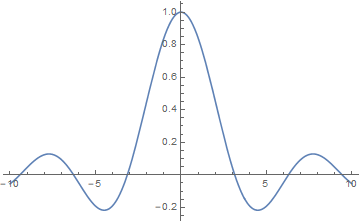
\includegraphics[scale=1]{fourier_1.png}
	\end{figure}
\end{exmp}

$\,$\\

\begin{exmp}
 	Let 
 	\begin{align*}
 	f(x) =
 	\begin{cases}
 	e^{-x}, \hspace{0.5cm} x\geq 0\\
 	e^{x}, \hspace{0.5cm} x < 0.
 	\end{cases}
 	\end{align*}	
 	Then
 	\begin{align*}
 	\hat{f}(\xi) &= \frac{1}{\sqrt{2\pi}}\left(\int^\infty_0 e^{-(x+i\xi)}\,dx + \int^\infty_0 e^{-x + i\xi x}\,dx \right)\\
 	&= \frac{1}{\sqrt{2\pi}}\left(\int^\infty_0 e^{-x(1+i\xi)} - e^{-x(1-i\xi)}\,dx\right)\\
 	&= \frac{-1}{\sqrt{2\pi}}\left(-\frac{1}{1+i\xi} + \frac{1}{1-i\xi}\right)\\
 	&= \frac{1}{2\pi}\frac{-2i\xi}{1+\xi^2}\\
 	&= -i\sqrt{\frac{2}{\pi}}\frac{\xi}{1+\xi^2}.
 	\end{align*}
 	\begin{figure}[h!]
 		\centering
 		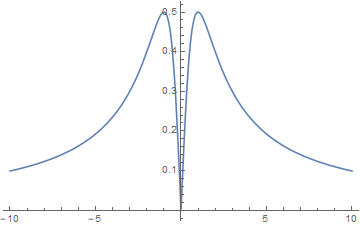
\includegraphics[scale=1]{fourier_2.png}
 	\end{figure}
\end{exmp}



\newpage


\begin{exmp}
	Consider the Gaussian function
	\begin{align*}
	f(x) = e^{-x^2}
	\end{align*}
	then we can show
	\begin{align*}
	\hat{f}(\xi) = \frac{1}{\sqrt{2}}e^{-(\xi/2)^2}.
	\end{align*}
	We say that the Gaussian function is in some sense the ``eigenfunction'' of the Fourier Transform.
\end{exmp}
$\,$\\

\begin{prop}
	\begin{align*}
	\sqrt{\pi} = \int^\infty_{-\infty}e^{-x^2}\,dx.
	\end{align*}
	
	\begin{proof}
		\begin{defn}
			\begin{align*}
			I = \int^\infty_{-\infty}e^{-x^2}\,dx = \int^\infty_{-\infty}e^{-y^2}\,dy\\
			\end{align*}
			So
			\begin{align*}
			I^2 = \left(\int^\infty_{-\infty}e^{-x^2}\,dx\right)\left(\int^\infty_{-\infty}e^{-y^2}\,dy\right).
			\end{align*}
			So,
			\begin{align*}
			I^2 = \iint_{\mathbb{R}}e^{-(x^2+y^2)\,dxdy}
			\end{align*}
			We change into polar coordinate
			\begin{align*}
			0 \leq r \leq \infty\\
			0 \leq \theta \leq 2\pi.
			\end{align*}
			So
			\begin{align*}
			I^2 = \int^\infty_0 \int^{2\pi}_0 e^{-r^2}r\,d\theta dr = -\pi\int^\infty_{-\infty}2re^{-r^2}\,dr = -\pi.
			\end{align*}
		\end{defn}
	\end{proof}
	
\end{prop}


$\,$\\


We have seen that 
\begin{enumerate}
	\item $\F$ is a linear map.
	\item $\F[f'](\xi) = i\xi \F[f](\xi)$
	\item $\F[f''](\xi) = -\xi^2 \F[f](\xi)$.
\end{enumerate}

But $\widehat{fg} \neq \hat{f}\hat{g}$. Though this pointwise product isn't preserved under the Fourier Transform, another product is the \textbf{Convolution Product}:

\begin{defn}
	Given ``nice'' $g,f : \mathbb{R} \to \mathbb{R}$. The convolution of $f$ and $g$, denoted by $f\ast g : \mathbb{R} \to \mathbb{R}$ defined by
	\begin{align*}
	(f\ast g)(x) = \frac{1}{\sqrt{2\pi}}\int^\infty_{-\infty}f(y)g(x-y)\,dy.
	\end{align*}
\end{defn}

\begin{prop}
	\begin{align*}
	f\ast g = g \ast f.
	\end{align*}
\end{prop}

\begin{exmp}
	\begin{align*}
	f(x) = x \hspace{0.5cm} g(x) = e^{-x^2}.
	\end{align*}
	Then
	\begin{align*}
	(f\ast g)(x) &= \frac{1}{\sqrt{2\pi}}\int^\infty_{-\infty}e^{-y^2}(x-y)\,dy\\
	&= \frac{x}{\sqrt{2\pi}}\sqrt{\pi}\\
	&= \frac{x}{\sqrt{2}}.
	\end{align*}
\end{exmp}

\begin{thm}
	 For $f,g$ ``nice'' enough,
	\begin{align*}
	\F[f\ast g](\xi) = \hat{f}(\xi)\hat{g}(\xi)
	\end{align*}
	\begin{proof}
		\begin{align*}
		\F[f\ast g] &= \frac{1}{\sqrt{2\pi}}\int^\infty_{-\infty}(f\ast g)(x)e^{-i x \xi}\,dx\\
		&= \frac{1}{\sqrt{2\pi}}\int^\infty_{-\infty}\left(\frac{1}{\sqrt{2\pi}}  \int^\infty_{-\infty}f(y)g(x-y)\,dy \right)e^{-i x \xi}\,dx\\
		&= \frac{1}{2\pi}\int^\infty_{-\infty}\int^\infty_{-\infty}f(y)g(x-y)e^{-i(x-y)\xi}e^{-iy\xi}\,dydx\\
		&= 
		\frac{1}{2\pi}\int^\infty_{-\infty}f(y)e^{-iy\xi}\int^\infty_{-\infty}g(x-y)e^{-i(x-y)\xi}\,dxdy,
		\end{align*}
		where the last line comes from Fubini's theorem. Change of variables: $u=x-y$:
		\begin{align*}
		\F[f\ast g] = \hat{g}(\xi)\hat{f}(\xi).
		\end{align*}
	\end{proof}
\end{thm}





% Mar 18, 2019%


%\newcommand{\o}{\omega}
%
%
%\newcommand{\f}[2]{\frac{#1}{#2}}
%
%\newcommand{\ift}{\infty}
%
%\newcommand{\lp}{\left(}
%\newcommand{\rp}{\right)}
%
%\newcommand{\lb}{\left[}
%\newcommand{\rb}{\right]}
%
%\newcommand{\lc}{\left\{}
%\newcommand{\rc}{\right\}}
%\newcommand{\w}{\omega}
%\newcommand{\lam}{\lambda}
%\newcommand{\al}{\alpha}
%\newcommand{\b}{\beta}
%\newcommand{\x}{\xi}




\begin{align}
\ift\lp \lb\lc\f{hello}{goodbye}\rc\rb \rp \\
\exp(hello)\\
\w\\
\lam\\
\al\\
\be\\
\x
\end{align}


























































































































\newpage

\section{Problems and Solutions}
\subsection{Problem set 1}
\begin{exer*}
	\begin{prob*}2, Lesson 2.
		The heat equation is
		\begin{align*}
		u_t = \alpha^2 u_{xx} + 1, \text{ with }0 < x < 1.
		\end{align*}
		Suppose $u(0,t) = 0$ and $u(1,t) = 1$. What is the steady-state temperature of the rod?\\
		\begin{sln*}
			Stead-state temperature can be found by setting $u_t(x,t) = 0$ for $0 < x < 1$. It follows that $\alpha^2 u_{xx}(x,t) + 1 = 0$. In addition, the temperature profile is no longer time-dependent, so $u(x,t)\to u(x)$. These conditions give
			\begin{align*}
			u_{xx}(x) &= -\frac{1}{\alpha^2}\\
			u(x) &= -\frac{1}{2\alpha^2}x^2 + Cx + D.
			\end{align*} 
			Applying the boundary conditions $u(0,t)=0$ and $u(1,t)=1$, we can find $C$ and $D$:
			\begin{align*}
			\begin{cases}
			u(0) = 0 = D\\
			u(1) = -\frac{1}{2\alpha^2} + C = 1
			\end{cases}.
			\end{align*}
			So, $C = 1 + 1/s\alpha^2$. The temperature profile of the rod is then
			\begin{align*}
			u_{\text{steady-state}}(x) = -\frac{1}{2\alpha^2}x^2 + \left(1 + \frac{1}{2\alpha^2} \right)x .
			\end{align*}
		\end{sln*}
	\end{prob*}
	
	\newpage
	
	\begin{prob*}3, Lesson 2. The heat equation is
		\begin{align*}
		u_t = \alpha^2 u_{xx} - \beta u, \text{ with } 0<x<1.
		\end{align*}
		Suppose the BC is $u(0,t)=1$ and $u(1,t)=1$. What is the steady-state temperature of the rod?\\
		\begin{sln*}
			Again, we set $u_t = 0$ to find the steady-state temperature profile. This forces $\alpha^2 u_{xx} - \beta u = 0$, i.e., $\alpha^2 u_{xx} = \beta u$. Next, since the temperature is no longer time-dependent, we can let $u(x,t)\to u(x)$. Now, because $\beta$ and $\alpha^2$ are both positive numbers, the solution to this ODE has the form
			\begin{align*}
			u_{\text{steady-state}} = u(x) = Ce^{-\sqrt{\frac{\beta}{\alpha^2}}x} + De^{\sqrt{\frac{\beta}{\alpha^2}}x}.
			\end{align*}
			Let us denote $\sqrt{\beta/\alpha^2}$ as $\phi$. To find the coefficients $C$ and $D$, we apply the boundary condition:
			\begin{align*}
			\begin{cases}
			u(0) = C + D = 1\\
			u(1) = Ce^{-\phi} + De^{\phi} = 1.
			\end{cases}
			\end{align*}
			Solving this linear system of equation in Mathematica we find 
			\begin{align*}
			C &= \frac{e^\phi}{1 + e^\phi}\\
			D &= \frac{1}{1+e^\phi}.
			\end{align*}
			So, the steady-state temperature profile is
			\begin{align*}
			u_s(x) =  \frac{e^\phi}{1 + e^\phi}e^{-\phi x} + \frac{1}{1+e^\phi}e^{\phi x} = \frac{1}{1+e^\phi}\left( e^{\phi(1-x)} + e^{\phi x} \right),
			\end{align*}
			where
			\begin{align*}
			\phi = \sqrt{\frac{\beta}{\alpha^2}}.
			\end{align*}
			Mathematica code and graph of steady-state temperature distribution:
			\begin{figure}[h!]
				\centering
				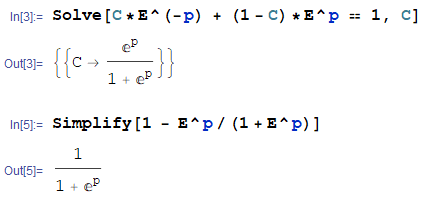
\includegraphics[scale=0.5]{1.png}
			\end{figure}
			\begin{figure}[h!]
				\centering
				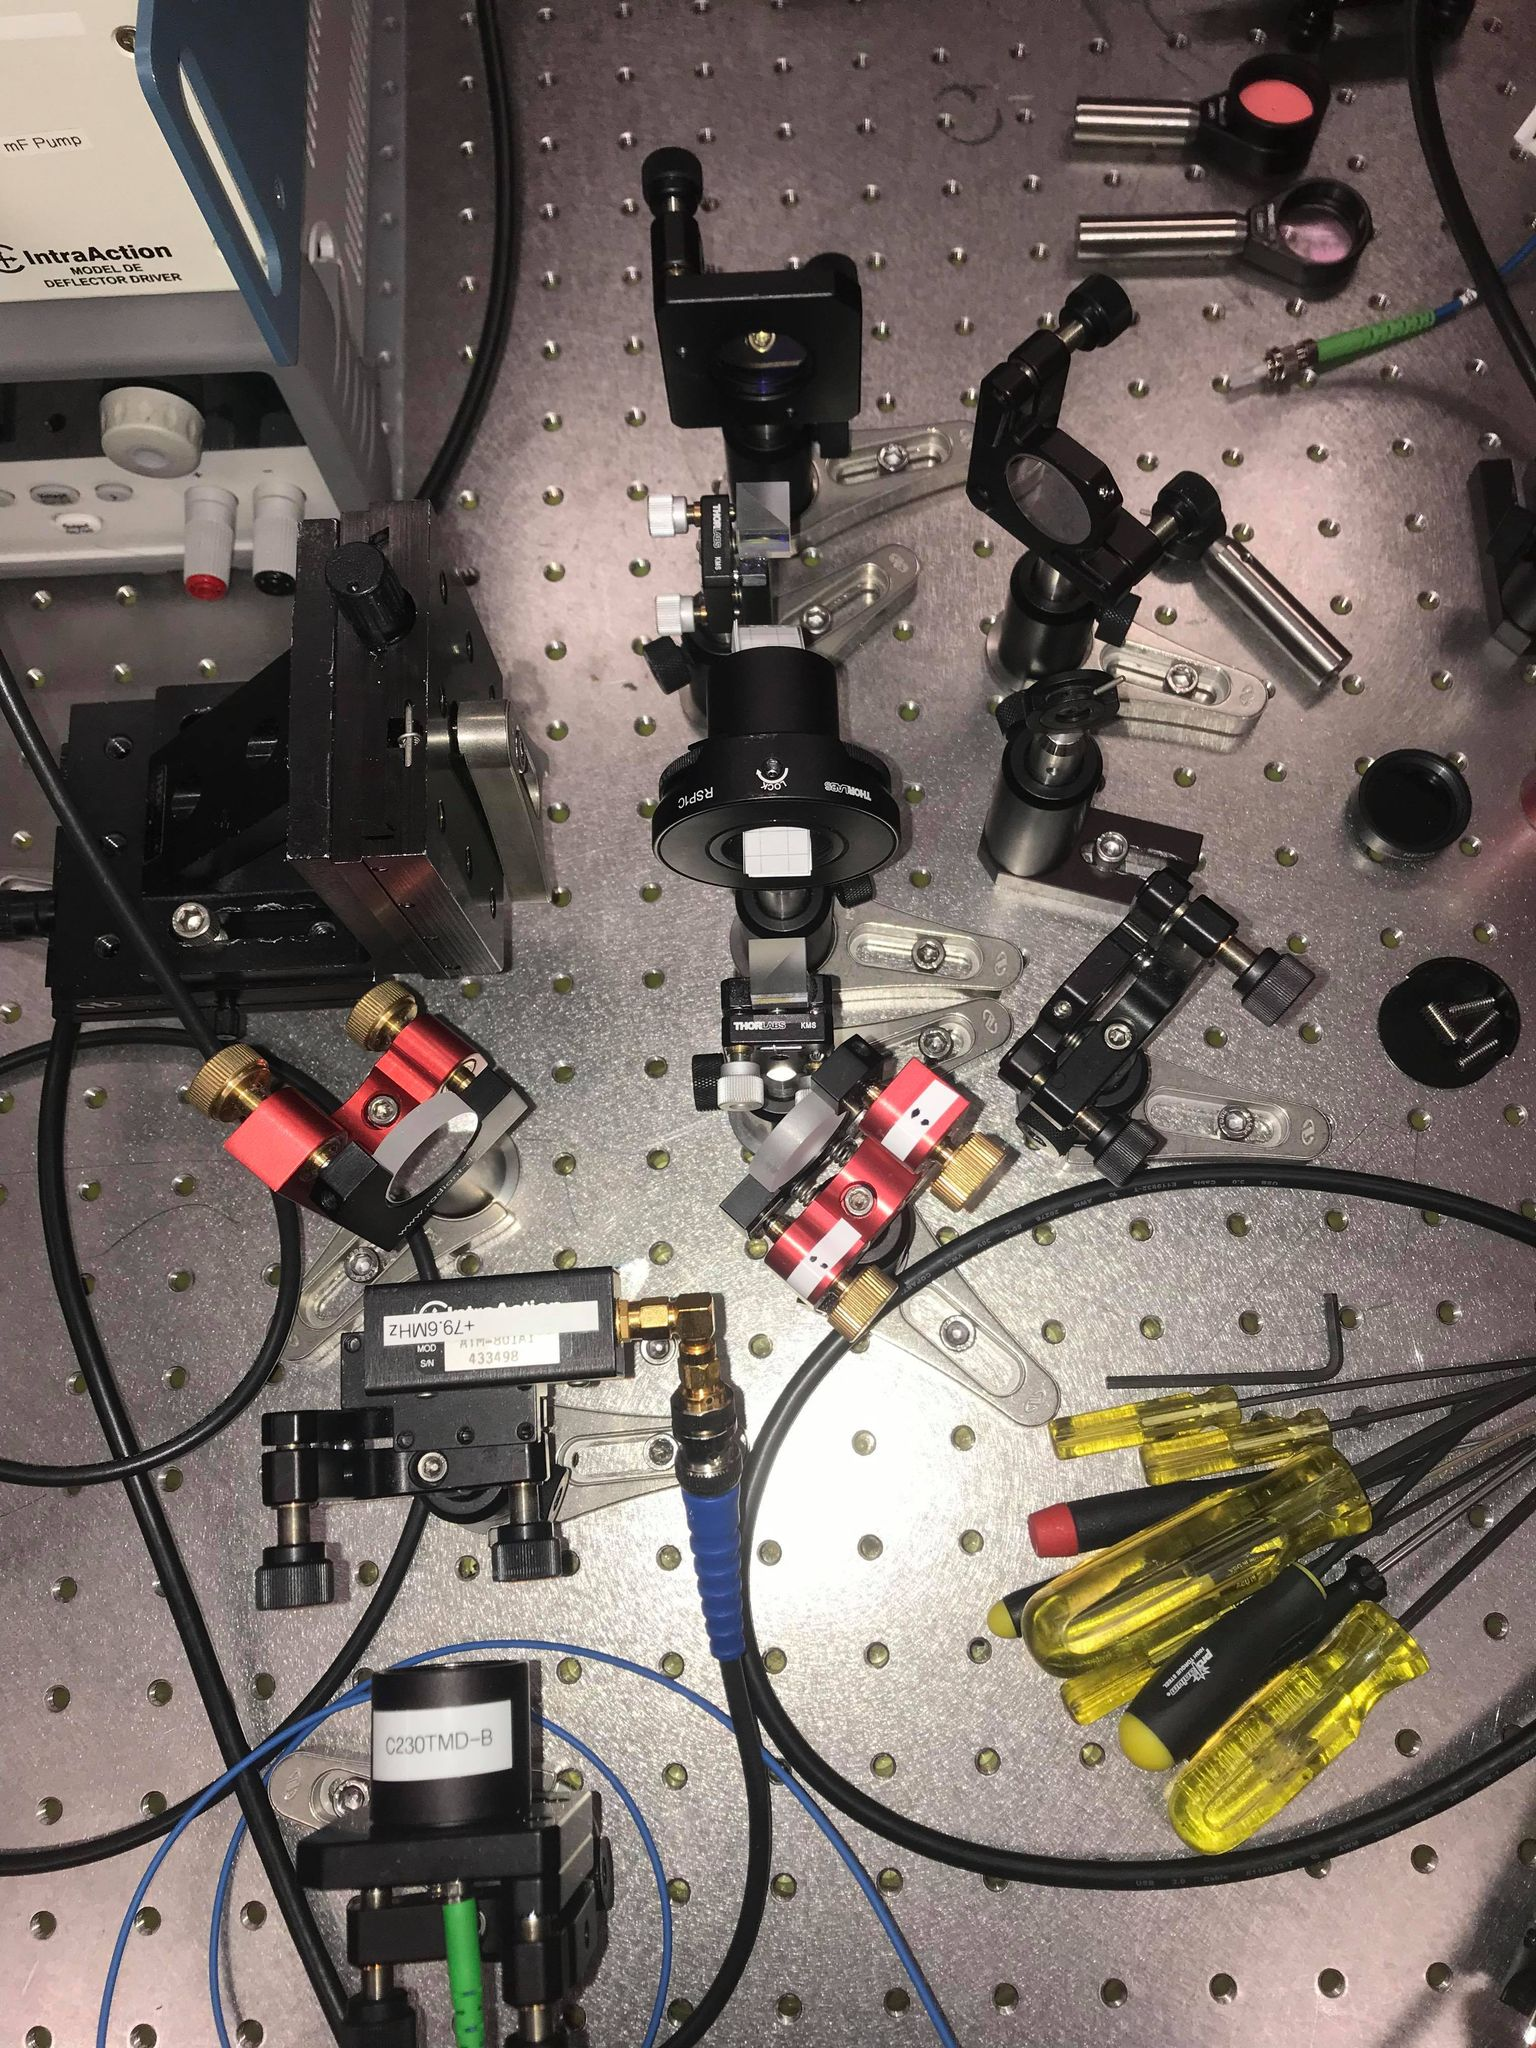
\includegraphics[scale=0.5]{2.png}
			\end{figure}
		\end{sln*}
	\end{prob*}
\end{exer*}

\newpage


\begin{exer*}
	\begin{prob*}1, Lesson 3. Sketch the solution to the IBVP (Farlow, 3.6) for different values of time. Check if they agree with the boundary conditions. What is the steady-state temperature of the rod? Is this obvious?\\
		
		The IBVP:
		\begin{align*}
		\begin{cases}
		PDE: u_t = \alpha^2 u_{xx}, x\in(0,200), t\in(0,\infty)\\
		BC_1: u_x(0,t) = 0, t\in(0,\infty)\\
		BC_2: u_x(200,t) = -\frac{h}{k}[u(200,t) - 20], t\in(0,\infty)\\
		IC: u(x,0) = 0, x\in[0,200]
		\end{cases}
		\end{align*}
		\begin{sln}
			Sketches:\\\\\\\\\\\\\\\\\\\
			
			Intuitively, the steady-state temperature of the rod is just 20$^\circ$C, since the rod in the problem, which is initially at 0$^\circ$C, is simply being warmed up by the 20$^\circ$C water. We can of course show this mathematically. By the steady-state condition, $u_t = 0 = u_{xx}$. This forces $u_{xx} = Cx + D$. But by the first boundary condition $u_x(0,t)=0$, require that $C = 0$. The second boundary condition requires that $u_{s,x} = C = 0 = (-h/k)[u(200,t) -20] = (-h/k)[200C + D - 20]$, which means $D=20$. So, the steady-state temperature profile, not surprisingly, is 20$^\circ$C uniform along the length of the rod. 
		\end{sln}
	\end{prob*}
	\newpage
	\begin{prob*}2, Lesson 3. Interpret the IBVP:
		\begin{align*}
		\begin{cases}
		PDE: u_t = \alpha^2 u_{xx}, x\in(0,1), t\in(0,\infty)\\
		BC_1: u(0,t) = 0, t\in(0,\infty)\\
		BC_2: u_x(1,t) = 1, t\in(0,\infty)\\
		IC: u(x,0) = \sin(\pi x), x\in[0,1]
		\end{cases}
		\end{align*}
		\begin{sln}
			$\,$\\
			
			\textit{Interpretation:} The PDE suggests that we are dealing with heat flow in one dimension, so we can imagine a rod of length 1 with no laterally heat transfer. The first boundary condition suggests that the temperature is held fixed at 0 at $x=0$ for all $t$. The second boundary condition suggests that temperature is increasing (at a constant rate) at $x=1$ end. The initial condition tells us that initially, the temperature profile of the rod has a sinusoidal distribution across the rod's length, with the ends having temperature of 0 ($\sin(0)=\sin(\pi) = 0$) and the middle $x=1/2$ having the highest temperature of 1. \\
			
			\textit{Steady-state?} The steady-state condition requires that $u_{xx} = 0$, so again, we have $u_s(x) = Cx +D$, where $C,D$ are real constants. The first boundary condition requires $D=0$. The second boundary condition requires that $u_x(1) = C\times 1 = C = 1$. Therefore, in the long run, $u_s(x) = x$. So, the stead-state temperature at each point of the rod has the same value as the position (from the 0 degree end) of that point on the rod. \\
			
			\textit{Sketches:}
		\end{sln}
	\end{prob*}
	\newpage
	\begin{prob*}3, Lesson 3. Interpret the following IBVP:
		\begin{align*}
		\begin{cases}
		PDE: u_t = \alpha^2 u_{xx}, x\in(0,1), t\in(0,\infty)\\
		BC_1: u_x(0,t) = 0, t\in(0,\infty)\\
		BC_2: u_x(1,t) = 0, t\in(0,\infty)\\
		IC: u(x,0) = \sin(\pi x), x\in[0,1]
		\end{cases}
		\end{align*}
		\begin{sln}
			$\,$\\
			
			\textit{Interpretation:} The PDE suggests that we are dealing with heat flow in one dimension, so we can imagine a rod of length 1 with no laterally heat transfer. The boundary conditions suggest that there are no temperature gradients at the ends of the rod. So we imagine the rod being insulated at the ends. The initial condition is like that in the previous problem where the temperature profile of the rod has a sinusoidal distribution across the rod's length, with the ends being at zero degrees ($\sin(0)=\sin(\pi) = 0$) and the middle $x=1/2$ having the highest temperature of 1. \\
			
			\textit{Steady-state:} The steady-state condition requires that $u_{xx} = 0$, i.e., $u_s(x) = Cx + D$, where $C,D$ are real constants. Since the temperatures are fixed at the end points, $u_{s,x} = C = 0$. So the steady state temperature is $D$, which takes some value between 0 and 1 as $t\to \infty$. The steady-state temperature profile is the same along the length of the rod. \\
			
			\textit{Sketches:}
		\end{sln}
	\end{prob*}
\end{exer*}

\newpage


\begin{exer*}
	\begin{prob*}3, Lesson 4. Derive the heat equation
		\begin{align*}
		u_t = \frac{1}{c\rho}\p_x[k(x)u_x] + f(x,t)
		\end{align*}
		for the situation where the thermal conductivity $k(x)$ depends on $x$.\\
		\begin{sln*}
			We can start the derivation from step (4.2) in Farlow's, modify $k \to k(x)$. The conservation of energy gives:
			\begin{align*}
			c\rho A\int_{x}^{x+\Delta x}u_t(s,t)\,ds = A\left(k(x+\Delta x)u_x(x+\Delta x,t) - k(x)u_x(x,t)  + \int_x^{x+\Delta x}f(s,t)\,ds \right).
			\end{align*}
			By the MVT, there exists $\zeta \in (x,x+\Delta x)$ such that
			\begin{align*}
			c\rho u_t(\zeta, t)\Delta x = k(x+\Delta x)u_x(x+\Delta x,t) - k(x)u_x(x,t) + f(\zeta,t)\Delta x,
			\end{align*} 
			i.e.,
			\begin{align*}
			u_t(\zeta,t) &= \frac{1}{c\rho}\left\{ \frac{k(x+\Delta x)u_x(x+\Delta x,t) - k(x)u_x(x,t)}{\Delta x} \right\} + \frac{1}{c\rho}f(\zeta,t)
			\end{align*}
			Letting $\Delta x \to 0$, we turn the term with $\Delta x$ into a derivative of a composition defined as $UK(x,t) = k(x)u_x(x,t)$. The result is
			\begin{align*}
			u_t(x,t) = \frac{1}{c\rho}\p_x(k(x)u_x(x,t)) + f(x,t),
			\end{align*}
			where we simply let $f(x,t)$ absorb the constant $(c\rho)^{-1}$. We have obtained the heat equation with $x$-dependent thermal conductivity. 
		\end{sln*}
	\end{prob*}
\end{exer*}

\newpage

\begin{exer*}
	\begin{prob*}1, Lesson 5. Show that
		\begin{align*}
		u(x,t) = e^{-\lambda^2\alpha^2 t}(A\sin\lambda x + B\cos \lambda x)
		\end{align*}
		satisfies the PDE $u_t = \alpha^2 u_{xx}$ for $A,B,\lambda \in \R$.
		\begin{sln*}
			We can compute the partial derivatives and verify that $u(x,t)$ solves the PDE ``by inspection.'' The $t$-derivative gives the same $u(x,t)$, multiplied by a factor of $-\lambda^2\alpha^2$, while the $x$-second derivative also gives $u(x,t)$, but multiplied by factor of $\lambda^2$. So, these expressions differ by a factor of $\alpha^2$.  Mathematically:
			\begin{align*}
			u_t = -\lambda^2 \alpha^2 u(x,t) = \alpha^2 u_{xx}.
			\end{align*}
			Hence, $u(x,t)$ solves the given PDE. 
		\end{sln*}
	\end{prob*}
	\newpage
	\begin{prob*}2, Lesson 5. Let $\delta^m_n$ denotes the Kronecker delta, where $m,n$ are non-negative whole numbers. Show
		\begin{align*}
		\int_{0}^{1}\sin(\pi mx)\sin(\pi nx)\,dx = \frac{1}{2}\delta^m_n
		\end{align*}
		\begin{sln*}
			Applying the hinted trigonometric identity, we have
			\begin{align*}
			\int_{0}^{1}\sin(\pi mx)\sin(\pi nx)\,dx &= \frac{1}{2}\int_0^1\cos[(m-n)\pi x] - \cos[(m+n)\pi x]\,dx\\
			&= \frac{1}{2}\int_0^1\cos[(m-n)\pi x]\,dx - \frac{1}{2}\int_0^1\cos[(m+n)\pi x]\,dx
			\end{align*}
			At this point, we can argue why the equality given by the problem is true without much computation. The argument goes as follows. If $m = n$, then the second integral vanishes because $\cos(xk\pi)$, where $k$ is an even number and $x\in [0,1]$, is symmetric about $x=1/2$ and $y=0$. If $m\neq n$, then $m-n$ and $m+n$ are either odd or even. If they are even (and positive), then both integrals on the right hand side vanish. If they are odd, then we can assume (without loss of generality) that $m$ is odd and $n$ is even. This makes $\sin(\pi m x)\sin(\pi n x)$ symmetric about $x=1/2$ and $y=0$, so the integral also vanishes over $x\in[0,1]$.
		\end{sln*}
	\end{prob*}
	\newpage
	\begin{prob*}5, Lesson 5. What is the solution to problem 4 in Farlow, Lesson 5 (which also requires doing 3) if the initial condition is changed to 
		\begin{align*}
		u(x,0) = \sin(2\pi x) + \frac{1}{3}\sin(4\pi x) + \frac{1}{5}\sin(6\pi x)
		\end{align*}
		\begin{sln*}
			We should quickly do problem 3 first. If $\Phi(x) = 1$, $x\in[0,1]$. Applying the formula for the coefficients $A_n$:
			\begin{align*}
			A_n = 2\int_0^1\Phi(x)\sin(n\pi x)\,dx = 2\int_0^1\sin(n\pi x)\,dx = \frac{2}{n\pi}(1-\cos(n\pi x)) = \begin{cases}
			\frac{4}{n\pi}, n \text{ odd}\\
			0, n\text{ even}
			\end{cases}.
			\end{align*}
			So, the Fourier expansion for $\Phi(x) = 1$ is
			\begin{align*}
			\Phi(x) =1 = \frac{4}{\pi}\left[\sin(\pi x) + \frac{1}{3}\sin(3\pi x) + \frac{1}{5}\sin(5\pi x)+\dots \right].
			\end{align*}
			In problem 4, the boundary and initial conditions suggests using $\Phi(x)$ from problem 3. So, given the formula for $u(x,t)$, we simply substitute in the coefficients to generate a Fourier expansion for $u(x,t)$:
			\begin{align*}
			u(x,t) &= \sum_{n=1}^{\infty}A_n e^{-(n\pi)^2t}\sin(n\pi x)\\
			&= \frac{4}{\pi}\left[ e^{-(\pi)^2t}\sin(\pi x) + \frac{1}{3}e^{-(3\pi)^2t}\sin(3\pi x)
			+ \frac{1}{5}e^{-(5\pi)^2t}\sin(5\pi x)+\dots\right].
			\end{align*}
			Back to problem 5, if the initial condition is given as $u(x,0)$ above, then we might think we have to re-do and find a new Fourier expansion. But by inspecting the form of $u(x,0)$, we can see that it is just a truncated Fourier expansion. So there is no need to find the coefficients $A_n$ since they are already given to us. So, carefully picking out the coefficients, we get the new solution
			\begin{align*}
			u(x,t) = e^{-(2\pi)^2t}\sin(2\pi x) + \frac{1}{3}e^{-(4\pi)^2t}\sin(4\pi x) + \frac{1}{5}e^{-(6\pi)^2t}\sin(6\pi x).
			\end{align*}
		\end{sln*}
	\end{prob*}
\end{exer*}

\newpage
\subsection{Problem set 2}


\begin{exer*}\textbf{Problem 2, Lesson 6}
	
	\noindent Transform
	\begin{align*}
	&PDE: u_t = u_{xx},\,\,\,\,\,\,\,\,\,\,\, 0<x<1\\
	&BCs:  
	\begin{cases}
	u(0,t) = 0\\
	u(1,t) = 1
	\end{cases} 0 < t < \infty\\
	&IC: u(x,0) = x^2,\,\,\,\,\,\,\,\,\,\,\, 0 \leq x\leq 1
	\end{align*}
	to zero BCs and solve the new problem. What will the solution to this problem look like for different values of time? Does the solution agree with your intuition? What is the steady-state solution? What does the transient solution look like?
	\begin{sln*}
		$\,$\\
		Let $u(x,t) = U(x,t) + S(x,t)$ where $U(x,t)$ is the transient solution while $S(x,t)$ is the steady-state solution to the IBVP. To find the steady-state solution $S(x,t)$, we set $u_t = 0$ and $U(x,t) = 0$. Applying the boundary conditions, we find 
		\begin{align*}
		S(x,t) = S(x) = Cx+D = x.
		\end{align*}
		So,
		\begin{align*}
		u(x,t) = x + U(x,t).
		\end{align*}
		Since $u_t = U_t$ and $u_{xx} = U_{xx}$, we can re-write the origin IBVP as
		\begin{align*}
		&PDE: U_t = U_{xx},\,\,\,\,\,\,\,\,\,\,\, 0<x<1\\
		&BCs:  
		\begin{cases}
		U(0,t) = 0\\
		U(1,t) = 0
		\end{cases} 0 < t < \infty\\
		&IC: U(x,0) = x^2 - x,\,\,\,\,\,\,\,\,\,\,\, 0 \leq x\leq 1
		\end{align*}
		The solution $U(x,t)$ to this IBVP is given by
		\begin{align*}
		U(x,t) = \sum^\infty_{n=1}A_n e^{-(n\pi)^2t} \sin(n\pi x),
		\end{align*}
		where
		\begin{align*}
		A_n = 2\int_{0}^{1}(x^2 - x)\sin(n\pi x)\,dx &= 2\frac{-2+2\cos(n\pi) + n\pi\sin(n\pi)}{n^3\pi^3}\\
		&= \begin{cases}
		\frac{-8}{n^3\pi^3},\,\,\,\,\, n \text{ odd}\\
		0,\,\,\,\,\,\,\,\,\, n \text{ even}.
		\end{cases}.
		\end{align*}
		The second equality comes from integrating in Mathematica, which can also be done with integration by parts. The transient solution is then
		\begin{align*}
		U(x,t) = -\frac{8}{\pi ^3}e^{-(\pi)^2t} \sin(\pi x)   -\frac{8}{27 \pi ^3}e^{-(3\pi)^2t} \sin(3\pi x)    -\frac{8}{125 \pi ^3}e^{-(5\pi)^2t} \sin(5\pi x)  + \dots
		\end{align*}
		The full solution to the IBVP is
		\begin{align*}
		u(x,t) &= x- \frac{8}{\pi^3}\sum_{n=1}^\infty\frac{1}{n^3}e^{-(n\pi)^2t}\sin(n\pi x),\,\,\, n \text{ odd} \\ 
		&= x -\frac{8}{\pi ^3}e^{-(\pi)^2t} \sin(\pi x)   -\frac{8}{27 \pi ^3}e^{-(3\pi)^2t} \sin(3\pi x)    -\frac{8}{125 \pi ^3}e^{-(5\pi)^2t} \sin(5\pi x)  + \dots
		\end{align*}
		
		\newpage
		
		\noindent Mathematica code:
		\begin{lstlisting}
		In[6]:= Simplify[Integrate[(x^2 - x) Sin[n*Pi*x], {x, 0, 1}]]
		
		Out[6]= (-2 + 2 Cos[n \[Pi]] + n \[Pi] Sin[n \[Pi]])/(n^3 \[Pi]^3)
		
		In[4]:= F[n_] := Simplify[Integrate[(x^2 - x) Sin[n*Pi*x], {x, 0, 1}]]
		
		In[7]:= Table[F[n], {n, 1, 10}]
		
		Out[7]= {-(4/\[Pi]^3), 0, -(4/(27 \[Pi]^3)), 0, -(4/(
		125 \[Pi]^3)), 0, -(4/(343 \[Pi]^3)), 0, -(4/(729 \[Pi]^3)), 0}
		\end{lstlisting}
		$\,$\\
		\noindent Solutions for different values of time:\\
		
		\begin{figure}[h!]
			\centering
			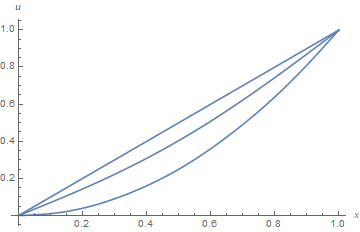
\includegraphics[scale=0.7]{pset2_1.png}
		\end{figure}
		
		\noindent Mathematica code:
		\begin{lstlisting}
		U[x_, t_] := 
		x - (8 E^(-\[Pi]^2 t) Sin[\[Pi] x])/\[Pi]^3 - (
		8 E^(-9 \[Pi]^2 t) Sin[3 \[Pi] x])/(27 \[Pi]^3) - (
		8 E^(-25 \[Pi]^2 t) Sin[5 \[Pi] x])/(125 \[Pi]^3)
		
		Show[Plot[U[x, 0], {x, 0, 1}], Plot[U[x, 0.1], {x, 0, 1}], 
		Plot[U[x, 1], {x, 0, 1}]]
		\end{lstlisting}
		
		The solution matches my intuition. The IBVP simply states that the temperature at the ends are fixed, and that the temperature is initially distributed across the rod as $x^2$. Since the temperatures at the ends are fixed it is expected that in the long run the temperature increases uniformly across the rod, in agreement with the steady-state solution. 
		
	\end{sln*}
\end{exer*}
\newpage






\begin{exer*}\textbf{Problem 3, Lesson 6}
	Transform
	\begin{align*}
	&PDE: u_t = u_{xx},\,\,\,\,\,\,\,\,\,\,\, 0<x<1\\
	&BCs:  
	\begin{cases}
	u_x(0,t) = 0\\
	u_x(1,t) + hu(1,t)= 1
	\end{cases} 0 < t < \infty\\
	&IC: u(x,0) = \sin(\pi x),\,\,\,\,\,\,\,\,\,\,\, 0 \leq x\leq 1
	\end{align*}
	into a new problem with zero BCs. Is the new PDE homogeneous?
	
	\begin{sln*}
		$\,$\\
		
		Once again, we let $u(x,t) = U(x,t) + S(x,t)$ where $S(x,t)$ is the steady-state solution. $S(x,t)$ has the form:
		\begin{align*}
		S(x,t) = A(t)\left( 1 - \frac{x}{L} \right) + B(t)\left( \frac{x}{L} \right) = A(t)\left( 1 - x \right) + B(t)\left( x \right),
		\end{align*} 
		where
		\begin{align*}
		S(0,t) &= A(t)\\
		S(1,t) &= B(t)\\
		S_x(0,t) &= B(t) - A(t) = S_x(1,t).
		\end{align*}
		Applying the boundary conditions,
		\begin{align*}
		\begin{pmatrix}
		-1 & 1\\
		-1 & h + 1
		\end{pmatrix}
		\begin{pmatrix}
		A(t) \\ B(t)
		\end{pmatrix}
		=
		\begin{pmatrix}
		0\\1
		\end{pmatrix}
		\end{align*} 
		Solving the system for $A(t)$ and $B(t)$ gives
		\begin{align*}
		A(t) = B(t) = \frac{1}{h}
		\end{align*}
		So, the steady-state solution is
		\begin{align*}
		S(x,t) = \frac{1}{h}(1-x+x) = \frac{1}{h},
		\end{align*}
		which is independent of $t$ and $x$. Therefore, $u_t = U_t = u_{xx} = U_{xx}$. Applying the initial condition, we find 
		\begin{align*}
		u(x,0) = S(x,0) + U(x,0) = \frac{1}{h} + U(x,0) = \sin(\pi x)
		\end{align*}
		and
		\begin{align*}
		u_x(1,t) + hu(1,t) = U(1,t) + hU(1,t) + \frac{h}{h} = 1.
		\end{align*}
		So, the new IBVP is:
		\begin{align*}
		&PDE: U_t = U_{xx},\,\,\,\,\,\,\,\,\,\,\, 0<x<1\\
		&BCs:  
		\begin{cases}
		U_x(0,t) = 0\\
		U_x(1,t) + hU(1,t)= 0
		\end{cases} 0 < t < \infty\\
		&IC: u(x,0) = \sin(\pi x)-\frac{1}{h}   ,\,\,\,\,\,\,\,\,\,\,\, 0 \leq x\leq 1
		\end{align*}
		We notice that the new PDE is still homogeneous. 
	\end{sln*}
\end{exer*}
\newpage









\begin{exer*}\textbf{Problem 1, Lesson 7}
	Solve the following heat-flaw problem:
	\begin{align*}
	&PDE: u_t = u_{xx},\,\,\,\,\,\,\,\,\,\,\, 0<x<1, 0<t<\infty\\
	&BCs:  
	\begin{cases}
	u(0,t) = 0\\
	u_x(1,t) = 0
	\end{cases} 0 < t < \infty\\
	&IC: u(x,0) = x,\,\,\,\,\,\,\,\,\,\,\, 0 \leq x\leq 1
	\end{align*}
	by separation of variables. Does your solution agree with the your intuition? What is the steady-state solution? 
	\begin{sln*}
		$\,$\\
		
		\noindent By separation of variables, we assume $u(x,t) = T(t)X(x)$. By the PDE, 
		\begin{align*}
		\frac{T'(t)}{T(t)} = \frac{X''(x)}{X(x)} = \mu,
		\end{align*}
		where $\mu$ is some constant. We reject solutions with $\mu > 0$ on physical grounds. If $\mu = 0$, then $T'(t) = X''(x) = 0$, so
		\begin{align*}
		u(x,t) = Ax + B.
		\end{align*}
		To satisfy the boundary conditions:
		\begin{align*}
		u(0,t) &= B = 0\\
		u_x(1,t) &= A = 0.
		\end{align*}
		This $u(x,t) = 0$, a trivial solution. If $\mu < 0$, then we let $\mu = -\lambda^2$. We immediately have
		\begin{align*}
		T(t) &= Ae^{-\lambda^2 t}\\
		X(x) &= C\sin(\lambda x) + B\cos(\lambda x).
		\end{align*}
		So, the general solution is
		\begin{align*}
		u(x,t) = e^{-\lambda^2 t}(A\sin(\lambda x) + B\cos(\lambda x)).
		\end{align*}
		Subjecting $u(x,t)$ to the first boundary condition, we find $B = 0$, which reduces the solution to
		\begin{align*}
		u(x,t) = Ae^{-\lambda^2 t}\sin(\lambda x).
		\end{align*}
		The second boundary condition gives
		\begin{align*}
		A\cos(\lambda)= 0.
		\end{align*}
		Assuming $A\neq 0$, so that our solution is not trivial, 
		\begin{align*}
		\lambda = \frac{k\pi}{2},\,\,\,\,\,\,\,\, k \text{ odd}.
		\end{align*}
		The solution is then
		\begin{align*}
		u(x,t) = \sum_{k=1}^{\infty}A_ke^{-(k\pi/2)^2t}\sin\left(\frac{k\pi}{2} x\right), \,\,\, k \text{ odd}.
		\end{align*}
		To find the coefficients $A_k$, we invoke Fourier's trick, for odd $n$'s:
		\begin{align*}
		\int_{0}^1 u_0(x)\sin\left(\frac{n\pi}{2} x\right)\,dx &= \int_0^1 \sin\left(\frac{n\pi}{2} x\right)\sum_{k=1}^\infty A_k\sin\left(\frac{k\pi}{2} x\right)\,dx\\
		&= \sum_{k=1}^\infty A_k \int_{0}^1 \sin\left(\frac{n\pi}{2} x\right)\sin\left(\frac{k\pi}{2} x\right)\,dx\\
		&= \sum_{k=1}^\infty \frac{1}{2}A_k\delta^k_n\\
		&= \frac{1}{2}A_n.
		\end{align*}
		So,
		\begin{align*}
		A_k = 2\int_{0}^1x\sin\left(\frac{k\pi}{2} x\right)\,dx,\,\,\,\, k \text{ odd}.
		\end{align*}
		So, the transient solution has the form:
		\begin{align*}
		U(x,t) &= \sum_{k=1}^\infty A_k e^{-(k\pi/2)^2t} \sin\left(\frac{k\pi}{2} x\right),\,\,\, k \text{ odd},
		\end{align*}
		and $A_k$ is given above. The steady-state solution is 0. So, the full solution is then
		\begin{align*}
		u(x,t) &= U(x,t).
		\end{align*}
		
		\noindent Mathematica code:
		\begin{lstlisting}
		A[k_] := 2*Integrate[x*Sin[k*Pi*x/2], {x, 0.0001, 1}]
		
		(2 (-2 k \[Pi] Cos[(k \[Pi])/2] + 4 Sin[(k \[Pi])/2]))/(k^2 \[Pi]^2)
		
		
		U[x_, t_] := 
		Sum[(2 (-2 (2 k - 1) \[Pi] Cos[((2*k - 1) \[Pi])/2] + 
		4 Sin[((2*k - 1) \[Pi])/2]))/((2 k - 1)^2 \[Pi]^2)*
		E^(-t*((2 k - 1)*Pi)^2)*Sin[(2 k - 1)*Pi*x/2], {k, 1, 100}]
		
		
		Show[Plot[U[x, 0], {x, 0, 1}], Plot[U[x, 0.05], {x, 0, 1}], 
		Plot[U[x, 0.01], {x, 0, 1}], Plot[U[x, 0.1], {x, 0, 1}], 
		Plot[U[x, 0.02], {x, 0, 1}], Plot[U[x, 0.2], {x, 0, 1}], 
		Plot[U[x, 1], {x, 0, 1}], AxesLabel -> {x, u}]
		\end{lstlisting}
		
		\newpage
		\noindent The figure below shows solutions for different values of time.\\
		
		\begin{figure}[h!]
			\centering
			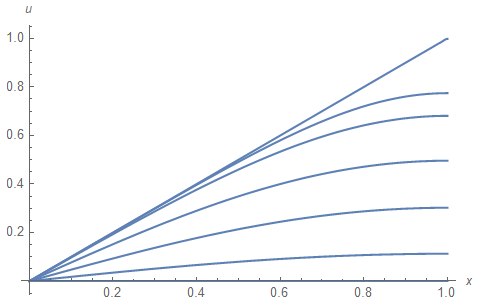
\includegraphics[scale=0.7]{pset2_2.png}
		\end{figure}
		
		\noindent The solution has good sense, first because the steady-state solution is zero - as suggested by the BCs and IC. Second, at $t=0$, $u(x,0) = x$. Third, the boundary condition requires the temperature at $x=0$ stay fixed and the temperature gradient at $x=1$ to be zero, which the plots also illustrate nicely. 
	\end{sln*}
	
\end{exer*}
\newpage









\begin{exer*}\textbf{Problem 2, Lesson 7}
	What are the eigenvalues and eigenfunctions of the Sturm-Liouville problem?
	\begin{align*}
	&ODE: X'' + \lambda X = 0,\,\,\,\,\,\,\,\,\,\,\, 0<x<1\\
	&BCs:  
	\begin{cases}
	X(0) = 0\\
	X'(1) = 0
	\end{cases}
	\end{align*}
	What are the functions $p(x)$, $q(x)$, and $r(x)$ in the general Sturm-Liouville problem for this equation? 
	
	\begin{sln*} 
		$\,$
		\begin{enumerate}
			\item $p(x) = 1$.
			\item $q(x) = 0$.
			\item $r(x) = 1$.
		\end{enumerate}
		To find the eigenvalues and the eigenfunctions, we have to solve the IVP. By the ODE, we know that 
		\begin{align*}
		X(x) = A\sin(\sqrt{\lambda}x) + B\cos(\sqrt{\lambda} x).
		\end{align*}
		Applying the initial conditions, we find 
		\begin{align*}
		B = 0\\
		-A\sqrt{\lambda}\cos(\sqrt{\lambda}) = 0.
		\end{align*}
		i.e., for $n$ odd, we find the eigenvalues:
		\begin{align*}
		\lambda_n = \left( \frac{n\pi}{2} \right)^2.
		\end{align*}
		And so the eigenfunctions are
		\begin{align*}
		X_n(x) = A_n\sin\left( \frac{n\pi x}{2} \right).
		\end{align*}
	\end{sln*}
\end{exer*}
\newpage









\begin{exer*}\textbf{2. }\textbf{Problem 3, Lesson 7}
	Solve the following problem with insulated boundaries:
	\begin{align*}
	&PDE: u_t = u_{xx},\,\,\,\,\,\,\,\,\,\,\, 0<x<1, 0<t<\infty\\
	&BCs:  
	\begin{cases}
	u_x(0,t) = 0\\
	u_x(1,t) = 0
	\end{cases} 0 < t < \infty\\
	&IC: u(x,0) = x,\,\,\,\,\,\,\,\,\,\,\, 0 \leq x\leq 1
	\end{align*}
	Does your solution agree with your interpretation of the problem? What is the steady-state solution? Does this make sense? 
	\begin{sln*}
		$\,$\\
		
		Let $u(x,t) = U(x,t) + S(x,t)$ where $S(x,t)$ is the steady-state and $U(x,t)$ is the transient solution. We can construct the steady-state solution as
		\begin{align*}
		S(x,t) = A(t)\left(1 -x \right) + B(t)x.
		\end{align*}
		As before, by applying the boundary conditions, we require that $A(t)$ and $B(t)$ solve the following linear system
		\begin{align*}
		\begin{pmatrix}
		-1 & 1\\
		-1 & 1
		\end{pmatrix}
		\begin{pmatrix}
		A(t) \\ B(t)
		\end{pmatrix}
		=
		\begin{pmatrix}
		0\\0
		\end{pmatrix}.
		\end{align*}
		The system has infinitely many solutions, but we get $A(t) = B(t)$. Assuming that at steady-state, $u_t = u_{xx} = 0 = S_t$, we get
		\begin{align*}
		S(x,t) = A(t)(1-x) + A(t)x = A(t) = \Lambda
		\end{align*}
		where $\Lambda$ is constant.\\
		
		\noindent Applying separation of variables to this PDE, we know that 
		\begin{align*}
		T(t) = e^{-\lambda^2 t}\\
		X_n(x) = A\cos(\lambda x)  + B\sin(\lambda x).
		\end{align*}
		Applying the boundary conditions, 
		\begin{align*}
		B&= 0\\
		\lambda_n &= n\pi.
		\end{align*}
		So, the general solution is
		\begin{align*}
		u(x,t) = \Lambda + \sum_{n=1}^\infty A_n e^{-(n\pi)^2 t}\cos(n\pi x).
		\end{align*}
		Next, we want to find the coefficients $A_n$. Since there is a $\cos$ involved, we will use Fourier's trick with a cosine and the identity
		\begin{align*}
		\int_{0}^1\cos(m\pi x)\cos(n\pi x) = \frac{1}{2}\delta^m_n.
		\end{align*}
		This gives
		\begin{align*}
		\int_{0}^1 u_0(x)\cos(m\pi x)\,dx &= \int_{0}^1 \cos(m\pi x)\sum_{n=1}^\infty A_n \cos(n\pi x)\,dx\\
		&= \sum_{n=1}^\infty A_n \frac{1}{2}\delta^n_m\\
		&= \frac{A_m}{2}.
		\end{align*}
		So, we can compute $A_m$ in Mathematica (or by integration by parts):
		\begin{align*}
		A_m = 2\int_{0}^1 x\cos(m\pi x)\,dx &= \frac{2 (\pi  m \sin (\pi  m)+\cos (\pi  m)-1)}{\pi ^2 m^2}\\
		&= \frac{2(\cos(\pi m - 1))}{m^2\pi^2}\\
		&= \begin{cases}
		\frac{-4}{m^2\pi^2},\,\,\,\,\,\, m \text{ odd}\\
		0,\,\,\,\,\,\,\,\, m \text{ even}.
		\end{cases}
		\end{align*}
		The general solution is then
		\begin{align*}
		u(x,t) &= \Lambda-\frac{4}{\pi^2}\sum_{n=1}^\infty \frac{1}{n^2}e^{-(n\pi)^2 t}\cos(n\pi x),\,\,\, n \text{ odd}\\
		&= \Lambda-\frac{4}{\pi ^2}e^{-(\pi)^2 t}\cos(\pi x)    -\frac{4}{9 \pi ^2}e^{-(3\pi)^2 t}\cos(3\pi x)        -\frac{4}{25 \pi ^2}e^{-(5\pi)^2 t}\cos(5\pi x) + \dots
		\end{align*}
		To find the steady-state solution, we only need to look for $\Lambda$ such that $u(0,0) = 0$ (to satisfy the initial condition), i.e.,
		\begin{align*}
		\Lambda &= \frac{4}{\pi^2}\sum^\infty_{n=1}\frac{1}{n^2},\,\,\, n \text{ odd}\\
		&= \frac{1}{2}.
		\end{align*}
		
		So steady-state solution is $S(x,t) = 1/2$, and the full solution is
		\begin{align*}
		u(x,t) &= \frac{1}{2}-\frac{4}{\pi^2}\sum_{n=1}^\infty \frac{1}{n^2}e^{-(n\pi)^2 t}\cos(n\pi x),\,\,\, n \text{ odd}\\
		&= \frac{1}{2}-\frac{4}{\pi ^2}e^{-(\pi)^2 t}\cos(\pi x)    -\frac{4}{9 \pi ^2}e^{-(3\pi)^2 t}\cos(3\pi x)        -\frac{4}{25 \pi ^2}e^{-(5\pi)^2 t}\cos(5\pi x) + \dots
		\end{align*}
		
		\noindent Mathematica code:
		\begin{lstlisting}
		Simplify[Integrate[Cos[m*Pi*x]*Cos[n*Pi*x], {x, 0, 1}]]
		(m Cos[n \[Pi]] Sin[m \[Pi]] - n Cos[m \[Pi]] Sin[n \[Pi]])/(
		m^2 \[Pi] - n^2 \[Pi])
		
		2*Integrate[x*Cos[m*Pi*x], {x, 0, 1}]
		(2 (-1 + Cos[m \[Pi]] + m \[Pi] Sin[m \[Pi]]))/(m^2 \[Pi]^2)
		
		A[m_] := (2 (-1 + Cos[m \[Pi]] + m \[Pi] Sin[m \[Pi]]))/(m^2 \[Pi]^2)
		Table[A[m], {m, 1, 7}]
		{-(4/\[Pi]^2), 0, -(4/(9 \[Pi]^2)), 0, -(4/(25 \[Pi]^2)), 0, -(4/(
		49 \[Pi]^2))}
		
		N[Sum[(4/Pi^2)*(1/(2 n - 1)^2)*1, {n, 1, 10000}]]
		0.49999
		\end{lstlisting}
	\end{sln*}
\end{exer*}


\newpage
\subsection{Problem set 3} 

\begin{exer*}\textbf{1.}
	For the following equations and associated boundary conditions (together, Sturm-Liouville Problems),
	determine the form of the eigenfunctions and give a formula (in terms of the determinant as we did in lecture) of
	the associated eigenvalues $\lambda$. Find an approximate value for $\lambda_1$, the smallest eigenvalue and estimate $\lambda_n$ for large
	values of $n$.\\
	
	Recall from class that $\lambda$ was an eigenvalue of the associated Sturm-Liouville Problem:
	\begin{align*}
	\begin{cases}
	\text{ODE: }\hspace{0.5cm} L[u](x) = \lambda r(x)u(x)\hspace{0.5cm} 0<x<1\\
	\text{BC1: }\hspace{0.5cm} a_1u(0) + b_1 u'(0) = 0\\
	\text{BC2: }\hspace{0.5cm} a_2u(1) + b_2u'(1) = 0
	\end{cases}
	\end{align*}
	where $L[u] = -(p(x)u'(x))' + q(x)u(x)$ provided, for linearly independent solutions $u_1$ and $u_2$ to the differential
	equation $L[u] = \lambda ru$,
	\begin{align*}
	\det(A(\lambda)) = \det\begin{pmatrix}
	a_1u_1(0) + b_1 u'_1(0) & a_1u_2(0) + b_1 u'_2(0)\\
	a_2u_1(1) + b_2 u'_1(1) & a_2u_2(1) + b_2 u'_2(1)
	\end{pmatrix} = 0.
	\end{align*}
	
	\noindent\rule{\textwidth}{0.5pt}
	\begin{enumerate}
		\item $y'' - \lambda y = 0\hspace{0.5cm} y(0) + y'(0) = 0, y(1) = 0.$\\
		
		\begin{sln*}
			First, we identity:
			\begin{align*}
			&p(x) = 1,\hspace{0.5cm} q(x) = 0,\hspace{0.5cm} r(x) = -1.\\
			&a_1 = 1\hspace{0.5cm} b_1 = 1,\hspace{0.5cm}a_2 = 1,\hspace{0.5cm} b_2 = 0.
			\end{align*}
			
			The associated S-L problem is
			\begin{align*}
			\begin{cases}
			\text{ODE: }\hspace{0.5cm} L[y](x) = y'' = -\lambda y\hspace{0.5cm} 0<x<1\\
			\text{BC1: }\hspace{0.5cm} y(0) + y'(0) = 0\\
			\text{BC2: }\hspace{0.5cm} y(1) = 0
			\end{cases}
			\end{align*}
			The general solution to the ODE has the form
			\begin{align*}
			y(x) = \begin{pmatrix}
			y_1 & y_2
			\end{pmatrix}\begin{pmatrix}
			C_1\\C_2
			\end{pmatrix}= 
			\begin{pmatrix}
			e^{i\sqrt{\lambda}x}&e^{-i\sqrt{\lambda} x}
			\end{pmatrix}
			\begin{pmatrix}
			C_1\\C_2
			\end{pmatrix}
			\end{align*}
			where $C_1$ and $C_2$ are determined by the BCs, which give rise to the system 
			\begin{align*}
			\begin{pmatrix}
			0\\0
			\end{pmatrix} = A\begin{pmatrix}
			C_1\\C_2
			\end{pmatrix} = \begin{pmatrix}
			1 + i\sqrt{\lambda} &  1 -i\sqrt{\lambda}  \\  e^{i\sqrt{\lambda}}  & e^{-i\sqrt{\lambda}} 
			\end{pmatrix}
			\begin{pmatrix}
			C_1\\C_2
			\end{pmatrix}
			\end{align*}	
			To get non-trivial solutions, we require $\det(A(\lambda)) = 0$, i.e., 
			\begin{align*}
			(1+i\sqrt{\lambda})e^{-i\sqrt{\lambda}} - (1-i\sqrt{\lambda})e^{i\sqrt{\lambda}} = 0. 
			\end{align*}
			Let $\lag = \sqrt{\lambda}^2$, (we're assuming $\lambda$ is positive in this problem)
			\begin{align*}
			0 &= (1+i\lag)e^{-i\lag} - (1-i\lag)e^{i\lag}\\
			&= (1+i\lag)(\cos\lag - i\sin\lag) - (1-i\lag)(\cos\lag + i\sin\lag)\\
			&= 2i (\lag\cos\lag - \sin\lag)
			\end{align*}
			if and only if
			\begin{align*}
			\boxed{\tan\lag = \lag}.
			\end{align*}
			Since we require $\lambda\neq 0$ is get non-trivial solutions, we only consider $\lag_1,\lag_2,\dots$. Numerically approximate in Mathematica gives
			\begin{align*}
			&\lag_1 \approx 4.493409457909114\\
			&\lag_n \approx n.
			\end{align*}
			Converting $\lag$ back to $\lambda$ and requiring $\lambda < 0$, we get
			\begin{empheq}[box=\fbox]{align} 
			&\lambda_1 \approx 20.1907\nonumber\\
			&\lambda_n \approx n^2\hspace{0.5cm} n \text{ large}\nonumber 
			\end{empheq}
			While we can't find $C_1$ and $C_2$ exactly, we can find their ratio from the linear system:
			\begin{align*}
			\frac{C_1}{C_2} = \frac{-e^{-i\sqrt{\lambda}}}{e^{i\sqrt{\lambda}}} = -e^{-2i\sqrt{\lambda}}.
			\end{align*}
			
			The unnormalized eigenfunction thus has the form 
			\begin{align*}
			y(x) = -e^{-2i\sqrt{\lambda_n}}e^{i\sqrt{\lambda_n}x} + e^{-i\sqrt{\lambda_n}x} = -e^{i\sqrt{\lambda_n}(x-2)} + e^{-i\sqrt{\lambda_n}x} .
			\end{align*}	
			Since $r(x) = -1$, normalizing $y$ only involves the modulus square of it:
			\begin{align*}
			\vert\vert y \vert\vert^2 &= -(-e^{i\sqrt{\lambda_n}(x-2)} + e^{-i\sqrt{\lambda_n}x})(-e^{-i\sqrt{\lambda_n}(x-2)} + e^{i\sqrt{\lambda_n}x})\\
			&= -2 + e^{i\sqrt{\lambda_n}(x-2) + i\sqrt{\lambda_n}x} + e^{-i\sqrt{\lambda_n}x  -i\sqrt{\lambda_n}(x-2) }\\
			&= -2 + e^{i\sqrt{\lambda_n}(x-2)} + e^{-i\sqrt{\lambda_n}(x-2)}\\
			&= -2 + \cos\left(\sqrt{\lambda_n} (x-2)\right).
			\end{align*}
			The normalizing condition requires 
			\begin{align*}
			1 = -\int^1_0 2 - \cos\left(\sqrt{\lambda_n} (x-2)\right)\,dx.
			\end{align*}
			Integrating in Mathematica and normalizing gives the form for an eigenfunction:
			\begin{align*}
			\boxed{y_n(x,\lambda_n) =  \frac{\sqrt{\lambda_n}}{\sin\sqrt{\lambda_n} (1- 2 \cos\sqrt{\lambda_n})+2\sqrt{\lambda_n}}\left( e^{i\sqrt{\lambda_n}(x-2)} - e^{-i\sqrt{\lambda_n}x}  \right)}
			\end{align*}
		\end{sln*}
		
		Mathematica code:
		\begin{lstlisting}
		Simplify[(1 + I*L) (Cos[L] - I*Sin[L]) - (1 - I*L) (Cos[L] + 
		I*Sin[L])]
		2 I (L Cos[L] - Sin[L])
		
		t[L_] := Tan[L] - L; val = 0.000000000001; 
		FindRoot[val == t[L], {L, 4}]
		{L -> 4.49341}
		Show[Plot[Tan[L], {L, 0, 10}], Plot[L, {L, 0, 10}]]
		
		Simplify[Integrate[2 - Cos[A*(x - 2)], {x, 0, 1}]]
		2 + ((1 - 2 Cos[A]) Sin[A])/A
		\end{lstlisting}
		
		\begin{figure}[h!]
			\centering
			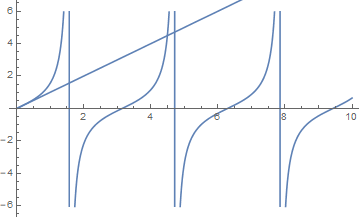
\includegraphics[scale=0.7]{pde_3_1.png}
		\end{figure}
		
		\newpage
		
		
		\item $y'' + \lambda y = 0\hspace{0.5cm} y'(0) = 0, y(1) + y'(1) = 0. $\\
		\noindent\rule{\textwidth}{0.5pt}
		\begin{sln*}
			First, we identity:
			\begin{align*}
			&p(x) = 1,\hspace{0.5cm} q(x) = 0,\hspace{0.5cm} r(x) = 1.\\
			&a_1 = 0\hspace{0.5cm} b_1 = 1,\hspace{0.5cm}a_2 = 1,\hspace{0.5cm} b_2 = 1.
			\end{align*}
			
			The associated S-L problem is
			\begin{align*}
			\begin{cases}
			\text{ODE: }\hspace{0.5cm} L[y](x) = y'' = -\lambda y\hspace{0.5cm} 0<x<1\\
			\text{BC1: }\hspace{0.5cm} y'(0) = 0\\
			\text{BC2: }\hspace{0.5cm} y(1) + y'(1) = 0
			\end{cases}
			\end{align*}
			The general solution to the ODE has the form
			\begin{align*}
			y(x) = \begin{pmatrix}
			y_1 & y_2
			\end{pmatrix}
			\begin{pmatrix}
			C_1\\C_2
			\end{pmatrix} = 
			\begin{pmatrix}
			\cos\sqrt{\lambda} x & \sin\sqrt{\lambda} x
			\end{pmatrix}
			\begin{pmatrix}
			C_1\\C_2
			\end{pmatrix}
			\end{align*}
			where $C_1$ and $C_2$ are determined by the BCs, which give rise to the system
			\begin{align*}
			\begin{pmatrix}
			0\\0
			\end{pmatrix} = A\begin{pmatrix}
			C_1\\C_2
			\end{pmatrix} = \begin{pmatrix}
			-\sqrt{\lambda} &  \sqrt{\lambda}  \\  \cos\sqrt{\lambda} - \sqrt{\lambda}\sin\sqrt{\lambda}  & \sin\sqrt{\lambda} + \sqrt{\lambda}\cos\sqrt{\lambda}
			\end{pmatrix}
			\begin{pmatrix}
			C_1\\C_2
			\end{pmatrix}
			\end{align*}
			To get non-trivial solutions, we require $\det(A) = 0$, i.e., 
			\begin{align*}
			0 &= -\sqrt{\lambda}(\sin\sqrt{\lambda} + \sqrt{\lambda}\cos\sqrt{\lambda} ) - \sqrt{\lambda}(\cos\sqrt{\lambda} - \sqrt{\lambda}\sin\sqrt{\lambda})\\
			0 &=  \sin\sqrt{\lambda} + \sqrt{\lambda}\cos\sqrt{\lambda} + \cos\sqrt{\lambda} - \sqrt{\lambda}\sin\sqrt{\lambda}\\
			0 &= (1-\sqrt{\lambda})\sin\sqrt{\lambda} + (1+\sqrt{\lambda})\cos\sqrt{\lambda}.
			\end{align*}
			This means
			\begin{align*}
			\boxed{\tan\sqrt{\lambda} = \frac{\sqrt{\lambda} + 1}{\sqrt{\lambda} - 1}}
			\end{align*}
			Numerically approximate in Mathematica gives
			\begin{empheq}[box=\fbox]{align} 
			&\lambda_1 \approx 1.97184\nonumber\\
			&\lambda_n \approx n \hspace{0.5cm} n \text{ large}\nonumber 
			\end{empheq}
			While we can't find $C_1$ and $C_2$ exactly, we can find their ratio from the linear system:
			\begin{align*}
			\frac{C_1}{C_2} = \frac{-\sqrt{\lambda}}{-\sqrt{\lambda}} = 1.
			\end{align*}
			The unnormalized eigenfunction thus has the form
			\begin{align*}
			y_n(x,\lambda_n) = \cos\sqrt{\lambda_n} x + \sin\sqrt{\lambda_n} x.
			\end{align*}
			The normalizing condition requires
			\begin{align*}
			1 = \int^1_0 \cos\sqrt{\lambda_n} x + \sin\sqrt{\lambda_n}  x\,dx.
			\end{align*}
			Integrating and normalizing gives the form for an eigenfunction:
			\begin{align*}
			\boxed{ \frac{\sqrt{\lambda_n}}{1 - \cos\sqrt{\lambda_n} + \sin\sqrt{\lambda_n}}\left( \cos\sqrt{\lambda_n} x + \sin\sqrt{\lambda_n} x \right) }
			\end{align*}
			
			Mathematica code:
			\begin{lstlisting}
			tan[L_] := Tan[Sqrt[L]] - (Sqrt[L] + 1)/(Sqrt[L] - 1); 
			inv = 0.000000001; FindRoot[
			tan[L] == inv, {L, 2}]
			{L -> 1.97184}
			
			Show[Plot[Tan[Sqrt[L]], {L, 0, 10}], 
			Plot[(Sqrt[L] + 1)/(Sqrt[L] - 1), {L, 0, 10}]]
			
			Integrate[Cos[L*x] + Sin[L*x], {x, 0, 1}]
			(1 - Cos[L] + Sin[L])/L
			\end{lstlisting}
			\begin{figure}[h!]
				\centering
				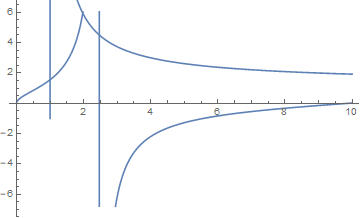
\includegraphics[scale=0.7]{pde_3_2.png}
			\end{figure}
		\end{sln*}
		
		
		
		
		
		\newpage
	\end{enumerate}
	
\end{exer*}

\newpage 

\begin{exer*}\textbf{2. } In lecture, we saw that the linear operator $$L[u] = -(p(x)u'(x))' + q(x)u(x)$$ had the property that
	\begin{align*}
	\int^1_0 (vL[u] - uL[v])\,dx = 0
	\end{align*}
	whenever $u$ and $v$ are twice-continuously differentiable functions which satisfy the boundary conditions of the Strum-Liouville Problem. \\
	
	In class, we assumed $b_1$ and $b_2$ were non-zero. Here, show that the result remains valid
	provided $b_1$ or $b_2$ is zero. Do $u$ and $v$ have to be eigenfunctions of the S-L problem for the property above to hold? Or, is it simply required that $u$ and $v$ satisfied the boundary conditions? Assume the identity:
	\begin{align*}
	\int^1_0 (fL[g] - gL[f])\,dx = p(x)(g'(x)f(x) - f'(x)g(x))\bigg\vert^1_0
	\end{align*}
	which is true for all twice-continuously differentiable functions on the interval $[0,1]$.
	
	\noindent\rule{\textwidth}{0.5pt}
	
	\begin{sln*}
		Assume that
		\begin{align*}
		\int^1_0 (fL[g] - gL[f])\,dx = p(x)(g'(x)f(x) - f'(x)g(x))\bigg\vert^1_0,
		\end{align*}
		and (without loss of generality) $b_1 = 0, b_2\neq 0$, i.e., $a_1\phi(0) = 0$ and $a_2\phi(1) + b_2\phi'(1) =0 $ for $\phi = v$ or $u$. If this implies $\phi(1) = \phi(0) = 0$, then  we have
		\begin{align*}
		\int^1_0 (vL[u] - uL[v])\,dx &= p(x)(u'(x)v(x) - v'(x)u(x))\bigg\vert^1_0\\
		&= p(1)(u'(1)v(1) - v'(1)u(1)) - p(0)(u'(0)v(0) - v'(0)u(0))\\
		&= p(1)(u'(1)v(1) - v'(1)u(1))\\
		&= p(1)\left( \frac{-b_2u(1)}{a_2}v(1) - \frac{-b_2v(1)}{a_2}u(1) \right)\\
		&= 0.
		\end{align*}
		If $a_1, a_2 = 0$ then there are no boundary conditions, so we reject this possibility.\\
		
		Observe that the identity holds regardless of whether $u$ and $v$ are eigenfunctions of the S-L problem. It is simply required that $u$ and $v$ satisfied the boundary conditions. 
	\end{sln*}
\end{exer*}


\newpage


\begin{exer*}\textbf{3. }
	Consider a second-order linear differential operator
	\begin{align*}
	M[u](x) = \kappa_2 u''(x) + \kappa_1(x)u'(x) + \kappa_0 u(x)
	\end{align*}
	and linear homogeneous boundary conditions 
	\begin{align*}
	\begin{cases}
	\text{BC1: }\hspace{0.5cm} a_1u(0) + b_1u'(0) = 0\\
	\text{BC2: }\hspace{0.5cm} a_2u(1) + b_2 u'(1) = 0
	\end{cases}
	\end{align*}
	where $(a_1,b_1) \neq (0,0)$ and $(a_2,b_2) \neq (0,0)$; we take both the operator $M$ and the BCs to be defined for all twice-continuously differentiable functions $u$ on $[0,1]$. We say that the operator $M[u]$, when restricted to the BCs is \textit{formally self-adjoint} provided
	\begin{align*}
	\int^1_0 uL[v] - vL[u]\,dx = 0
	\end{align*}
	whenever $u$ and $v$ satisfy the BCs. \\
	
	Are the following operators restricted to the given boundary conditions formally self-adjoint? Justify your
	answer.
	
	
	\noindent\rule{\textwidth}{0.5pt}
	
	\begin{enumerate}
		\item $M[u] = u''+ u' + 2u,\hspace{0.5cm} u(0) = u(1) = 0.$\\
		
		\begin{sln*}
			$M[u]$ is self-adjoint if
			\begin{align*}
			\int^1_0 (vM[u] - uM[v])\,dx = 0.
			\end{align*}
			We first expand and simplify the integrand.
			\begin{align*}
			vM[u] - uM[v] &= v( u''+ u' + 2u) - u( v''+ v' + 2v)\\
			&= (vu'' - uv'') + (vu' - uv').
			\end{align*}
			Integrating both sides gives
			\begin{align*}
			\int^1_0 (vM[u] - uM[v])\,dx &= \int^1_0 (vu'' - uv'')\,dx + \int^1_0 (vu' - uv')\,dx.
			\end{align*} 
			Consider the first term.
			\begin{align*}
			\int^1_0 (vu'' - uv'')\,dx &= \int^1_0 vu''\,dx - \int^1_0 uv''\,dx\\
			&= vu'\bigg\vert^1_0 - \int^1_0 v'u'\,dx - uv'\bigg\vert^1_0 +  \int^1_0 u'v'\,dx\\
			&= vu' - uv' \bigg\vert^1_0\\
			&= (v(1)u'(1) - u(1)v'(1)) - (v(0)u'(0) - u(0)v'(0))\\
			&= 0. 
			\end{align*}
			We can attempt to simplify the second term, in a similar fashion:
			\begin{align*}
			\int^1_0 (vu' - uv')\,dx &= \int^1_0 vu'\,dx - \int^1_0   uv'\,dx\\
			&= vu\bigg\vert^1_0 - \int^1_0   uv'\,dx - \int^1_0   uv'\,dx\\
			&= v(1)u(1) - v(0)u(0) - \int^1_0   uv'\,dx - \int^1_0   uv'\,dx\\
			&= -2\int^1_0   uv'\,dx\\
			&\neq 0.
			\end{align*} 
			Therefore $M[u]$ is not self-adjoint. 
		\end{sln*}
		\newpage
		
		
		
		
		
		
		\item $M[u] = (1+x^2)u'' + 2xu' + u,\hspace{0.5cm} u'(0) = u(1) + 2u'(1) = 0.$\\
		\noindent\rule{\textwidth}{0.5pt}
		\begin{sln*}
			$M[u]$ is self-adjoint if
			\begin{align*}
			\int^1_0 (vM[u] - uM[v])\,dx = 0.
			\end{align*}
			We first expand and simplify the integrand.
			\begin{align*}
			vM[u] - uM[v] &= v((1+x^2)u'' + 2xu' + u) - u((1+x^2)v'' + 2xv' + v)\\
			&= (1+x^2)(vu'' - uv'') + 2x(vu' - uv').
			\end{align*} 
			Integrating both sides gives
			\begin{align*}
			\int^1_0 (vM[u] - uM[v])\,dx &= \int^1_0 (1+x^2)(vu'' - uv'')\,dx + \int^1_0 2x(vu' - uv')\,dx.\\
			&=\int^1_0 vu'' - uv''\,dx + \int^1_0 x^2(vu'' - uv'')\,dx\\
			&\hspace{0.5cm} + \int^1_0 2x(vu' - uv')\,dx.
			\end{align*}
			Consider the first term:
			\begin{align*}
			\int^1_0 (vu'' - uv'')\,dx &= \int^1_0 (vu'' - uv'')\,dx\\
			&= vu'\bigg\vert^1_0 - uv'\bigg\vert^1_0\\
			&= v(1)u'(1) - v(0)u'(0) - u(1)v'(1) + u(0)v'(0)\\
			&= v(1)u'(1) - u(1)v'(1)\\
			&= +2v'(1)\frac{1}{2}u(1) - u(1)v'(1)\\
			&= 0.
			\end{align*}
			Consider the second term:
			\begin{align*}
			\int^1_0 x^2(vu'' - uv'')\,dx &= \int^1_0 x^2 \left[ (vu')' - u'v' - (uv')' + u'v'  \right]\,dx\\
			&= \int^1_0 x^2\left[ (vu')' - (uv')' \right]\,dx\\
			&= x^2(vu')\bigg\vert^1_0 - \int^1_0 2x(vu')\,dx - x^2(uv')\bigg\vert^1_0 + \int^1_0 2x(uv')\,dx\\
			&= v(1)u'(1) - u(1)v'(1) - \int^1_0 2x(vu' - uv')\,dx\\
			&= +2v'(1)\frac{1}{2}u(1) - u(1)v'(1) - \int^1_0 2x(vu' - uv')\,dx.
			\end{align*} 
			Putting everything together, we find a cancellation:
			\begin{align*}
			\int^1_0 (vM[u] - uM[v])\,dx &= - \int^1_0 2x(vu' - uv')\,dx + \int^1_0 2x(vu' - uv')\,dx\\
			&= 0.
			\end{align*} 
			Therefore, $M[u]$ is self-adjoint. 
			
			
			
			
		\end{sln*}
		
		
		
		
		
		
		\newpage
		\item $M[u] = (1+x^2)u'' + 2xu' + u,\hspace{0.5cm} u(0) - u'(1) = u'(0) + 2u(1) = 0.$\\
		\noindent\rule{\textwidth}{0.5pt}
		\begin{sln*}
			$M[u]$ is self-adjoint if 
			\begin{align*}
			\int^1_0 (vM[u] - uM[v])\,dx = 0.
			\end{align*}
			We first expand and simplify the integrand
			\begin{align*}
			vM[u] - uM[v] &= v((1+x^2)u'' + 2xu' + u) - u((1+x^2)v'' + 2xv' + v)\\
			&= (1+x^2)(vu'' - uv'') + 2x(vu' - uv').
			\end{align*}
			Integrating both sides gives
			\begin{align*}
			\int^1_0 (vM[u] - uM[v])\,dx &= \int^1_0 (1+x^2)(vu'' - uv'')\,dx + \int^1_0 2x(vu' - uv')\,dx.\\
			&=\int^1_0 vu'' - uv''\,dx + \int^1_0 x^2(vu'' - uv'')\,dx\\
			&\hspace{0.5cm} + \int^1_0 2x(vu' - uv')\,dx.
			\end{align*}
			Consider the first term:
			\begin{align*}
			\int^1_0 (vu'' - uv'')\,dx &= \int^1_0 (vu'' - uv'')\,dx\\
			&= vu'\bigg\vert^1_0 - uv'\bigg\vert^1_0\\
			&= v(1)u'(1) - v(0)u'(0) - u(1)v'(1) + u(0)v'(0).
			\end{align*}
			Consider the second term:
			\begin{align*}
			\int^1_0 x^2(vu'' - uv'')\,dx &= \int^1_0 x^2 \left[ (vu')' - u'v' - (uv')' + u'v'  \right]\,dx\\
			&= \int^1_0 x^2\left[ (vu')' - (uv')' \right]\,dx\\
			&= x^2(vu')\bigg\vert^1_0 - \int^1_0 2x(vu')\,dx - x^2(uv')\bigg\vert^1_0 + \int^1_0 2x(uv')\,dx\\
			&= v(1)u'(1) - u(1)v'(1) - 2x\int^1_0 (vu' - uv')\,dx.
			\end{align*}
			Putting everything together, we find a cancellation:
			\begin{align*}
			\int^1_0 (vM[u] - uM[v])\,dx &= -\int^1_0 2x(vu' - uv')\,dx + \int^1_0 2x(vu' - uv')\,dx\\&\hspace{0.5cm} + 2v(1)u'(1) - v(0)u'(0) - 2u(1)v'(1) + u(0)v'(0)  \\
			&= 2v(1)u'(1) - v(0)u'(0) - 2u(1)v'(1) + u(0)v'(0)\\
			&= -v'(0)u(0) - v(0)u'(0) + u'(0)v(0) + u(0)v'(0)\\
			&= 0.
			\end{align*} 
			Therefore, $M[u]$ is self-adjoint. 
			
			
			
		\end{sln*}
		
		
		
	\end{enumerate}
	
	
\end{exer*}



\newpage

\begin{exer*}\textbf{4. Problem 3, Lesson 8} 
	$\,$\\
	Solve
	\begin{align*}
	&\text{PDE: }\hspace{0.5cm} u_t = u_{xx} - u\hspace{0.5cm} 0<x<1, 0 < t < \infty\\
	&\text{BCs: }\hspace{0.5cm} \begin{cases}
	u(0,t) = 0\\
	u(1,t) = 0
	\end{cases}\hspace{0.5cm} 0 < t < \infty\\
	&\text{IC: } u(x,0) = \sin(\pi x) \hspace{0.5cm} 0 \leq x \leq 1.
	\end{align*}
	directly by separation of variables without making any preliminary transformation. Does your solution agree with the solution you would obtain if
	the transformation
	\begin{align*}
	u(x,t) = e^{-t}w(x,t)
	\end{align*}
	were made in advance?
	
	\noindent\rule{\textwidth}{0.5pt}
	\begin{sln*}
		Let
		\begin{align*}
		u(x,t) = X(x)T(t).
		\end{align*}
		The PDE tells us that
		\begin{align*}
		T_t X = X_{xx} T - XT.
		\end{align*}
		Applying the BCs, we get
		\begin{align*}
		\begin{cases}
		T_t(t)X(0) = X_{xx}(0)T(t)\\
		T_t(t)X(1) = X_{xx}(1)T(t),
		\end{cases}
		\end{align*}
		i.e.,
		\begin{align*}
		\frac{T_t(t)}{T(t)} = \frac{X_{xx}}{X} = -\lambda^2,
		\end{align*}
		where $\mu$ is a constant. So,
		\begin{align*}
		\begin{cases}
		T(t) = e^{-\lambda^2 t}\\
		X(x) = A\cos\lambda x + B\sin\lambda x
		\end{cases}
		\end{align*}
		Applying the BCs, we get
		\begin{align*}
		A &= 0\\
		\lambda &= n\pi, \hspace{0.5cm} n = 0,1,2,3,\dots
		\end{align*}
		So the general solution (to the homogeneous case)is
		\begin{align*}
		u(x,t) = \sum_{n=0}^\infty e^{-(n\pi)^2 t}B_n \sin(n\pi x),
		\end{align*}
		where $B_n$ can be solved by applying the IC:
		\begin{align*}
		\int^1_0 \sin(\pi x)\sin(m\pi x)\,dx &= \int^1_0 \sum_{n=0}^\infty B_n \sin(n\pi x)\sin(m\pi x)\,dx\\
		&= \frac{1}{2}B_n \delta^n_m\\
		&= \frac{1}{2}B_m.
		\end{align*}
		This gives
		\begin{align*}
		B_n = 2\int^1_0 \sin(\pi x)\sin(n\pi x)\,dx = \delta^1_n.
		\end{align*}
		So the solution to the homogeneous PDE is
		\begin{align*}
		u(x,t) = e^{-\pi^2 t}\sin(\pi x).
		\end{align*}
		Since we have essentially been treating this IBVP as one with a homogeneous PDE, we should check whether our general solution satisfies the PDE:
		\begin{align*}
		u_t &= u_{xx} - u\\
		-\pi^2 u &\neq -(\pi^2 + 1)u.
		\end{align*} 
		We see that the solution to the homogeneous case does not quite work yet. However, we notice that multiplying the existing solution by $e^{-t}$ can ``fix'' this problem without changing the spatial part of the solution. So, the working solution is
		\begin{align*}
		\boxed{u(x,t) = e^{-(\pi^2 +1 )t}\sin\pi x}
		\end{align*} 
		Now, if we apply the transformation $u(x,t) = e^{-t}w(x,t)$ in advance, then the extra factor of $e^{-t}$ will be taken care of in advance, and the IBVP will be transformed into one with both homogeneous PDE and BCs that involves $w(x,t)$ rather than $v(x,t)$. First, we can look at how the PDE changes:
		\begin{align*}
		u_t &\to -e^{-t}w(x,t) + e^{-t}w_t(x,t)\\
		u_{xx} - u &\to e^{-t}w_{xx}(x,t) - e^{-t}w(x,t).
		\end{align*}
		For the original PDE to hold, we require that
		\begin{align*}
		w_t = w_{xx}.
		\end{align*}
		Since the BCs and ICs are time-independent, the transformation simply allows us to replace $v$ by $w$. So, the new IBVP is
		\begin{align*}
		\begin{cases}
		&\text{PDE: }\hspace{0.5cm} w_t = w_{xx}\hspace{0.5cm} 0<x<1, 0 < t < \infty\\
		&\text{BCs: }\hspace{0.5cm} \begin{cases}
		w(0,t) = 0\\
		w(1,t) = 0
		\end{cases}\hspace{0.5cm} 0 < t < \infty\\
		&\text{IC: } w(x,0) = \sin(\pi x) \hspace{0.5cm} 0 \leq x \leq 1.
		\end{cases}
		\end{align*}
		
		This is exactly how we treated $u(x,t)$ before correcting it to make it solve the PDE. So, our solution agrees with the solution we would obtain if the transformation $u(x,t) = e^{-t}w(x,t)$ were made in advance.
		
	\end{sln*}
	
\end{exer*}


\newpage
\subsection{Problem set 4}

\begin{exer*}\textbf{1. Problem 1, Lesson 9, Farlow}
	\begin{align*}
	u(x,t) = e^{-(\pi\alpha)^2t}\sin(\pi x) + \frac{1}{(3\pi \alpha)^2}\left[1 - e^{-(3\pi \alpha)^2 t}\right]\sin(3\pi x).
	\end{align*}
	\begin{sln*}
		We can plot $u(x,t)$ for a few time points:
		\begin{lstlisting}
U[t_, x_] := 
E^(-Pi^2 t)*Sin[Pi*x] + 
1/(3*Pi)^2*(1 - E^(-(3 Pi)^2 t))*Sin[3 Pi*t];

Show[Plot[U[0, x], {x, 0, 1}], Plot[U[0.05, x], {x, 0, 1}],
Plot[U[0.01, x], {x, 0, 1}], Plot[U[0.08, x], {x, 0, 1}], 
AxesLabel -> {x, u}]
		\end{lstlisting}
		
		\begin{figure}[h!]
			\centering
			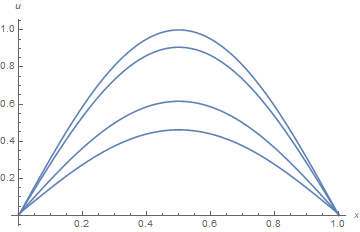
\includegraphics[scale=0.7]{pde4_1.png}
		\end{figure}
	
	The solution makes sense, because the IBVP basically describes a rod with fixed zero temperature at the ends and an initial temperature distribution of $\sin(\pi x)$ being subjected to some heat source. 
	\end{sln*}
\end{exer*}

\newpage

\begin{exer*}\textbf{2. Problem 2, Lesson 9, Farlow}\\
	Solve the IBVP:
	\begin{align*}
	&\text{PDE: } u_t = u_{xx} + \sin(\pi x) + \sin(2\pi x), \hspace{0.2cm} 0 < x < 1\hspace{0.2cm} 0 < t < \infty\\
	&\text{BCs: }\begin{cases}
	u(0,t) = 0\\
	u(1,t) = 0
	\end{cases}\hspace{0.2cm} 0 < t < \infty\\
	&\text{IC: }u(x,0) = 0\hspace{0.2cm}0\leq x\leq 1.
	\end{align*}
	
	\begin{sln*}
		We use the eigenfunction expansion method to solve this problem. The first step is finding the eigenvectors by converting the homogeneous problem:
		\begin{align*}
		&\text{PDE: } u_t = u_{xx}, \hspace{0.2cm} 0 < x < 1\hspace{0.2cm} 0 < t < \infty\\
		&\text{BCs: }\begin{cases}
		u(0,t) = 0\\
		u(1,t) = 0
		\end{cases}\hspace{0.2cm} 0 < t  \infty
		\end{align*}
		into the associated S-L problem 
		\begin{align*}
		&\text{PDE: } X_{xx} = -\lambda^2 X, \hspace{0.2cm} 0 < x < 1\hspace{0.2cm}\\
		&\text{BCs: }\begin{cases}
		X(0) = 0\\
		X(1) = 0
		\end{cases}\hspace{0.2cm},
		\end{align*}
		to which the solutions (or the eigenvectors) have the form:
		\begin{align*}
		X_n(x) = \sin(n\pi x).
		\end{align*}
		
		Next, we want to write $f(x,t) = \sin(\pi x) + \sin(2\pi x)$ in terms of the eigenvectors. Observe that we don't need Fourier Sine series here since $f(x,t)$ is already given to us as a sum of two eigenvectors:
		\begin{align*}
		f(t,x) = \sin(\pi x) + \sin(2\pi x) = \sum^\infty_{n=1}f_n(t)X_n(x) = f_1(t) \times X_1(x) + f_2(t) \times X_2(x).
		\end{align*}
		This means
		\begin{align*}
		&f_1(t) = f_2(t) = 1\\
		&f_n(t) = 0, \hspace{0.2cm}n > 2.
		\end{align*}
		Subject 
		\begin{align*}
		u(t,x) = \sum^\infty_{n=1} T_n(t)X_n(x)
		\end{align*}
		to the IBVP, where
		\begin{align*}
		f(t,x) = \sum^\infty_{n=1}f_n(t)X_n(x) = \sum^\infty_{n=1}f_n(t)\sin(n\pi x)
		\end{align*}
		gives
		\begin{align*}
		\dot{T}_n(t) + (n\pi)^2T_n(t) = f_n(t),
		\end{align*}
		to which the solution is of the form
		\begin{align*}
		T_n(t) = e^{-(n\pi)^2t}\int^t_0 f_n(s)e^{(n\pi)^2s}\,ds + T_n(0)e^{-(n\pi)^2t}.
		\end{align*}
		Since we only have non-zero $f_1(t) = f_2(t) = 1$, 
		\begin{align*}
		T_1(t) &= e^{-(\pi)^2t}\int^t_0 e^{(\pi)^2s}\,ds + T_1(0)e^{-(\pi)^2t}\\
		&= e^{-(\pi)^2t}\left(\frac{-1 + e^{\pi^2t}}{\pi^2}  + T_1(0)\right),
		\end{align*}
		and 
		\begin{align*}
		T_2(t) &= e^{-(2\pi)^2t}\int^t_0 e^{(2\pi)^2s}\,ds + T_2(0)e^{-(2\pi)^2t}\\
		&= e^{-(2\pi)^2t}\left(\frac{-1 + e^{4\pi^2t}}{4\pi^2}  + T_2(0)  \right),
		\end{align*}
		and
		\begin{align*}
		T_n(t) = T_n(0)e^{-(n\pi)^2t}, \hspace{0.2cm}n > 2.
		\end{align*}
		Next, note that because 
		\begin{align*}
		u(0,x) = u_0(x) = 0 = \sum^\infty_{n=1}T_n(0)\sin(n\pi x),
		\end{align*}
		we have
		\begin{align*}
		T_n(0) = 0,
		\end{align*}
		which means all $T_n(t) = 0$ for $n>2$ are zero. Therefore, 
		\begin{align*}
		u(t,x) &= \sum^\infty_{n=1}\left( e^{-(n\pi)^2t}\int^t_0 f_n(s)e^{(n\pi)^2s}\,ds \right)\sin(n\pi x)\\
		&= e^{-(\pi)^2t}\left(\frac{-1 + e^{\pi^2t}}{\pi^2}\right)\sin(\pi x) + e^{-(2\pi)^2t}\left(\frac{-1 + e^{4\pi^2t}}{4\pi^2} \right)\sin(2\pi x)\\
		&= \frac{1}{\pi^2}\left(1 - e^{-\pi^2 t}\right)\sin(\pi x) + \frac{1}{(2\pi)^2}e^{-(2\pi)^2t}\left(1 - e^{-(2\pi)^2t}\right)\sin(2\pi x).
		\end{align*}
		
		
	\end{sln*}
\end{exer*}

\newpage

\begin{exer*}\textbf{4. Problem 5, Lesson 9, Farlow}\\
	
	Solve the IBVP:
	\begin{align*}
	&\text{PDE: } u_t = u_{xx} + \sin(\pi x), \hspace{0.2cm} 0 < x < 1\hspace{0.2cm} 0 < t < \infty\\
	&\text{BCs: }\begin{cases}
	u(0,t) = 0\\
	u(1,t) = 0
	\end{cases}\hspace{0.2cm} 0 < t < \infty\\
	&\text{IC: }u(x,0) = 1\hspace{0.2cm}0\leq x\leq 1.
	\end{align*}
	
	\begin{sln*}
		We use the eigenfunction expansion method to solve this problem. The first step is finding the eigenvectors by converting the homogeneous problem:
		\begin{align*}
		&\text{PDE: } u_t = u_{xx}, \hspace{0.2cm} 0 < x < 1\hspace{0.2cm} 0 < t < \infty\\
		&\text{BCs: }\begin{cases}
		u(0,t) = 0\\
		u(1,t) = 0
		\end{cases}\hspace{0.2cm} 0 < t  \infty
		\end{align*}
		into the associated S-L problem 
		\begin{align*}
		&\text{PDE: } X_{xx} = -\lambda^2 X, \hspace{0.2cm} 0 < x < 1\hspace{0.2cm}\\
		&\text{BCs: }\begin{cases}
		X(0) = 0\\
		X(1) = 0
		\end{cases}\hspace{0.2cm},
		\end{align*}
		to which the solutions (or the eigenvectors) have the form:
		\begin{align*}
		X_n(x) = \sin(n\pi x).
		\end{align*}
		
		Next, we want to write $f(x,t) = \sin(\pi x)$ in terms of the eigenvectors. Observe that we don't need Fourier Sine series here since $f(x,t)$ is already given to us as a sum of two eigenvectors:
		\begin{align*}
		f(t,x) = \sin(\pi x) = \sum^\infty_{n=1}f_n(t)X_n(x) = f_1(t) \times X_1(x).
		\end{align*}
		This means
		\begin{align*}
		f_n(t) = \delta^1_n.
		\end{align*}
		Subject 
		\begin{align*}
		u(t,x) = \sum^\infty_{n=1} T_n(t)X_n(x)
		\end{align*}
		to the IBVP, where
		\begin{align*}
		f(t,x) = \sum^\infty_{n=1}f_n(t)X_n(x) = \sum^\infty_{n=1}f_n(t)\sin(n\pi x)
		\end{align*}
		gives
		\begin{align*}
		\dot{T}_n(t) + (n\pi)^2T_n(t) = f_n(t),
		\end{align*}
		to which the solution is of the form
		\begin{align*}
		T_n(t) = e^{-(n\pi)^2t}\int^t_0 f_n(s)e^{(n\pi)^2s}\,ds + T_n(0)e^{-(n\pi)^2t}.
		\end{align*}
		Since we only have non-zero $f_1(t) = 1$, 
		\begin{align*}
		T_1(t) &= e^{-(\pi)^2t}\int^t_0 e^{(\pi)^2s}\,ds + T_1(0)e^{-(\pi)^2t}\\
		&= e^{-(\pi)^2t}\left(\frac{-1 + e^{\pi^2t}}{\pi^2}  + T_1(0)\right),
		\end{align*}
		and
		\begin{align*}
		T_n(t) = T_n(0)e^{-(n\pi)^2t}, \hspace{0.2cm}n > 2.
		\end{align*}
		Next, note that because 
		\begin{align*}
		u(0,x) = u_0(x) = 1 = \sum^\infty_{n=1}T_n(0)\sin(n\pi x),
		\end{align*}
		we have
		\begin{align*}
		T_n(0) = 2\int^1_0  \sin(n \pi x)\,dx = \begin{cases}
		4/(n\pi), \hspace{0.2cm}n \text{ odd}\\
		0, \hspace{0.2cm}n \text{ even}.
		\end{cases}
		\end{align*}
		Therefore, 
		\begin{align*}
		u(t,x) &= \sum^\infty_{n=1}\left( e^{-(n\pi)^2t}\int^t_0 f_n(s)e^{(n\pi)^2s}\,ds \right)\sin(n\pi x)\\
		&= e^{-(\pi)^2t}\left(\frac{-1 + e^{\pi^2t}}{\pi^2} + \frac{4}{\pi}\right)\sin(\pi x) + \sum^\infty_{n=2}\frac{4}{n\pi}e^{-(n\pi)^2t}\sin(n\pi x),\hspace{0.2cm}n \text{ odd}\\
		&= \left(\frac{1-e^{\pi^2t}}{\pi^2} + \frac{4}{\pi}e^{-\pi^2t}\right)\sin(\pi x) + \sum^\infty_{j=0}\frac{4}{(2j+1)\pi}e^{-(2j+1)^2\pi^2t}\sin\left[(2j+1)\pi x\right]
		\end{align*}
		
	\end{sln*}
	
	
\end{exer*}

\newpage

\begin{exer*}\textbf{3. Problem 5, Lesson 9, Farlow}\\
	
	
	Solve:
	\begin{align*}
	&\text{PDE: } u_t = u_{xx}\hspace{0.5cm} 0 < x < 1\\
	&\text{BCs: } \begin{cases}
	u(0,t) = 0\\
	u(1,t) = \cos t
	\end{cases}\hspace{0.5cm} 0 < t < \infty\\
	&\text{IC: } u(x,0) = x\hspace{0.5cm}0\leq x\leq 1
	\end{align*}
	by
	
	\begin{enumerate}
		\item Transforming into one with zero BCs.\\
		\item Solving the resulting problem by expanding it in terms of eigenfunctions.\\
	\end{enumerate}
	
	
	
	
	\begin{sln*}
		$\,$
		\begin{enumerate}
			\item Transforming the IBVP into one with zero BCs.\\
			
			To do this, we consider the steady-state where $u_t = 0$, which gives $u_xx = 0$, i.e., $S(x,t) = Cx+D$. Applying the BCs, we get
			\begin{align*}
			&D = 0\\
			&C = \cos t.
			\end{align*}
			So, the steady-state solution is 
			\begin{align*}
			S(x,t) = x\cos t,
			\end{align*}
			and the full solution is
			\begin{align*}
			u(x,t) = U(x,t) + x\cos t.
			\end{align*}
			Applying the BCs to this $u$ to obtain the BCs for $U$:
			\begin{align*}
			&U(0,t) = u(0,t) - S(0,t) = 0-0 = 0\\
			&U(1,t) = u(1,t) - S(1,t) = \cos t - \cos t = 0.
			\end{align*}
			And the initial condition becomes
			\begin{align*}
			U(x,0) = u(x,0) - S(x,0) = x - x = 0.
			\end{align*}
			We have transformed the BCs into one with zeros. But the PDE has turned inhomogeneous: 
			\begin{align*}
			U_t = u_t - S_t = u_{xx} + x\sin t = U_{xx} + x\sin t.
			\end{align*}
			The new IBVP is then
			\begin{align*}
			&\text{PDE: } U_t = U_{xx} + x\sin t \hspace{0.5cm} 0 < x < 1\\
			&\text{BCs: } \begin{cases}
			U(0,t) = 0\\
			U(1,t) = 0
			\end{cases}\hspace{0.5cm} 0 < t < \infty\\
			&\text{IC: } U(x,0) = 0\hspace{0.5cm}0\leq x\leq 1
			\end{align*}
			$\,$\\
			
			
			
			\item Now we consider eigenfunction expansion. The eigenfunction to the ODE. To do this, we consider the homogeneous problem, and convert it into an associated S-L problem to get the ODE:
			\begin{align*}
			&\text{PDE: }  X_{xx} = -\lambda^2 X \hspace{0.5cm} 0 < x < 1\\
			&\text{BCs: } \begin{cases}
			X(0) = 0\\
			X(1) = 0
			\end{cases}
			\end{align*}
			to which the eigenfunctions have the form
			\begin{align*}
			X_n(x) = \sin(n\pi x).
			\end{align*}
			Now we want to write $x\sin t$ in terms of these eigenfunctions:
			\begin{align*}
			x\sin t = \sum^\infty_{n=1}f_n(t)X_n(x) = \sum^\infty_{n=1}f_n(t)\sin(n\pi x).
			\end{align*}
			So integrating in Mathematica gives
			\begin{align*}
			f_n(t) &= 2\int^1_0 x\sin t\sin(n\pi x)\,dx\\
			&= 
			\begin{cases}
			(-1)^{n+1}\frac{2\sin t}{n\pi}, \hspace{0.5cm} n \geq 1\\
			0, \hspace{0.5cm} n =0.
			\end{cases}
			\end{align*}
			Now, we also have 
			\begin{align*}
			&U_t(x,t) = \sum^\infty_{n=1}\dot{T}_n(t)\sin(n\pi x)\\
			&U_{xx}(x,t) = \sum^\infty_{n=1}-(n\pi)^2T_n(t)\sin(n\pi x).
			\end{align*}
			Since $U_t = U_{xx} + \sum^\infty_{n=1}f_n(t)\sin(n\pi x)$, we have the following ODE:
			\begin{align*}
			\dot{T}_n(t) + (n\pi)^2T_n(t) = (-1)^{n+1}\frac{2\sin t}{n\pi},
			\end{align*}
			whose solution is
			\begin{align*}
			T_n(t) &= e^{-(n\pi)^2t}\int^\tau_0 (-1)^{n+1}\frac{2\sin \tau}{n\pi}e^{(n\pi)^2\tau}\,d\tau + T_n(0)e^{-(n\pi)^2t} \\
			&= (-1)^{n+1}\frac{2}{n\pi}\int^\tau_0 e^{-(n\pi)^2(t-\tau)}\sin\tau \,d\tau.
			\end{align*}
			Therefore, the full solution, $u(x,t) = S(x,t) + U(x,t)$, is
			\begin{align*}
			\boxed{u(x,t) = x\cos t + \sum^\infty_{n=1}\sin(n\pi x)\left((-1)^{n+1}\frac{2}{n\pi}\int^\tau_0 e^{-(n\pi)^2(t-\tau)}\sin\tau \,d\tau\right)}
			\end{align*}
			
			Mathematica code:
			\begin{lstlisting}
F[n_] := Simplify[Integrate[x*Sin[n*Pi*x], {x, 0, 1}]]
			
In[12]:= Table[F[n], {n, 0, 10}]
			
Out[12]= {0, 1/\[Pi], -(1/(2 \[Pi])), 1/(3 \[Pi]), -(1/(4 \[Pi])), 1/(
		5 \[Pi]), -(1/(6 \[Pi])), 1/(7 \[Pi]), -(1/(8 \[Pi])), 1/(
		9 \[Pi]), -(1/(10 \[Pi]))}
			\end{lstlisting}
		\end{enumerate}
	\end{sln*}
\end{exer*}





\newpage

\begin{exer*}\textbf{5. Problem 1, Lesson 10, Farlow}
	Prove the identities
	\begin{enumerate}
		\item $\F_s[f'] = -\omega \F_c[f]$\\
		\item $\F_s[f''] = \frac{2}{\pi}\omega f(0) - \omega^2 \F_s[f]$\\
		\item $\F_c[f'] = \frac{-2}{\pi}f(0) + \omega\F_s[f]$\\
		\item $\F_c[f''] = \frac{-2}{\pi}f'(0) - \omega^2 \F_c[f]$.
	\end{enumerate}
	What assumptions do you need to make about the function $f$?
\begin{sln*}
	We have to assume that $f$ has to be at least twice piecewise differentiable, and that $f\to 0$ as $t\to \infty$.   
	\begin{enumerate}
		\item The first identity can be shown by integration by parts
		\begin{align*}
		\F_s[f'] &= \frac{2}{\pi}\int^\infty_0 f'\sin(\omega t)\,dt\\
		&= \frac{2}{\pi}\left( f\sin(\omega t)\bigg\vert^\infty_0 - \int^1_0 \omega f\cos(\omega t)\,dt \right)\\
		&= \frac{2}{\pi}f\sin(\omega t)\bigg\vert_0^\infty - \omega \F_c[f]\\
		&= -\omega \F_c[f].
		\end{align*}
		
		
		\item We use the first identity
		\begin{align*}
		 \F_s[f''] &= -\omega\F_c[f']\\
		 &= -\omega \frac{2}{\pi}\int^\infty_0 f'\cos(\omega t)\,dt\\
		 &= -\frac{2\omega}{\pi}\left( f\cos(\omega t)\bigg\vert^\infty_0 + \omega \int^\infty_0  f'' \sin(\omega t)\,dt  \right)\\
		 &= \frac{2}{\pi}\omega f(0) - \frac{2\omega^2}{\pi}\int^\infty_0 f''\sin(\omega t)\,dt\\
		 &= \frac{2}{\pi}\omega f(0) - \omega^2 \F_s[f].
		\end{align*}
		
		
		
		
		\item We use the first and second identities:
		\begin{align*}
		\F_c[f'] &= -\frac{1}{\omega}\F_s[f'']\\
		&= -\frac{1}{\omega}\left( \frac{2}{\pi}\omega f(0) - \omega^2 \F_s[f]  \right)\\
		&= -\frac{2}{\pi} f(0) + \omega \F_s[f].
		\end{align*}
		
		\item We use the first and third identities:
		\begin{align*}
		\F_c[f''] &= -\frac{2}{\pi} f'(0) + \omega \F_s[f']\\
		&= -\frac{2}{\pi} f'(0) + \omega\left(-\omega \F_c[f]\right)\\
		&=  \frac{-2}{\pi} f'(0) - \omega^2 \F_c[f].
		\end{align*}
		
		
	\end{enumerate}
	
\end{sln*}

\end{exer*}



\newpage
\subsection{Problem set 5}





\newpage
\subsection{Problem set 6}





\newpage
\subsection{Problem set 7}





















\end{document}
